\documentclass[11pt,a4paper]{article}
\usepackage[margin=25mm,headheight=15pt]{geometry}
\usepackage{fontspec}
% Explicit standard Type 1 maps also support minimal LuaLaTeX installations.
\pdfextension mapfile {+cm.map}
\pdfextension mapfile {+cmextra.map}
\pdfextension mapfile {+symbols.map}
\pdfextension mapfile {+rsfs.map}
\setmainfont{Latin Modern Roman}
\setsansfont{Latin Modern Sans}
\setmonofont[Scale=MatchLowercase]{Latin Modern Mono}
\usepackage{amsmath,amssymb,amsthm,mathtools,mathrsfs}
\usepackage{array,booktabs,longtable,tabularx,enumitem}
\usepackage{graphicx,tikz}
\usetikzlibrary{arrows.meta,positioning,calc}
\usepackage[authoryear,round]{natbib}
\usepackage{xurl}
\usepackage[colorlinks=true,linkcolor=blue!45!black,citecolor=blue!45!black,urlcolor=blue!45!black]{hyperref}
\usepackage{microtype}
\usepackage{fancyhdr}
\pagestyle{fancy}
\fancyhf{}
\fancyhead[L]{\small Grothendieck's forms, cote 156}
\fancyhead[R]{\small RESEARCH\_SA21}
\fancyfoot[C]{\thepage}
\setlength{\emergencystretch}{2em}
\setlist{itemsep=2pt,topsep=4pt}
\newtheorem{theorem}{Theorem}[section]
\newtheorem{proposition}[theorem]{Proposition}
\newtheorem{lemma}[theorem]{Lemma}
\newtheorem{corollary}[theorem]{Corollary}
\newtheorem{counterexample}[theorem]{Counterexample}
\theoremstyle{definition}
\newtheorem{definition}[theorem]{Definition}
\newtheorem{remark}[theorem]{Remark}
\newcommand{\cl}{\operatorname{cl}}
\newcommand{\supp}{\operatorname{supp}}
\newcommand{\cosupp}{\operatorname{cosupp}}
\newcommand{\Fig}{\operatorname{Fig}}
\newcommand{\id}{\operatorname{id}}
\newcommand{\im}{\operatorname{im}}
\newcommand{\Ob}{\operatorname{Ob}}
\title{Supports, axiom systems, and oriented maquettes\\
\large A checked mathematical study of Grothendieck's\\
\emph{Vers une géométrie des formes}, cote 156 (1986)}
\author{AI-produced by GPT-6 Astra\\
\small OpenAI, ChatGPT Pro mode}
\date{19 November 2026}
\begin{document}
\maketitle
\begin{abstract}
We distinguish the support ortholattice, the Boolean calculus within
one figure, and the incidence and refinement axioms needed to construct
those figures. We give necessary and sufficient order-neighbourhood
tests for orthomodularity and Booleanity. For a finite ordered set,
its interval magasin has orthomodular supports exactly when every
pair bounded above has a join and every pair bounded below has a
meet. For an arbitrary ordered set, its interval magasin has Boolean
supports exactly when the nonisolated elements form a chain. We give
explicit finite counterexamples to several proposed equivalences. The interval
magasin of a four-point poset has a nonorthomodular twenty-element
support lattice although every finite figure has the prescribed
Boolean support calculus. We reconstruct the ten-element ortholattice
on scan 156-9/113, audit the successive axiom systems, correct the
event-structure and o-minimal comparisons, and characterize the
oriented maquettes arising from regular CW and simplicial complexes.
Every finite counterexample is accompanied by executable verification.
\end{abstract}
\paragraph{Audit status and scope.}
The numbered statements below have complete proofs or explicit
counterexamples, with the finite examples verified by the accompanying
programs. The result register and check-event table distinguish proof
checks, independent re-proofs, computations, and source rechecks.
The finite conditional-lattice classification is stated for finite
ordered sets; the neighbourhood criteria, Boolean classification,
and comparison theorem have their stated arbitrary-set scope.
We leave no requested item designated as undecided. The report gives
the task-by-task outcome, exact source-access limits, correction
register, and typesetting verification.
\paragraph{Source and attribution conventions.}
We cite a manuscript page as cote/scan; the archive's pencil number is
one less than its scan number. Handwritten internal page numbers are
different again. We distinguish an original reading from an explicit
mathematical correction. We use the supplied AI study as a list of
claims to recheck, not as mathematical authority. This work is entirely
AI-produced; no human is named as its author and no claim of priority
is made. References state whether full text, a relevant portion, or
only bibliographical metadata was opened.
\tableofcontents
\clearpage
\part{Checked statements and proofs}
% AI-produced by GPT-6 Astra (OpenAI), ChatGPT Pro mode.
\section{Supports and the orthomodular law}
\label{sec:supports}

We write $x\perp y$ for the primitive \emph{internal} disjunction of
156-8 and 156-9. In the earlier theory we apply the same construction to
the explicitly specified figure-disjointness relation. These two
relations must not be identified without a hypothesis. A figure may be
finite, or belong to an explicitly chosen larger class; every assertion
below states which quantifier is intended.

\subsection{Two exact tests, including infinite ordered sets}

\begin{definition}[Known: orthoset definitions]\label{SA21-A01}
An orthoset is a set $E$ with a symmetric irreflexive relation $\perp$.
For $A\subseteq E$ put
\[
 N(A)=\{x\in E:(\forall a\in A)\ x\perp a\},\qquad
 \operatorname{cl}A=N(N(A)),\qquad
 \Sigma(E)=\{A\subseteq E:A=\operatorname{cl}A\}.
\]
We abbreviate $N(\{x\})$ to $N(x)$. Orthogonality between subsets means
orthogonality of every pair of their elements. A basis of $A$ means a
maximal, under inclusion, pairwise orthogonal subset of $A$; it need not
be finite. For a poset $L$, $N_L(A)$ denotes the points strictly
comparable with every member of $A$.
\end{definition}

\begin{proposition}[Known, with the required construction checked]\label{SA21-A02}
$\Sigma(E)$ is a complete ortholattice, with
\[
 \bigwedge_i A_i=\bigcap_i A_i,\qquad
 \bigvee_i A_i=\operatorname{cl}\Bigl(\bigcup_iA_i\Bigr),\qquad
 A^\perp=N(A),\quad 0=\varnothing,\quad1=E.
\]
For $E=\varnothing$ this is the one-element ortholattice, with $0=1$.
\end{proposition}
\begin{proof}
Symmetry gives $A\subseteq N^2(A)$ and $N^3(A)=N(A)$; thus $N^2$ is a
closure operator and $N$ is an order-reversing involution on its fixed
points. Closed sets are closed under arbitrary intersections. If
$x\in A\cap N(A)$, irreflexivity is contradicted. Consequently
$A\wedge A^\perp=0$, and the dual identity follows by applying $N$.
These formulas also prove completeness, including the empty meets and
joins. This is exactly the construction of 156-9, scans 51--53 and
78--80; compare \citet[\S2]{Jenca2022}.
\end{proof}

\begin{theorem}[Known criterion, explicitly specialized and proved]\label{SA21-A03}
Let $E$ be an arbitrary orthoset. Its support lattice is orthomodular
if and only if
\begin{equation}\label{eq:basis-test}
 \text{for every }S\subseteq E\text{ and every basis }D\subseteq N(S),
 \qquad N(D)\subseteq N(N(S)).
\end{equation}
In particular, the exact answer for the comparability disjoncteur of a
poset $L$ is the following condition expressed entirely in its order:
for every $S\subseteq L$ and every maximal chain $D$ of $N_L(S)$,
every point strictly comparable with all of $D$ is strictly comparable
with every point of $N_L(S)$.
\end{theorem}
\begin{proof}
Every closed set has the form $A=N(S)$. Condition
\eqref{eq:basis-test}, together with $D\subseteq A$, is equivalent to
$N(D)=N(A)$, or $\operatorname{cl}D=A$.
Suppose the lattice is orthomodular. For a basis $D$ of $A$, let
$B=\operatorname{cl}D\leq A$. Maximality implies
$A\cap N(D)=\varnothing$: a point in this intersection could be
adjoined to $D$. Hence $A\wedge B^\perp=0$, and the orthomodular law
gives $A=B\vee(A\wedge B^\perp)=B$.
Conversely let every basis generate its closed set. Given closed
$B\leq A$, take a basis $D$ of $B$ and extend it to a basis $H$ of $A$.
Existence and extension follow from Zorn's lemma; we work in ZFC.
For $h\in H\setminus D$ we have $h\in A\cap N(D)=A\cap B^\perp$.
Therefore
\[
 A=\operatorname{cl}H\leq B\vee(A\wedge B^\perp)\leq A.
\]
This proves the orthomodular law. In the comparability orthoset,
pairwise orthogonal subsets are exactly chains, proving the asserted
order formulation. This is Dacey's basis criterion in the form of
\citet[Theorem 3.3]{Jenca2022} and
\citet[Lemma 2.11]{PasekaVetterlein2022}; it is not Sumner's weaker
maximal-clique condition.
\end{proof}

\begin{theorem}[Proved: exact Boolean test]\label{SA21-A04}
For any orthoset $E$, finite or infinite, $\Sigma(E)$ is Boolean if and
only if
\begin{equation}\label{eq:boolean-test}
 x\not\perp y\quad\Longrightarrow\quad
 (\exists z\in E)\ N(x)\cup N(y)\subseteq N(z).
\end{equation}
The quantifier includes $x=y$. For a comparability disjoncteur this is
the required necessary and sufficient condition on the order of $L$,
using $N_L$ in place of $N$. For finite $L$, it is a direct test on
triples of points and their neighbourhoods; no lattice enumeration is
required.
\end{theorem}
\begin{proof}
The inclusion in \eqref{eq:boolean-test} says precisely
$z\in\operatorname{cl}\{x\}\cap\operatorname{cl}\{y\}$.
Moreover $x\perp y$ if and only if the two singleton closures are
orthogonal. In a Boolean algebra disjoint elements are orthogonal,
so nonorthogonality forces a nonempty intersection of these closed
sets, proving necessity.
For sufficiency, if closed $A,B$ are not orthogonal, take
$x\in A,y\in B$ with $x\not\perp y$. The specified $z$ belongs to
$A\cap B$. Thus for closed sets, zero meet implies orthogonality.
We verify the purely lattice-theoretic last step. In any ortholattice
with this property, $a\leq b$ and $b\wedge a^\perp=0$ imply
$b\leq a$; hence the lattice is orthomodular. To see this last
criterion directly, set $c=a\vee(b\wedge a^\perp)$; then
$b\wedge c^\perp=0$, so $b=c$.
Now let $d=(a\wedge c)\vee(b\wedge c)$ and
$e=(a\vee b)\wedge c$. We have $d\leq e$. Put
$t=e\wedge d^\perp$. Both $t\wedge a$ and $t\wedge b$ are zero,
so $t\leq a^\perp\wedge b^\perp=(a\vee b)^\perp$; also
$t\leq a\vee b$. Hence $t=0$, and orthomodularity gives $e=d$.
This is distributivity. The converse implication from orthogonality
to zero meet was already established in Proposition~\ref{SA21-A02}.
\end{proof}

\subsection{The interval magasin and the false Sumner equivalence}

\begin{definition}[Proved: the interval magasin]\label{SA21-A05}
For any poset $L$ let
\[
 M(L)=\{P_a:a\in L\}\amalg\{I_{ab}:a<b\text{ in }L\}.
\]
The endpoint set is $\delta(P_a)=\{a\}$ and
$\delta(I_{ab})=\{a,b\}$. The positional order is
\[
 U<_{\rm p}V\quad\Longleftrightarrow\quad
 U\ne V\ \text{ and }\ (\forall u\in\delta(U),v\in\delta(V))\ u\leq v.
\]
Primitive internal disjunction is strict comparability for this order.
Incidence has only $P_a,P_b\lhd I_{ab}$ in addition to identities.
Interior refinement, written $\rho$, has identities and
\[
 P_x\rho I_{ab}\iff a<x<b,\qquad
 I_{cd}\rho I_{ab}\iff a\leq c<d\leq b.
\]
A prefigure is a positional chain. A figure must additionally contain
the endpoints of each of its intervals. Thus a singleton interval is
a prefigure and is not a figure. These are the data of 156-8,
scans 90--127 and 156-9, scans 5--7, with the distinction required by
the latter page restored.
\end{definition}

% Insert immediately after Definition SA21-A05.
% AI-produced by GPT-6 Astra (OpenAI), ChatGPT Pro mode, 19 November 2026.
\begin{proposition}[Proved: the interval construction for every poset]
\label{SA21-A05a}
For every poset $L$, the relations of Definition~\ref{SA21-A05}
satisfy strong Mag~1--4. The magasin $M(L)$ is faithful if and only
if $L$ is a chain, including the empty and one-point cases. In the
full atlas its figures are precisely the positional chains closed
under adjoining interval endpoints. Restricting the atlas to finite
figures gives exactly the finite such chains; no local finiteness
or density of $L$ is needed.
\end{proposition}
\begin{proof}
We check the strong primed formulation in
Theorem~\ref{SA21-B-mag-equivalence}, rather than invoking an
unverified general construction. Incidence is a partial order since
its only strict relations run from a point to an interval having
that endpoint. Interior refinement $\rho$ is a partial order:
interval refinement is containment of the two ordered endpoints,
and $P_x\rho I_{cd}\rho I_{ab}$ gives
$a\le c<x<d\le b$, hence $P_x\rho I_{ab}$. The remaining
transitivity cases are identities; antisymmetry follows directly
from equality of both endpoints for mutual interval containment.

There is at most one $Z$ with $U\rho Z\le V$. This is immediate
when $V$ is a point. If $V=I_{ab}$, the only candidates are
$P_a,P_b,I_{ab}$. Refining a point internally requires equality;
neither endpoint point internally refines $I_{ab}$. Thus no two
candidates work. For exchange, let $U'\le U\rho V$. If $U'=U$
take $V'=V$. Otherwise $U=I_{cd}$, $V=I_{ab}$ with
$a\le c<d\le b$, and $U'$ is one of its endpoint points.
If that endpoint is $a$ or $b$, take the corresponding endpoint
point $V'\le V$; otherwise it lies strictly between $a,b$, so
take $V'=V$. In each case $U'\rho V'\le V$. Consequently
general refinement $U\ll V\iff\exists Z\,(U\rho Z\le V)$
has the required unique carrier and exchange calculus.

The positional relation is a strict partial order. Transitivity
follows by comparing all endpoints through the nonempty endpoint
set of the middle symbol. A putative cycle would force all these
endpoints equal, so all its symbols would be the same point,
contradicting strictness. Its comparability relation is therefore
symmetric and irreflexive. Suppose $U<_{\rm p}V$ and
$U'\rho U$, $V'\rho V$. Every endpoint of $U'$ is at most
every endpoint of $V'$, by the endpoint containment inequalities.
Equality $U'=V'$ could only be a common point at an endpoint of
one of the original intervals; such a point cannot internally
refine that interval. The alternative that both originals are
that point contradicts $U<_{\rm p}V$. Hence
$U'<_{\rm p}V'$, proving heredity of disjunction. Finally the
principal incidence ideal of $I_{ab}$ consists of
$P_a,I_{ab},P_b$, in that positional order. All three distinct
pairs are internally disjoint. Point ideals are singletons.
This is the full two-strata condition, not merely its
comparable-incidence weakening, and completes strong Mag~1--4.

The full-atlas statement follows from the clique-downset
construction in Theorem~\ref{SA21-B-mag-equivalence}: positional
cliques are chains and incidence closure is exactly endpoint
closure. Adjoining endpoints to any such chain, finite or infinite,
preserves its positional order. Indeed a symbol preceding $I_{ab}$
has every endpoint at most $a$, and one following it has every
endpoint at least $b$. Existing equal endpoint symbols are simply
identified. This also proves the stated finite-atlas description.

If $L$ is a chain, any nonorthogonal pair has a common interior
refinement. Equal points use themselves; a point nonorthogonal
to $I_{ab}$ satisfies $a<x<b$ and again uses itself. Two
nonorthogonal intervals $I_{ab},I_{cd}$ satisfy
\[
 \max(a,c)<\min(b,d),
\]
so $I_{\max(a,c),\min(b,d)}$ internally refines both. This
uses no intermediate point or density assumption. Conversely
a common interior refinement precludes orthogonality by the
heredity just proved and irreflexivity. Thus the faithfulness
equivalence holds. If $L$ is not a chain, choose incomparable
$x,y$. The symbols $P_x,P_y$ are nonorthogonal, but only $P_x$
internally refines $P_x$ and only $P_y$ internally refines $P_y$;
there is no common interior refinement. This refutes faithfulness.
The empty and singleton cases satisfy both conditions directly.
\end{proof}


\begin{theorem}[Proved: exact answers for all $M(L)$]\label{SA21-A06}
The lattice $\Sigma(M(L))$ is orthomodular exactly when the order test
of Theorem~\ref{SA21-A03} holds on the explicit positional poset in
Definition~\ref{SA21-A05}. Equivalently, for every set $S$ of points
and intervals and every maximal positional chain $D$ of those symbols
strictly comparable with all of $S$,
\[
 N_{M(L)}(D)\subseteq N_{M(L)}(N_{M(L)}(S)).
\]
It is Boolean exactly when the nonisolated points of $L$ form a chain.
Here a point is nonisolated if it is comparable with a distinct point
of $L$; all remaining points may be arbitrary isolated points.
For a nontrivial connected $L$, the Boolean condition is simply that
$L$ is a chain. No finiteness or local finiteness is assumed.
\end{theorem}
\begin{proof}
The first assertion is a direct application of Theorem~\ref{SA21-A03}
to the explicitly specified order and therefore proves both directions
without assuming the conclusion about $\Sigma$.
For the Boolean assertion first suppose that $x$ is nonisolated.
We prove $\operatorname{cl}\{P_x\}=\{P_x\}$. If $Y\ne P_x$ is
orthogonal to $P_x$, then $Y\in N(P_x)$ and $Y\notin N(Y)$ already
separates the points. Otherwise choose a neighbour $u$ of $x$ in $L$
and let $J$ be the interval with endpoints $x,u$. It belongs to
$N(P_x)$. If $Y=P_y$ and $y$ is incomparable with $x$, then
$J\not\perp P_y$, since either positional comparability would force
$x$ comparable with $y$. If $Y=I_{ab}$, nonorthogonality with $P_x$
means $x\not\leq a$ and $b\not\leq x$.
For $u>x$, $J\perp I_{ab}$ would require $u\leq a$ or $b\leq x$;
both are impossible. The case $u<x$ is dual. Thus every other $Y$ is
excluded from the singleton closure.
If $\Sigma(M(L))$ is Boolean, distinct such singleton atoms are
orthogonal, so their underlying points are comparable. This proves
necessity.
Conversely let the nonisolated core $C$ be a chain. On $M(C)$,
two symbols are not orthogonal exactly when they have a common
interior refinement: for points this is equality or strict membership
in an interval, and for two intervals the common interval or point is
obtained from their overlap. Consequently this magasin is faithful,
and Proposition~\ref{SA21-A12} identifies its support lattice with a
complete Boolean algebra of regular open sets. Adjoining isolated
points adds isolated vertices to the orthogonality graph. If $C$ is
nonempty, every proper closed set is contained in $M(C)$ and is the
same proper closed set as before; the old top is replaced by the new
top. This is an ortholattice isomorphism. If $C$ is empty and $L$ is
nonempty the graph has no edges and its lattice has two elements;
if $L$ is empty its lattice has one element. Both are Boolean.
\end{proof}

\begin{counterexample}[Refuted: L2 and global orthomodularity of $M(L)$]
\label{SA21-A07}
Let $L=\{a,b,c,d\}$ with exactly $a<c,a<d,b<c,b<d$.
Then $M(L)$ has eight strata. Its edges are the four point edges
\[
 ac,ad,bc,bd
\]
and the two endpoint edges for each of $I_{ac},I_{ad},I_{bc},I_{bd}$.
Its twenty supports are: $\varnothing$; the eight singleton sets;
the six two-element subsets of $\{P_a,P_b,P_c,P_d\}$;
the four neighbourhoods $N(P_x)$; and $M(L)$.
The strict inclusion
\[
 A=\{P_a\}<B=\{P_a,P_b\},\qquad B\cap A^\perp=\varnothing
\]
violates orthomodularity. Nevertheless every figure satisfies
Axiome supp~1, and the graph satisfies Sumner's Dacey-graph condition.
Taking the positional order itself as an eight-element poset also
refutes L2 for comparability disjoncteurs.
\end{counterexample}
\begin{proof}
The listed edges follow by substituting the four comparisons in
Definition~\ref{SA21-A05}. Intersections of their eight neighbourhoods
give exactly the twenty sets displayed; the attached exhaustive
certificate independently enumerates all $2^8$ subsets and all
ortholattice operations. The displayed $A,B$ are among those sets,
and $N(P_a)=\{P_c,P_d,I_{ac},I_{ad}\}$, proving the failure.
The maximal cliques are exactly the four triangles
$\{P_x,I_{xy},P_y\}$. If such a triangle is covered by
$N(u)\cup N(v)$, its interval vertex forces one of $u,v$ to be an
endpoint, say $u$. To cover that endpoint, $v$ must be adjacent to
$u$, since a vertex is not in its own neighbourhood. This is exactly
Sumner's condition. Theorem~\ref{SA21-A09} below proves the figure
assertion for every $L$, independently of the enumeration.
\end{proof}

\begin{theorem}[Proved: the precise meaning of Sumner's condition]
\label{SA21-A08}
For an orthoset in which all cliques are admitted as figures, the
following are equivalent:
\begin{enumerate}
\item For every clique $F$ and $A\subseteq F$,
$\operatorname{cl}F\cap N(A)=\operatorname{cl}(F\setminus A)$.
\item For every maximal clique $D$ and every distinct $u,v$,
$D\subseteq N(u)\cup N(v)$ implies $u\perp v$.
\end{enumerate}
The equivalence holds also for infinite cliques, using choice. On
finite graphs (2) is precisely \citet[p.~492]{Sumner1974}, and is
normality in the terminology of \citet[Definition 2.4 and Lemma 2.5]
{PasekaVetterlein2022}. On an infinite orthoset their normality tests
finite orthogonal families; we do not identify that convention with
an unrestricted infinite-family assertion. The finite condition is
strictly weaker than the basis criterion
of Theorem~\ref{SA21-A03}, even for finite comparability graphs.
\end{theorem}
\begin{proof}
The two-neighbourhood characterization in
Theorem~\ref{SA21-A16} proves that (1) implies (2), because a maximal
clique has empty polar and hence closure $E$.
Conversely take a clique $F$, $z\in\operatorname{cl}F$, and $w$ with
$F\subseteq N(z)\cup N(w)$. Extend $F$ to a maximal clique $D$.
Every $d\in D\setminus F$ lies in $N(F)$ and is therefore
orthogonal to $z$. Consequently $D\subseteq N(z)\cup N(w)$.
The case $z=w$ would give $z\in N(F)\cap\operatorname{cl}F$,
which is impossible. Thus (2) gives $z\perp w$, and
Theorem~\ref{SA21-A16} gives (1). Strictness is the preceding
eight-vertex example. In particular, replacing ``Dacey space'' by
``Dacey graph in Sumner's sense'' is an invalid use of the shared name.
\end{proof}

\begin{theorem}[Proved: every finite flag is admissible]
\label{SA21-A09}
Every finite prefigure, and hence every finite figure, of $M(L)$
satisfies Axiome supp~1 for every poset $L$.
This conclusion does not assert orthomodularity of the whole support
lattice, nor does it extend to arbitrary infinite figures.
\end{theorem}
\begin{proof}
The endpoints of a finite prefigure form a finite chain
$t_0<\cdots<t_n$. Inserting all points $P_{t_i}$ and all intervals
$I_{t_it_{i+1}}$ yields an alternating flag $H$ containing the
prefigure. An original interval has consecutive endpoints in this
chain: another endpoint strictly between them would be incompatible
with that interval. The empty prefigure is immediate; a one-point
flag causes no difficulty.
For a symbol $Z$ let
$T_Z=\{h\in H:Z\not\perp h\}$. If nonempty, $T_Z$ is a contiguous
block in $H$: all members before it are positionally below $Z$,
and all members after it are above $Z$, by transitivity of the
positional order. Suppose $T_Z,T_W$ are nonempty and disjoint, with
$T_Z$ before $T_W$. Choose consecutive $h_i,h_{i+1}$ at a cut between
these blocks. Then $Z<_{\rm p}h_{i+1}$ and $h_i<_{\rm p}W$.
The consecutive symbols are either $P_t,I_{tu}$ or $I_{st},P_t$.
In either case the two inequalities say that every endpoint of $Z$
is at most $t$ and every endpoint of $W$ is at least $t$. Thus
$Z<_{\rm p}W$, except possibly equality of the same point symbol,
which the disjoint nonempty traces exclude.
Now let $Z\in\operatorname{cl}H$ and
$H\subseteq N(Z)\cup N(W)$. The first trace is nonempty, since
$\operatorname{cl}H\cap N(H)=\varnothing$. The traces are disjoint.
If $T_W$ is empty, $W\in N(H)$ directly gives $Z\perp W$;
otherwise the preceding argument does. Theorem~\ref{SA21-A16}
proves admissibility of $H$. Its Boolean family of subjoins is closed
under intersections and relative complements, so restricting that
family to any subflag proves the assertion for the original
prefigure. This supplies the missing global comparison in the
finite-flag computation of 156-9, scans 21--22.
\end{proof}

\begin{counterexample}[Refuted: an unrestricted infinite extension]
\label{SA21-A10}
Let $L=\mathbb Q\amalg\{a,b\}$, with the usual order on $\mathbb Q$,
with $a<q$ exactly for $q\geq0$, and with $q<b$ exactly for $q<0$.
There are no other comparisons involving $a,b$.
The countable figure $F=\{P_q:q\in\mathbb Q\}$ of $M(L)$ violates
Axiome supp~1. Thus a statement for finite flags cannot silently be
upgraded to all figures of the maximal, infinitary magasin.
\end{counterexample}
\begin{proof}
The declared order is transitive. We have $N(F)=\varnothing$.
No rational point is orthogonal to itself; $P_a$ misses negative
rationals and $P_b$ misses nonnegative rationals. A rational-endpoint
interval contains a rational interior point to which it is not
orthogonal. An interval $I_{a,q}$ misses every negative rational,
and an interval $I_{q,b}$ misses every nonnegative rational. These
are all possible symbols. Hence $\operatorname{cl}F=M(L)$.
Put $A=\{P_q:q\geq0\}$ and $B=F\setminus A$.
Then $P_a\in N(A)$, while $P_b\in N(B)$ and $P_a\not\perp P_b$.
Consequently $P_a\notin\operatorname{cl}B$, although
$P_a\in\operatorname{cl}F\cap N(A)$.
This is an infinite counterexample proved directly; no finite search
is offered as a certificate for its infinite assertion.
\end{proof}

\subsection{The ten-element example in the original scan}

\begin{counterexample}[Proved reconstruction; refuted orthomodular law]
\label{SA21-A11}
Put $I=\{i,i',j,k\}$ and let
\[
 \mathcal T=\{E\subseteq I:(i\in E\Longleftrightarrow i'\in E)\}
       \cup\{\{i\},\{i',j,k\}\}.
\]
Ordered by inclusion, with orthocomplement $E\mapsto I\setminus E$,
$\mathcal T$ is a ten-element ortholattice and is not orthomodular.
It reconstructs the set formula of 156-9, scan 113. We assign
\[
\begin{array}{c|cccccccccc}
\text{label}&0&a'&a&b&c&A&A'&B&C&1\\ \hline
\text{set}&\varnothing&\{i\}&\{i,i'\}&\{j\}&\{k\}&
\{j,k\}&\{i',j,k\}&\{i,i',k\}&\{i,i',j\}&I
\end{array}
\]
The covers are
\[
0\prec a'\prec a,\quad0\prec b,\quad0\prec c,\quad
a\prec B,C,\quad b\prec A,C,\quad c\prec A,B,\quad
A\prec A'\prec1,\quad B,C\prec1.
\]
In particular, a transcribed edge $c\to C$ must not be included.
\end{counterexample}
\begin{figure}[htbp]
\centering
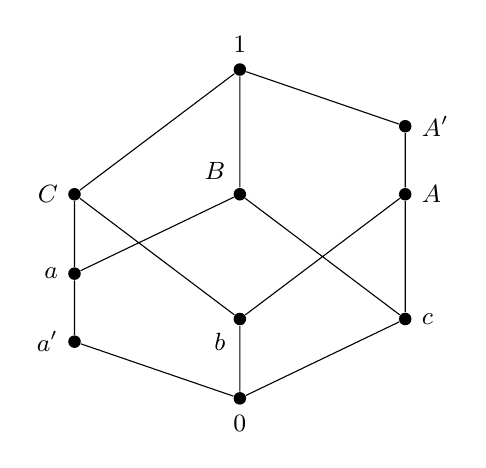
\begin{tikzpicture}[x=1.05cm,y=.72cm,
  dot/.style={circle,fill,inner sep=1.6pt},
  every label/.style={font=\small}]
\node[dot,label=below:$0$] (zero) at (0,0) {};
\node[dot,label=left:$a'$] (ap) at (-2,1) {};
\node[dot,label=left:$a$] (a) at (-2,2.2) {};
\node[dot,label=below left:$b$] (b) at (0,1.4) {};
\node[dot,label=right:$c$] (c) at (2,1.4) {};
\node[dot,label=right:$A$] (A) at (2,3.6) {};
\node[dot,label=above left:$B$] (B) at (0,3.6) {};
\node[dot,label=left:$C$] (C) at (-2,3.6) {};
\node[dot,label=right:$A'$] (Ap) at (2,4.8) {};
\node[dot,label=above:$1$] (one) at (0,5.8) {};
\draw (zero)--(ap)--(a) (zero)--(b) (zero)--(c)
 (a)--(B) (a)--(C) (b)--(A) (b)--(C)
 (c)--(A) (c)--(B) (A)--(Ap)--(one)
 (B)--(one) (C)--(one);
\end{tikzpicture}
\caption{The reconstructed ten-element ortholattice of scan 156-9/113.
Only the marked points are vertices; unmarked edge crossings are not.
The labels refer to the set table in Counterexample~\ref{SA21-A11}.}
\label{fig:ten-element}
\end{figure}
\begin{proof}
The eight sets satisfying the equivalence form an ordered Boolean
cube. Inserting $a'$ between $0,a$ and $A'$ between $A,1$ preserves
existence of binary meets and joins: for an old element $x$, the meet
with $a'$ is $a'$ if $a\leq x$ and $0$ otherwise; its join with
$a'$ is $a'$ if $x=0$, and otherwise the old join $a\vee x$ unless
$x\geq a$, in which case it is $x$. The dual formulas apply to $A'$.
Finally $a'\wedge A'=0$ and $a'\vee A'=1$. These formulas exhaust
the newly introduced pairs. Set complementation interchanges
$a',A'$ and the old complementary pairs, reverses the order, and
has zero meet and unit join on every such pair. Thus it is an
orthocomplementation.
But $a'<a$ and $a\wedge(a')^\perp=a\wedge A'=0$, refuting
orthomodularity. The program checks all 100 pairs and all required
identities. We inspected the original set formula and drawing, not
only the transcription: the second condition in the formula concerns
$i,i'$ both being outside $E$, not $j,i'$. The drawing contains
overwritten construction strokes; the set formula and valid cover
relation above provide the unambiguous mathematical reconstruction.
The lower-right handwritten label has an ambiguous extra stroke;
renaming that vertex $b$ has no mathematical effect.
The transcription also renders the powerset glyph as
$\mathcal P^3(I)$ (line 104). Our ten-element reconstruction uses
$\mathcal P(I)$. If the apparent superscript is instead read literally
as the family of three-element subsets, the displayed predicate selects
only $\{i,i',j\}$, $\{i,i',k\}$, and $\{i',j,k\}$.
They are three incomparable sets, with neither a bottom nor a top;
that reading does not define an ortholattice and cannot have cardinality
ten. The mathematical consequences of these two readings are therefore
distinct, and only the ordinary powerset reading reconstructs the
announced example.
\end{proof}

\subsection{Faithfulness, lieux, and general magasins}

\begin{proposition}[Proved: the faithful case, R1 rechecked]
\label{SA21-A12}
Let $(M,\rho,\perp)$ be a magasin whose interior refinement $\rho$ is
a preorder and whose faithfulness means
\[
 x\perp y\quad\Longleftrightarrow\quad
 \text{there is no }z\text{ with }z\rho x\text{ and }z\rho y.
\]
In the Alexandrov topology of $\rho$-lower sets,
$\Sigma(M)$ is exactly the complete Boolean algebra of regular open
sets. In particular every family of mutually orthogonal supports
satisfies the relative-complement and nonempty-meet conclusions of
the support theorem.
\end{proposition}
\begin{proof}
For $A\subseteq M$ put $O_A=\bigcup_{a\in A}\mathord\downarrow_\rho a$.
Faithfulness says
\[
 N(A)=\operatorname{int}(M\setminus O_A).
\]
Indeed a point belongs to the right side exactly when its principal
lower set meets no principal lower set of a member of $A$.
Since $N(A)$ is open, applying this formula twice gives
$\operatorname{cl}A=\operatorname{int}\overline{O_A}$.
Every such set is regular open; conversely, for a regular open set
$U$, $O_U=U$ and $\operatorname{cl}U=U$. Complement, joins and meets
are consequently the usual regular-open operations. To check the
Boolean assertion without any separation hypothesis on the topology,
if two regular opens have empty intersection, each is contained in
the interior of the complement of the other. Proposition
\ref{SA21-A04}'s lattice argument proves distributivity. In an
Alexandrov topology arbitrary intersections of opens are open; the
intersection of regular opens is regular by monotonicity of
$\operatorname{int}\overline{(-)}$, so the complete meet is their
intersection, as required by the polarity construction.
\end{proof}

\begin{theorem}[Proved: the exact general class under Mag L2]
\label{SA21-A13}
Assume the strong Mag~1--4, divisibility, and the lieu-detection
axiom Mag~L2. Let $L$ be the set of lieux and
$U_X=\{p\in L:p\rho X\}$. In this notation Mag~L2 says
\[
 X\perp Y\iff U_X\perp U_Y.
\]
The maps
\[
 \Sigma(M)\longrightarrow\Sigma(L),\ S\longmapsto S\cap L,
 \qquad
 \Sigma(L)\longrightarrow\Sigma(M),\
 T\longmapsto\widehat T=\{X:U_X\subseteq T\}
\]
are inverse complete ortholattice isomorphisms. Thus the exact class
asked for in A.2 consists of those magasins whose lieu graph satisfies
\eqref{eq:basis-test}. Their Boolean subclass is given exactly by
\eqref{eq:boolean-test} on that graph. Every orthoset occurs as the
lieu graph of a magasin satisfying these hypotheses.
\end{theorem}
\begin{proof}
The axiom forces $U_X\ne\varnothing$, since otherwise it would imply
$X\perp X$. For a lieu $p$, $U_p=\{p\}$.
For any $A\subseteq M$ write $u(A)=\bigcup_{X\in A}U_X$.
The detection formula gives
\[
 N_M(A)=\widehat{N_L(u(A))}.
\]
For any $B\subseteq L$, monotonicity of orthogonality under interior
refinement and the same detection formula give
$N_M(B)\cap L=N_L(B)$ and
$N_M(B)=\widehat{N_L(B)}$.
If $S=N_M(A)$, these identities show
$S=\widehat{S\cap L}$ and $S\cap L$ is closed in $L$.
Conversely, if $T$ is closed in $L$,
$\widehat T=N_M(N_L(T))$ is closed in $M$, and
$\widehat T\cap L=T$. The formulas also show that polars are
preserved, hence all lattice operations are preserved.
To realize an arbitrary orthoset take $M=L=E$, incidence and interior
refinement both identity, and the prescribed orthogonality. The
strong incidence-disjunction condition is vacuous beyond distinct
elements of a singleton principal ideal, and the lifting and
monotonicity axioms are identities. All vertices are lieux and
$U_x=\{x\}$, so divisibility and detection hold. Figures are the
cliques. There is consequently no further hidden restriction on
the class of possible lieu graphs.
\end{proof}

\begin{theorem}[Proved: exact answer to the atom question]
\label{SA21-A14}
In any atelier with the specified orthogonality relation, the nonzero
support $\operatorname{cl}\{x\}$ of a lieu $x$ is an atom if and only if
\begin{equation}\label{eq:atom-test}
 N(x)\subseteq N(y)\quad\Longrightarrow\quad N(x)=N(y)
 \qquad (y\in M).
\end{equation}
Under the hypotheses of Theorem~\ref{SA21-A13}, it suffices to test
$y\in L$. Hence the exact class in A.3 is given by
\eqref{eq:atom-test} for every lieu. The stronger assertion that
$\operatorname{cl}\{x\}=\{x\}$ requires
$N(x)\subseteq N(y)\Rightarrow y=x$ and is different.
\end{theorem}
\begin{proof}
The inclusion of neighbourhoods is equivalent to
$\operatorname{cl}\{y\}\subseteq\operatorname{cl}\{x\}$.
Every nonempty closed set contains the nonempty closure of any one of
its points. Minimality of $\operatorname{cl}\{x\}$ is therefore
equivalent to equality of these singleton closures whenever they
are included. Applying $N$ translates that equality into
\eqref{eq:atom-test}. Under lieu detection, every nonzero closed set
contains a lieu, by the isomorphism and nonemptiness of the $U_X$.
The same proof then restricts the test to lieux. The stronger
singleton statement follows directly from
$y\in\operatorname{cl}\{x\}\iff N(x)\subseteq N(y)$.
\end{proof}

% Insert after Theorem SA21-A14 and its proof.
% AI-produced by GPT-6 Astra (OpenAI), ChatGPT Pro mode, 19 November 2026.
\begin{corollary}[Proved: the exact atom class for interval magasins]
\label{SA21-A14a}
For every poset $L$, the lieux of $M(L)$ are exactly the point symbols
$P_x$. All these lieux have atomic supports if and only if $L$ is an
antichain or $L$ has no isolated points. Thus every lieu has an atomic
support for every nonempty connected poset, including the singleton.
For $L=\varnothing$ the assertion is vacuous.
\end{corollary}
\begin{proof}
We use the manuscript's full-refinement definition of a lieu:
minimality for $\ll$, not merely for interior refinement $\rho$
(156-8, scan~15, \path{J156-8-02_transcription.tex:277}).
In the primed formulation it is minimality for both incidence and
$\rho$ (\path{J156-8-04_transcription.tex:282,296}).
Only $P_x$ refines $P_x$, since a factorization
$U\rho Z\le P_x$ forces $Z=P_x$ and then $U=P_x$.
Every interval $I_{ab}$ has the distinct incidence predecessor
$P_a$, which also refines it. Thus the lieux are exactly the points,
even when $a\lessdot b$ makes $I_{ab}$ minimal for $\rho$ alone.
In particular we make no unsupported divisibility claim for intervals
having no point strictly between their endpoints.

Theorem~\ref{SA21-A06} proves that every nonisolated $x$ has
$\operatorname{cl}\{P_x\}=\{P_x\}$, a nonzero atom.
For an isolated $x$, the symbol $P_x$ has no neighbour, so
$\operatorname{cl}\{P_x\}=M(L)$. If $L$ has a comparison $a<b$,
the singleton support of $P_a$ is a proper nonzero closed set,
and this top support is not an atom. If $L$ is a nonempty antichain,
there are no interval symbols and no disjunction edges; its support
lattice has just zero and one, so every lieu has that single nonzero
atom as support. These alternatives prove both directions of the
criterion. A connected comparability graph with more than one vertex
has no isolated point, and the singleton case is an antichain.
The empty case follows from the universal quantifier over no lieux.
\end{proof}


\begin{counterexample}[Refuted inference; R2 and L3 precisely qualified]
\label{SA21-A15}
Two lieux with no edge have the two-element Boolean support lattice;
their supports are the same atom. Thus nondisjoint distinct lieux do
not, by themselves, measure failure of distributivity. Under Mag~L2
and divisibility, the following are equivalent: faithfulness;
Booleanity with lieux represented by distinct atoms; and
$p\perp q$ for every pair of distinct lieux. In the additional
point-separating case $\operatorname{cl}\{p\}=\{p\}$ for all lieux,
Booleanity alone is equivalent to pairwise disjointness of distinct
lieux. Without point separation the exact replacement is
Theorem~\ref{SA21-A04}.
For interval magasins the exact replacement is the nonisolated-core
criterion of Theorem~\ref{SA21-A06}. In particular, for a connected
poset $L$, Booleanity of $\Sigma_{M(L)}$ is equivalent to totality
of $L$, hence to disjointness of distinct lieux. Thus this precise
connected interpretation of the qualitative claim in L3 is true.
The unqualified claim fails even in a divisible interval magasin
with genuine interval strata: take $L=\mathbb Q\amalg\{c\}$,
with $c$ incomparable to every rational.
\end{counterexample}
\begin{proof}
The two-vertex graph has $N(\varnothing)=L$ and $N(A)=\varnothing$
for every nonempty $A$, proving the first claim and also showing why
the atom question is weaker than separation.
Faithfulness on distinct lieux forces orthogonality, since they have
no common interior lower bound. Conversely if distinct lieux are
orthogonal, detection says $X\not\perp Y$ precisely when
$U_X\cap U_Y\ne\varnothing$. This is equivalent to a common
interior refinement: a common lieu is one, and any common refinement
contains a lieu. Thus the magasin is faithful. Its support lattice
is $\mathscr P(L)$ under Theorem~\ref{SA21-A13}, with distinct
singleton atoms. Conversely distinct atoms of a Boolean algebra are
orthogonal, so the corresponding lieux are orthogonal. The same
argument proves the last assertion when singleton separation is
assumed. The four-lieu graph consisting of two disjoint edges gives
$MO_2$: its supports are zero, the four singletons, and one; it is
orthomodular but not distributive. This is also checked in the code.

For the connected assertion, a connected comparability graph with
at least two vertices has no isolated vertex, so its nonisolated
core is all of $L$. The empty and singleton cases cause no exception.
Apply Theorem~\ref{SA21-A06}; the lieux of an interval magasin are
its point symbols, whose disjunction is strict comparability.

For the final example the nonisolated core is the chain $\mathbb Q$,
so Theorem~\ref{SA21-A06} proves Booleanity. Every interval $I_{ab}$
has nonempty open-lieu set $\{P_q:a<q<b\}$, by density of
$\mathbb Q$, and point symbols have singleton open-lieu sets.
Two rational interval interiors are disjoint precisely when their
endpoints are positionally ordered; a rational point is orthogonal to an
interval precisely when it is outside that interval's open interior.
Together with the singleton tests this proves Mag~L2 and divisibility.
The extra lieu $P_c$ is orthogonal to no symbol, and each other open
lieu set is nonempty, so the same detection test also holds for every
pair involving it. Nevertheless $P_c\not\perp P_q$ for all rational
$q$. Its singleton support is the top, since $N(P_c)=\varnothing$.
This gives the asserted failure inside the interval construction
itself, and explains why point separation is the missing hypothesis.
\end{proof}

\subsection{The exact support theorem and the distinction from orthomodularity}

\begin{theorem}[Proved: complete characterization of A.4]
\label{SA21-A16}
Fix an orthoset $E$ and a family $(U_i)_{i\in I}$ of nonempty mutually
orthogonal subsets. Put $e_i=\operatorname{cl}U_i$,
$S_A=\operatorname{cl}(\bigcup_{i\in A}U_i)$ for $A\subseteq I$,
and $S=S_I$. The map $A\mapsto S_A$ is always an injective order map
preserving arbitrary joins. The following explicit condition is
necessary and sufficient for the remaining lattice conclusions
(a)--(c) of the Théorème of 156-7, scan 94:
\begin{equation}\label{eq:figure-test}
\begin{gathered}
 z\in S,\quad w\in E,\quad
 (\forall i\in I)\ [z\perp U_i\ \text{or}\ w\perp U_i]
 \quad\Longrightarrow\quad z\perp w.
\end{gathered}
\end{equation}
More precisely this is equivalent to all identities
\[
 S_A\cap N\Bigl(\bigcup_{i\in B}U_i\Bigr)=S_{A\setminus B}
 \qquad(B\subseteq A\subseteq I),
\]
and it implies preservation of arbitrary nonempty meets. Empty meets
are preserved into the interval $[0,S]$; they are preserved into the
whole lattice only when $S=1$.
For the atelier specialization take $I=\widetilde F$ for an admitted
figure $F$, and $E=M$ with the \emph{old
whole-figure disjunction} $\parallel$, and write $N_\parallel$
for its polar. Here $U_X$ are the actual open-stratum subsets used
to define $S_A$, or subsets with the same polars as justified below.
For every incidence-closed subfigure $G\leq F$, clause (d) has the
additional exact criterion
\begin{equation}\label{eq:incidence-coverage}
 N_\parallel(\widetilde G)
 =N_\parallel\Bigl(\bigcup_{X\in\widetilde G}U_X\Bigr).
\end{equation}
Here $\operatorname{Supp}(G)=N_\parallel^2(\widetilde G)$.
Under the older hypotheses of scan 94, nonemptiness, mutual
orthogonality and \eqref{eq:incidence-coverage} are automatic;
the exact class asked for in A.4 is then given by
\eqref{eq:figure-test} for every admitted figure. If those hypotheses
are dropped, include all three of these requirements explicitly.
Injectivity forces nonemptiness, and the relative-complement formula
for two different indices forces orthogonality. This formulation
applies to infinite figures and infinite families.
\end{theorem}
\begin{proof}
Joins are preserved by idempotence of closure. If $i\in A\setminus B$,
then $0\ne e_i\leq S_A$ and $e_i\perp S_B$, so $S_A\not\leq S_B$.
This proves order reflection and injectivity.
Assume \eqref{eq:figure-test}. If
$z\in S\cap N(\bigcup_{i\in A}U_i)$, and
$w\in N(\bigcup_{i\notin A}U_i)$, its hypothesis holds for every
$i$, so $z\perp w$. Thus $z\in S_{I\setminus A}$. The reverse
inclusion follows from mutual orthogonality and monotonicity.
Conversely, assume this relative-complement identity for every $A$.
Given the hypothesis of \eqref{eq:figure-test}, choose
$A=\{i:z\perp U_i\}$. Then $w$ is orthogonal to all $U_i$ outside
$A$, while $z\in S\cap N(\bigcup_{i\in A}U_i)=S_{I\setminus A}$;
hence $z\perp w$.
It remains to prove that the single-top identity gives all the stated
operations. Write $c_S(T)=S\cap T^\perp$. On the image of our map it
is the involution $S_A\mapsto S_{I\setminus A}$. Therefore, for a
nonempty family $(A_j)$,
\[
\begin{split}
 \bigcap_j S_{A_j}
 &=S\cap\bigcap_j S_{I\setminus A_j}^{\perp}
 =S\cap\Bigl(\bigvee_j S_{I\setminus A_j}\Bigr)^\perp\\
 &=S\cap S_{\bigcup_j(I\setminus A_j)}^\perp
 =S_{\bigcap_j A_j}.
\end{split}
\]
Intersecting $S_A$ with $S\cap S_B^\perp=S_{I\setminus B}$ gives
the full relative-complement formula. The case of the empty family
has meet $S$ in $[0,S]$ and meet $1$ in the ambient lattice, proving
the necessary edge-case qualification.

We verify clause (d) and the comparison with the manuscript's open
sets, instead of silently substituting lieux for strata. Write
$\ell(X)=\{p:p\text{ is a lieu and }p\ll X\}$ and
$V_X=\ell(X)\setminus\ell(\partial X)$. At scan 90 the open
representative is
\[
 X^\circ=\{Y\in M:Y\ll X,\ Y\parallel\partial X\}.
\]
The old L3 and L2 imply $V_X\subseteq X^\circ$. If
$Y\in X^\circ$, then $\ell(Y)\subseteq\ell(X)$ and no lieu
of $Y$ belongs to $\ell(\partial X)$, since such a lieu would
be disjoint from itself. Thus $\ell(Y)\subseteq V_X$.
Testing disjunction using old L2 now gives
$N_\parallel(X^\circ)=N_\parallel(V_X)$, so both choices give
exactly the support map stated at scans 93--94.
The earlier scan-87 definition is
$\operatorname{Supp}(X)\cap N_\parallel(\partial X)$.
Old absorption At supp~1 puts its members among refinements of $X$;
the reverse inclusion for the scan-90 representative follows from
hereditary disjointness, which gives
$Y\ll X\Rightarrow Y\in\operatorname{Supp}(X)$.
Hence those two open-set definitions agree under the hypotheses
being used here.

Finally, carriers give
$\ell(G)=\bigcup_{X\in\widetilde G}V_X$. For any $Z\in M$,
old L2 says that $Z\parallel G$ exactly when every lieu of $Z$
is disjoint from every lieu of $G$. Substituting this union and
applying L2 to $Z$ and each singleton lieu gives exactly
\eqref{eq:incidence-coverage}, for $U_X=V_X$ and therefore also
for $U_X=X^\circ$. Applying the polar once more proves
$S_{\widetilde G}=\operatorname{Supp}(G)$, clause (d).
Without the older hypotheses, equality of these two closed sets
is equivalent to equality of their polars, so the displayed
additional criterion is both necessary and sufficient. Empty $G$
is included, since both unions are empty.
\end{proof}

\begin{theorem}[Proved: the exact relation with orthomodularity]
\label{SA21-A17}
In a complete orthomodular lattice, every mutually orthogonal family
of nonzero elements satisfies the lattice clauses (a)--(c) of
Theorem~\ref{SA21-A16}. Conversely, if the relative-complement formula
holds for every two-element orthogonal family of nonzero lattice
elements, the lattice is orthomodular. Thus 156-9, scan 117, applied
to the universal spatial figures of a spatios, is equivalent to
orthomodularity. The axiom for the actual figures of a given magasin
is weaker, even under Mag~1--4, divisibility and Mag~L2.
\end{theorem}
\begin{proof}
For orthogonal $u,v$ in an orthomodular lattice the dual
orthomodular law gives
$(u\vee v)\wedge u^\perp=v$. For any subset $A$ of an orthogonal
family, let $u=\bigvee_{i\in A}e_i$ and
$v=\bigvee_{i\notin A}e_i$. Completeness and order reversal of
orthocomplement give $u\perp v$; the displayed identity gives the
relative-complement formula for $S_I=u\vee v$. This argument treats
infinite families directly. Theorem~\ref{SA21-A16} supplies the other
lattice conclusions. It is also a direct form of the commuting-element
calculus usually derived from the Foulis--Holland theorem.
Conversely, for $a\leq b$ apply the assumed identity to
$u=b^\perp$ and $v=a$; zero terms may be omitted. It yields
$(b^\perp\vee a)\wedge b=a$. Taking orthocomplements gives
$a^\perp=(b\wedge a^\perp)\vee b^\perp$, the orthomodular law
for $b^\perp\leq a^\perp$. Thus it holds for every comparable pair.
For strictness, use the graph of Counterexample~\ref{SA21-A07} with
identity incidence and identity interior refinement, so all eight
vertices are lieux. Theorem~\ref{SA21-A13} verifies every magasin
hypothesis. Theorem~\ref{SA21-A08} proves Axiome supp~1 for every
figure, whereas its twenty-element support lattice is not
orthomodular. Actual figures do not realize every orthogonal pair of
abstract supports, which is exactly the missing quantifier.
\end{proof}

\begin{counterexample}[Refuted: the disjunctive-magma support axiom]
\label{SA21-A18}
Take four lieux $a',a,b,b'$ with identity incidence and interior
refinement and only the edges $a'a,ab,bb'$.
Then every strong Mag axiom, divisibility and Mag~L2 hold, but
Axiome supp~1 fails for $F=\{a,b\}$:
\[
 \operatorname{cl}F=E,\qquad
 \operatorname{cl}F\cap N(a)=\{a',b\}\ne\{b\}
     =\operatorname{cl}\{b\}.
\]
Its support lattice is $O_6$. If ``disjunctive'' is given the stronger
spatial interpretation in which interior refinement is reconstructed
from supports, use instead the five-cycle with identity incidence
and interior refinement: its singleton supports are singletons, so
that reconstruction is identity, and the same axiom fails. Thus
both readings of the request after the marginal ``Oui!'' of 156-8,
scan 89, have an explicit counterexample.
\end{counterexample}
\begin{proof}
The identity-incidence construction was verified in
Theorem~\ref{SA21-A13}. The six closed sets are
$\varnothing,\{a\},\{b\},\{a,b'\},\{a',b\},E$.
The neighbourhood calculation proves the displayed failure, and
their inclusion order is the six-element ortholattice hexagon.
For the five-cycle the calculation is in
Counterexample~\ref{SA21-A19}. The attached code checks every subset
and every finite axiom for both examples.
\end{proof}

\begin{counterexample}[Refuted under the older hypotheses as well]
\label{SA21-A19}
The five-cycle with identity incidence and refinement is an atelier
satisfying the older At~1--7, At~L1--L3, CL(spac), At~D, At~supp and
the old absorption axiom At~supp~1 of 156-7, scan 87. Nevertheless
the relative-complement conclusion of scan 94 fails, so the theorem
as a whole is false under its stated hypotheses.
\end{counterexample}
\begin{proof}
Every vertex is a lieu, every point closure is a singleton, and the
figures are the empty set, the five vertices and the five edges.
Compatibility is clique-union, figure incidence and refinement are
inclusion. The elementary figures are singletons. This explicitly
gives At~1--7, the lifting and decomposition requirements, and
At~L1--L3. Local compatibility and disjunction are exactly their
pointwise tests, so CL(spac) and At~D hold. If $G\ll X$ with $X$
elementary, either $G=X$, when the support-separation premise is
false, or $G=\varnothing$, when $X$ itself is the required witness;
this verifies old At~supp. Finally $X^\circ=\operatorname{cl}\{X\}
=\{X\}$ proves the old absorption axiom.
Number the cycle modulo five and take $F=\{0,1\}$. Then
$\operatorname{cl}F=E$ and
$E\cap N(0)=\{1,4\}\ne\{1\}=\operatorname{cl}\{1\}$.
For meet preservation it is essential that the indexing members
belong to one figure: in this edge figure,
$S_{\{0\}}\cap S_{\{1\}}=0$ does hold, so this particular
counterexample establishes the complement failure alone. No claim
about meets is inferred merely from this calculation; the original
eight-stratum example is treated separately below.
\end{proof}

\subsection{A faithful support function that is not fully faithful}

\begin{counterexample}[Proved: answer to A.5]\label{SA21-A20}
Let $M=\{a,b\}$, with identity incidence, interior refinement
$a\rho b$ in addition to identities, and no internal disjunction.
The figures are $\varnothing,\{a\},\{b\}$.
Let $P=\{p,q\}$ and define the external support function
\[
 |a|=\{p\},\qquad |b|=\{p,q\}.
\]
It is faithful and normalized, but not fully faithful in the exact
sense of 156-8, scan 86.
\end{counterexample}
\begin{proof}
Interior refinement is a partial order. Incidence lifting is trivial;
orthogonality monotonicity and the strong incidence axiom are
vacuous. Both principal interior lower sets contain $a$, so the
magasin itself is faithful. Since incidence is identity, external
open and full supports coincide. They are nonempty, monotone under
interior refinement, and their intersections are always nonempty.
Thus they detect exactly the prescribed empty disjunction relation.
They cover $P$ and distinguish its two points, satisfying the usual
normalization and separation conventions as well.
Full faithfulness requires, for a figure $F$,
\[
 \bigcup_{Z\perp F}|Z|^\circ=P\setminus|F|.
\]
For $F=\{a\}$ the left side is empty, while the right side is
$\{q\}$. Hence full faithfulness fails. This property is not
equivalent to reflecting refinement, and a constant singleton
support function would not provide the required counterexample.
\end{proof}

\subsection{Spatios, disjoncteurs, and their actual morphisms}

\begin{theorem}[Proved: the object dictionary and its zero convention]
\label{SA21-A21}
A spatios satisfying Spat~1--3 of 156-9, scans 51--53 and 78--80,
is exactly a complete ortholattice. For a complete ortholattice $K$,
put $E_K=K\setminus\{0\}$ and $x\perp y\iff x\leq y^\perp$.
Then
\[
 K\longrightarrow\Sigma(E_K),\quad
 s\longmapsto\{x\ne0:x\leq s\}
\]
is a complete ortholattice isomorphism. If zero is retained, the
relation is not irreflexive; the manuscript allows a self-orthogonal
point only when it is orthogonal to every point. Removing this
radical is the exact comparison with ordinary orthosets.
\end{theorem}
\begin{proof}
Spat~1 is completeness of the order, Spat~2 is an order-reversing
involution, and Spat~3 is the zero-meet complement identity; the
unit-join identity follows by the involution. These are precisely
the stated ortholattice axioms. For $A\subseteq E_K$, its polar is
the nonzero principal ideal below $(\bigvee A)^\perp$, and its
double polar is the nonzero principal ideal below $\bigvee A$.
All such ideals occur, and inclusion and complement give the claimed
isomorphism. If a symmetric relation has radical $R$ consisting of
its self-orthogonal points and each such point is universally
orthogonal, every closed set contains $R$. Removing $R$ and adding
it back are inverse isomorphisms of the resulting support lattices.
The empty orthoset represents the one-element spatios.
\end{proof}

\begin{theorem}[Proved: the correspondence category; L7 corrected]
\label{SA21-A22}
Let $E,F$ be orthosets. A saturated correspondence of the final
156-9 construction is a map $\alpha:E\to\Sigma(F)$ such that
\begin{equation}\label{eq:bond}
 x\in\operatorname{cl}_E A\quad\Longrightarrow\quad
 \alpha(x)\subseteq\bigvee_{a\in A}\alpha(a)
 \qquad(A\subseteq E).
\end{equation}
It corresponds bijectively to a complete join-preserving map
$f:\Sigma(E)\to\Sigma(F)$ by
\[
 f(S)=\bigvee_{x\in S}\alpha(x),\qquad
 \alpha(x)=f(\operatorname{cl}_E\{x\}).
\]
Composition is
$(\beta\alpha)(x)=\bigvee_{y\in\alpha(x)}\beta(y)$ and the identity
is $x\mapsto\operatorname{cl}\{x\}$.
If $g$ is the order right adjoint of $f$, the transposed
correspondence induces
$f^\dagger=C_EgC_F$, characterized by
\[
 f(S)\perp T\quad\Longleftrightarrow\quad S\perp f^\dagger(T).
\]
Consequently orthosets with these correspondences are equivalent
as a category to complete ortholattices with all complete join maps.
They are not the category of orthosets with ordinary functions
preserving orthogonality. L7 is false with that unqualified morphism
claim and true only with this explicit object and arrow dictionary.
\end{theorem}
\begin{proof}
If $f$ preserves all joins, including the empty join, the displayed
definition of $\alpha$ gives \eqref{eq:bond}, because
$\operatorname{cl}A=\bigvee_{a\in A}\operatorname{cl}\{a\}$.
Conversely, \eqref{eq:bond} implies
$\bigvee_{x\in\operatorname{cl}A}\alpha(x)=
\bigvee_{a\in A}\alpha(a)$, so the stated $f$ preserves joins.
Putting $A=\{x\}$ and using $x\in\operatorname{cl}\{x\}$ proves
that the two assignments are inverse. The composition and identity
formulas follow by substituting these expressions and associating
joins.
The right adjoint exists for any complete join map and is
$g(T)=\bigvee\{S:f(S)\leq T\}$. Therefore
\[
 f(S)\leq C_FT\iff S\leq g(C_FT)
       \iff S\perp C_Eg(C_FT).
\]
Since $g$ preserves meets, $C_EgC_F$ preserves joins. The displayed
adjunction characterizes it uniquely, proves involutivity of the
dagger and reverses composition. Equivalently,
\eqref{eq:bond} says that for every $y\in F$ the column
$\{x:\alpha(x)\perp y\}$ is closed: either implication follows
by applying the respective closure condition to that column.
This is the two-sided saturation of the relation in 156-9,
scans 95--100. The object functor is essentially surjective by
Theorem~\ref{SA21-A21}, and the arrow bijection is full and faithful,
which proves the claimed categorical equivalence.
For the failure of the ordinary-function interpretation, take
classical orthosets, with $x\perp y\iff x\ne y$.
Their support lattices are powersets and every relation gives a
complete join map. A relation sending one point to two points is
not a function. A relation sending two distinct points to the same
point is a function but does not preserve orthogonality. Both are
saturated correspondences. The finite certificate includes these
two examples. Earlier uses of the word ``morphism'' in the notes
have different extra requirements and are not silently identified
with this final correspondence category.
\end{proof}

\begin{theorem}[Proved: the typed spatial reconstruction]
\label{SA21-A23}
Let $(E,\preceq,\perp)$ have a partial incidence order and an
orthoset relation. For each $x$ label its principal incidence ideal
by $y\mapsto\operatorname{cl}\{y\}$, transporting the incidence
order. Assume that these labels form an elementary ordered spatial
figure: the labels are nonzero, distinct, and pairwise orthogonal.
Assume also that the resulting ordered deployment $D_x$ determines
$x$ injectively. There is then a unique spatial interior refinement
making these data a strong magasin. It is given by the existence
of an order-preserving carrier
\[
 h:D_x\longrightarrow D_y,\qquad S\subseteq h(S),
 \qquad h(\operatorname{cl}\{x\})=\operatorname{cl}\{y\}.
\]
This is the fully typed interpretation of At~spat~1--3 in 156-9,
scan 50, using the spatial target explicitly defined on scan 48.
If that target is read merely as disjoint subsets of $E$, the
assertion is false and strong At~4 must be added.
\end{theorem}
\begin{proof}
The carrier, when it exists, is unique: a nonzero closed set cannot
lie below two different orthogonal labels in $D_y$. Identities and
composition prove reflexivity and transitivity. If carriers exist
in both directions, their composites send each label $S$ to a label
$U$ of the same deployment with $S\subseteq U$. Distinct labels
there are orthogonal, so $S=U$; the intermediate inclusion is also
equality. The deployments and their transported orders coincide,
and injectivity gives $x=y$. Thus the relation is a partial order.
If $z\preceq x$, restricting a carrier to $D_z$ lands in the
principal ideal below its value on the top label of $D_z$; that ideal
is the deployment of the corresponding stratum of $y$. This proves
incidence lifting and uniqueness. Allowing a carrier without the
top-preserving condition gives exactly its composite with incidence:
factor through the principal ideal below the top image. Internal
orthogonality is monotone because the top labels are included, and
two distinct strata under one incidence top are orthogonal by the
typed deployment hypothesis. These are strong Mag~1--4. The
carrier description is precisely the sufficient ``Raff'' condition
defining spatiality on scans 46--47, and it also proves uniqueness.
For the weaker interpretation use the five-cycle orthoset with
incidence $0,2\prec1$ and all other incidences identities. Its
singleton closures are singletons. All deployments are distinct
ordered families of disjoint nonempty subsets, and comparable
distinct strata are orthogonal. But the two strata $0,2$ below $1$
are not orthogonal, violating strong At~4. This finite example is
checked by the program. Scan 47's margin and scan 49 explicitly
retain At~4, consistent with the corrected typed formulation.
\end{proof}

\begin{counterexample}[Proved: R5's simultaneous failures rechecked]
\label{SA21-A24}
The supplied eight-stratum example satisfies its stated older
hypotheses, and both nonempty-meet preservation and relative
complementation fail in one figure. Its complete data are
\[
 M=\{a,b,X,p,e,w,h,g\},\qquad a,b\lhd X,\quad p\rho X,
\]
with no other nonidentity generating incidences or interior
refinements. The lieu graph on $\{a,b,p,e,w,h,g\}$ has edges
\[
 ab,ap,bp,ae,bw,pw,eh,hg,gw.
\]
Internal disjunction adds $Xa,Xb,Xw$. Old full figure-disjointness
has the displayed lieu edges and no edge at $X$.
\end{counterexample}
\begin{proof}
The only nontrivial principal incidence figure is $\{a,b,X\}$;
its three strata are internally orthogonal. Interior refinement
has the sole nonidentity relation $p\rho X$, and the neighbours
of $X$ are exactly those of $p$, proving monotonicity. Incidence
lifting for $p\rho X$ is immediate, since $p$ has no proper face.
Every stratum has a lieu in its open shadow. Detection by lieu
shadows holds by the specified edges, and compatibility and full
disjunction are the corresponding pairwise tests on the principal
figures. This proves strong Mag~1--4 and the older L1--L3 and
CL(spac), which imply the older relative C and D conditions by the
carrier construction. For completeness the program enumerates all
figures, all their restrictions, and every instance of the older
support-separation axiom; all pass.
The full-disjunction singleton closures of the seven lieux are
singletons. The full support of $X$ is $M$, and
$X^\circ=M\cap N(\{a,b\})=\{p\}$; thus old absorption holds for
every multistrate. In the figure $F=\{a,b,X\}$ the open strata are
$\{a\},\{b\},\{p\}$. Direct intersections of neighbourhoods give
\[
\begin{aligned}
 S_F\cap S_a^\perp&=\{b,p,e\},& S_{\{b,X\}}&=\{b,p\},\\
 S_{\{a,X\}}\cap S_{\{a,b\}}&=\{a,w\},&S_{\{a\}}&=\{a\}.
\end{aligned}
\]
Both inequalities are strict. The certificate lists all eighteen
closed sets for the full-disjunction graph, the open parts of all
eight multistrates, all axiom flags, and the displayed witnesses.
This rechecks SA21-K7b-15 and SA21-R7b-21 rather than inferring them
from the smaller five-cycle example.
\end{proof}

\begin{proposition}[Proved: the cograph sufficient condition is strict]
\label{SA21-A25}
Every finite cograph has an orthomodular support lattice. The converse
fails even for a five-element comparability poset with a Boolean
support lattice.
\end{proposition}
\begin{proof}
We use the recursive definition of cographs: start with one vertex
and close under disjoint union and graph join. For graph join, the
polarity acts coordinatewise on the vertex parts; the support
ortholattice is the product of their support ortholattices. For a
disjoint union of nonempty graphs, every proper nonzero closed set
lies in a single component, and is a proper nonzero closed set of
that component. Its orthocomplement is the corresponding component
complement. Thus the support lattice is their horizontal sum,
identifying all zeros and all units; a two-element factor contributes
no proper element. Both products and horizontal sums of
orthomodular lattices are orthomodular: a comparable proper pair in
a horizontal sum lies in the same factor, and the pairs involving
zero or one satisfy the law directly. Induction proves the claim.
For strictness, let the five points represent the nonempty subsets
$\{1\},\{2\},\{3\},\{1,2\},\{2,3\}$, orthogonal when disjoint.
The three singletons separate all subsets of $\{1,2,3\}$, so the
closed sets are exactly the intersections of these five points with
the principal ideals of $\mathscr P(\{1,2,3\})$; the lattice is
Boolean with eight elements. Write the singleton points as $a,b,c$
and the other two as $x,y$. The graph has edges $ab,ac,bc,cx,ay$ and
contains the induced path $x-c-a-y$. It is a comparability graph:
orient its edges by $a<b<c$, $x<c$, $a<y$. These comparisons are
transitive and introduce no extra edges. The explicit graph and its
eight closed sets are checked in the certificate. This verifies the
substance of R14's strictness without relying on its earlier
enumeration counts.
\end{proof}

\IfFileExists{parts/supports/supports_transfer.tex}{% AI-produced by GPT-6 Astra (OpenAI), ChatGPT Pro mode, 19 November 2026.
% Additional Part A proof. No priority claim. Uses the master's theorem counter.

\subsection{The split-poset comparison and the finite classification}
\label{sec:split-poset-comparison}

For a poset $P$, write
\[
 Q^+(P)=\{[u<v]:u,v\in P,\ u<v\},
 \qquad [u<v]\perp[r<s]\iff v\le r\ \text{or}\ s\le u.
\]
This is the orthogonality space of proper quotients in
\citet[\S4, p.~6]{Jenca2022}. Its order by interval inclusion is a
different relation. We write $\mathcal C(O)$ for the complete
ortholattice of double-polar closed subsets of an orthogonality space
$O$; complements and polars below are always taken in the indicated
ambient space.

\begin{theorem}[Proved: the comparison for every ordered set]
\label{SA21-A26}
For an arbitrary poset $L$, let $S(L)=L\times\{-,+\}$ with
$x^-<x^+$ and $x^\epsilon<y^\delta$ whenever $x<y$ in $L$.
The maps
\[
 P_x\longmapsto[x^-<x^+],\qquad
 I_{a,b}\longmapsto[a^+<b^-]\quad(a<b)
\]
embed the disjoncteur of $M(L)$ as an induced subspace $U$ of
$Q^+(S(L))$. They induce an isomorphism of complete ortholattices
\[
 \Sigma_{M(L)}\cong\mathcal C\bigl(Q^+(S(L))\bigr).
\]
The isomorphism and its inverse are given explicitly by trace and by
the finite-piece extension described in the proof. No finiteness,
boundedness, connectedness or existence of meets and joins is assumed.
\end{theorem}
\begin{proof}
The three types of orthogonality in $M(L)$ are
\begin{align*}
 P_x\perp P_y&\iff x<y\ \text{or}\ y<x,\\
 P_x\perp I_{a,b}&\iff x\le a\ \text{or}\ b\le x,\\
 I_{a,b}\perp I_{c,d}&\iff b\le c\ \text{or}\ d\le a.
\end{align*}
Substitution in the displayed quotient relation gives exactly these
conditions, including the endpoint equalities. Thus the embedding is
an induced orthogonality embedding.

Every $q=[a^\epsilon<b^\delta]$ with $a<b$ is a concatenation of
at most three members of $U$: include $[a^-<a^+]$ if $\epsilon=-$,
always include $[a^+<b^-]$, and include $[b^-<b^+]$ if $\delta=+$.
Call this finite set $D(q)$. If both endpoints have the same base
element, then $q=[a^-<a^+]\in U$ and $D(q)=\{q\}$.
In every case the pieces have successive common endpoints and together
run from the first endpoint of $q$ to its last endpoint. Consequently,
for every $r\in Q^+(S(L))$,
\begin{equation}
 \label{eq:MT-pieces}
 q\perp r\quad\Longleftrightarrow\quad
 d\perp r\text{ for every }d\in D(q).
\end{equation}
The forward implication follows from interval containment. For the
reverse implication, write the pieces as
$[c_0<c_1],\ldots,[c_{k-1}<c_k]$ and $r=[v<w]$.
For each piece either $c_i\le v$ or $w\le c_{i-1}$.
If both alternatives occur at consecutive positions, they imply
$w\le c_i\le v$, contradicting $v<w$. Thus all pieces lie on the
same side of $r$, giving $c_k\le v$ or $w\le c_0$, as required.

For $B\subseteq U$, set
\[
 E(B)=\{q\in Q^+(S(L)):D(q)\subseteq B\}.
\]
We identify $U$ with $M(L)$ via the embedding. Equation
\eqref{eq:MT-pieces} gives
$B^{\perp_{Q}}=E(B^{\perp_U})$.
More generally,
\[
 E(B)^{\perp_Q}=E(B^{\perp_U}).
\]
Indeed testing orthogonality to $E(B)$ includes testing every $b\in B$
because $D(b)=\{b\}$; conversely the pieces of every element of
$E(B)$ belong to $B$, so the same test suffices. Hence
$E(B)^{\perp_Q\perp_Q}=E(B^{\perp_U\perp_U})$.
In particular $E$ takes closed sets to closed sets, commutes with
complement, and its trace on $U$ is $B$.

Conversely let $A\subseteq Q^+(S(L))$ be closed. If $q\in A$, then
every piece of $q$ is orthogonal to $A^{\perp_Q}$ by
\eqref{eq:MT-pieces}, and hence belongs to $A$. Conversely if every
piece lies in $A$, that same equation gives $q\in A$. Therefore
$A=E(A\cap U)$. The preceding polar formula then shows that $A\cap U$
is closed in $U$. Thus trace and $E$ are mutually inverse order
isomorphisms preserving orthocomplement; consequently they preserve
all meets and joins. This proves the complete-ortholattice comparison,
including the empty case.
\end{proof}

We call $P$ a \emph{conditional lattice} when every pair having a common
upper bound has a least upper bound and every pair having a common
lower bound has a greatest lower bound. We do not require a global
least or greatest element.

\begin{lemma}[Proved: finite conditional lattices suffice for quotient spaces]
\label{SA21-A27a}
If $P$ is a finite conditional lattice, then $\mathcal C(Q^+(P))$
is orthomodular.
\end{lemma}
\begin{proof}
Adjoin two new strict bounds $\widehat0,\widehat1$ to form
$\widehat P$. This is a finite lattice: joins or meets already present
in $P$ are retained, and a pair with no upper, respectively lower,
bound in $P$ has join $\widehat1$, respectively meet $\widehat0$.
Let $X$ be closed in $Q^+(P)$ and put
$\widehat X=X^{\perp\perp}$ in $Q^+(\widehat P)$.
Then
\begin{equation}
 \label{eq:MT-trace}
 \widehat X\cap Q^+(P)=X.
\end{equation}
To verify the possibly delicate inclusion, a point of the left side
is orthogonal to every element of $X^{\perp}$ in the larger space,
hence to every element of its trace, which is exactly the polar in
$Q^+(P)$. Since $X$ is closed in the smaller space, the point belongs
to $X$. The reverse inclusion is extensivity of closure.

By \citet[Theorem~4.10(a)$\Rightarrow$(b), p.~10]{Jenca2022}, the
closed set $\widehat X$ is of chain type: it is a finite union of
full quotient intervals
\[
 [a_1<b_1]^{\downarrow}\ \cup\cdots\cup\
 [a_k<b_k]^{\downarrow},
 \qquad a_1<b_1<a_2<b_2<\cdots<a_k<b_k
\]
in $\widehat P$. We have retained both finiteness and boundedness
when invoking this theorem. Taking traces gives an orthogonal union
$X=X_1\cup\cdots\cup X_k$. A nonempty trace block is one of the
following: all quotients in $[a,b]\subseteq P$; all quotients whose
upper endpoint is at most $b$; all quotients whose lower endpoint is
at least $a$; or all of $Q^+(P)$. The last three cases arise only from
a new endpoint $\widehat0$ or $\widehat1$.

Let $B$ be any maximal pairwise orthogonal subset of $X$. Since the
blocks are mutually orthogonal, $B_i=B\cap X_i$ is maximal in $X_i$.
We show directly that $B_i^{\perp}=X_i^{\perp}$, with both polars
taken in $Q^+(P)$; we do not assume that an individual trace block
is itself closed. The case $X_i=\varnothing$ is immediate. In a
nonempty block, order the finite quotient family $B_i$ from left to
right. Its intervals have successive endpoints
\[
 [c_0<c_1],\ [c_1<c_2],\ \ldots,\ [c_{r-1}<c_r].
\]
There can be no gap between consecutive intervals, since the quotient
across that gap would lie in $X_i$ and enlarge $B_i$.
For a bounded block $[a,b]$, maximality also forces $c_0=a,c_r=b$.
By the concatenation argument in \eqref{eq:MT-pieces}, a quotient is
orthogonal to $B_i$ precisely when it lies below $a$ or above $b$;
that is exactly orthogonality to the entire block.

For a lower-ray block, maximality forces $c_r=b$ and makes $c_0$
minimal in all of $P$: any $p<c_0$ would still satisfy $p<b$ and
would supply an additional quotient in this block. Thus no proper
quotient of $P$ can lie below $c_0$. Its polar consists exactly of
the quotients above $b$, the polar of the whole block. The upper-ray
case is dual. For the whole space, a maximal orthogonal family has
no common orthogonal element, so both polars are empty.

We now intersect these equalities:
\[
 B^{\perp}=\bigcap_i B_i^{\perp}
             =\bigcap_i X_i^{\perp}=X^{\perp}.
\]
As $X$ is closed, $B^{\perp\perp}=X$. The Dacey criterion
\citep[Theorem~3.3, p.~5]{Jenca2022} therefore gives orthomodularity.
This argument also treats disconnected $P$, empty blocks and the
empty poset. It does not infer heredity of orthomodularity for an
arbitrary induced subspace.
\end{proof}

\begin{theorem}[Proved: the exact finite ordered-set class]
\label{SA21-A27}
For every finite poset $L$,
\[
 \Sigma_{M(L)}\text{ is orthomodular}
 \quad\Longleftrightarrow\quad
 L\text{ is a conditional lattice}.
\]
The conclusion does not require $L$ to be bounded or connected.
\end{theorem}
\begin{proof}
First, $S(L)$ is a conditional lattice exactly when $L$ is one.
For copies of comparable base elements, their meet and join are their
minimum and maximum. For incomparable $x,y$ with a common lower
bound, the meet of any two copies is $(x\wedge y)^+$; dually, with a
common upper bound the join is $(x\vee y)^-$. These formulas prove
sufficiency of the condition on $L$. Conversely, projecting a meet or
join of two copies to its base element gives the corresponding
greatest lower or least upper bound in $L$. Consequently the forward
construction in Lemma~\ref{SA21-A27a}, followed by
Theorem~\ref{SA21-A26}, proves the required sufficient direction.

For necessity, suppose first that a pair $x,y$ has common upper
bounds but no least upper bound. Write
\[
 U=\{x,y\}^{\uparrow},\qquad I=U^{\downarrow}.
\]
Then $I^{\uparrow}=U$, because $x,y\in I$, and $U^{\downarrow}=I$.
The lower ideal $I$ has no greatest element; otherwise that element
would be the missing join of $x,y$. Similarly $U$ has no least
element, and $I\cap U=\varnothing$. Since $I$ is finite and nonempty,
choose two distinct maximal elements $a,b\in I$. They are incomparable.
Choose a minimal element $m$ of $L$ below $a$; it belongs to $I$.

Inside $Q^+(S(L))$, let
\[
 X=Q^+(S(I)),\qquad Y=Q^+(S(U)).
\]
We claim that $X^{\perp}=Y$ and $Y^{\perp}=X$. Every base element
of $I$ is strictly below every base element of $U$, so $X\perp Y$.
Conversely suppose $q$ is orthogonal to $X$. For every $i\in I$
it is orthogonal to the vertical quotient $[i^-<i^+]$.
It cannot lie below any such quotient: then both of its endpoint
bases would lie in the lower ideal $I$, making $q\in X$, contrary
to $q\perp X$. Therefore $q$ lies above every vertical quotient of
$I$, and its lower endpoint base belongs to $I^{\uparrow}=U$.
As $U$ is an upper ideal, both endpoint bases belong to $U$, so
$q\in Y$. The dual reasoning gives $Y^{\perp}=X$. Hence $X$ is
orthoclosed.

The singleton
\[
 B=\{[m^-<a^+]\}
\]
is a maximal pairwise orthogonal subset of $X$. A further quotient
orthogonal to it would have to lie below $m^-$ or above $a^+$.
The first is impossible because $m$ is minimal in $L$, and the
second is impossible within $S(I)$ because $a$ is maximal in $I$.
Choose any $u\in U$. The quotient $[a^+<u^-]$ is orthogonal to
$B$, but it is not orthogonal to $[b^-<b^+]$: the alternatives would
require $u\le b$ or $b\le a$, both false. Thus
\[
 [b^-<b^+]\in X\setminus B^{\perp\perp}.
\]
The Dacey criterion fails, so the quotient logic, and therefore
$\Sigma_{M(L)}$, is not orthomodular. If instead a lower-bounded
pair lacks a meet, apply the same argument to the opposite order;
reversing quotient endpoints and swapping the two copy labels gives
an isomorphism of the two orthogonality spaces. This proves necessity and the equivalence.
\end{proof}

The finite certificate program additionally constructs this cut witness
whenever it detects a missing bounded join (or dually meet), and verifies
the polar, maximality and non-spanning assertions. The result above is
a theorem for every finite cardinality, not an extrapolation from the
earlier enumeration.

\begin{remark}[Refuted and corrected: an unbounded source claim]
\label{SA21-A28}
We use the bounded theorem of Jen\v ca, not the unrestricted wording
of his intermediate Corollary~4.5 in the opened 2022 arXiv version.
As printed on p.~8 of that version, the corollary
asserts $q^{\perp\perp}=q^{\downarrow}$ for every poset. Two disjoint
two-element chains provide a finite counterexample: their quotient
space has two elements and no orthogonality, so the double polar of
either singleton is both elements, whereas its interval ideal is a
singleton. For a bounded $P$, the stated singleton formula is correct. If
$[r<s]$ is not contained in $[x<y]$, then either $x\not\le r$
or $s\not\le y$. In the first case $[0<x]$ is a proper quotient
orthogonal to $[x<y]$ and not to $[r<s]$; in the second case
$[y<1]$ does the same. The relevant quotient is proper because the
failed inequality excludes $x=0$ or $y=1$, respectively. Contained
quotients are always in the double polar by monotonicity. This proves
the exact bounded replacement. The preceding Lemma~4.3 and
Corollary~4.4 explicitly impose the relevant boundedness. Our transfer and trace-block arguments do
not use the invalid unbounded extension. No assertion here extends
the finite conditional-lattice characterization to arbitrary infinite
posets; Theorem~\ref{SA21-A26} itself is unrestricted.
\end{remark}
}{}
% AI-produced: GPT-6 Astra (OpenAI), /root/axioms, 19 November 2026.
% Research contribution, with no priority claim. Parent manuscript supplies
% theorem environments, natbib and standard AMS packages.
\section{B.1. A typed comparison of the successive axiom systems}
\label{SA21-B-axioms}

We distinguish the written axioms from the stronger hypotheses tacitly used
in several of their purported consequences. In particular, complete
join-irreducibility is not complete join-primality. This distinction changes
the comparison already at C1--C3, before any refinement is introduced.
The symbols C4 and C8 also change their meanings during 156-4. We therefore
attach a scan locator whenever we use a chronological label.

\begin{definition}[Known: notation and the source-resolved prime convention]
\label{SA21-B-notation}
Let \(\mathscr F\) be the poset of figures and let \(M\) be its nonzero
completely join-irreducible elements. Write
\[
\begin{aligned}
 \widetilde F&=\{X\in M:X\leq F\},\\
 F\bowtie G&\Longleftrightarrow\{F,G\}\text{ has an upper bound},\\
 F\parallel G&\Longleftrightarrow F\bowtie G\text{ and }F\wedge G=0.
\end{aligned}
\]
We call the incidence system \emph{prime} if every \(X\in M\) is
completely join-prime for every bounded family:
\[
 X\leq\bigvee_{i\in I}F_i\quad\Longrightarrow\quad
 X\leq F_i\text{ for some }i\in I.                 \tag{B.P}
\]
After proving the representation below, and only in the prime case, we
identify \(F\) with its downward-closed deployment \(\widetilde F\).
Thus \(F\cap G\) is incidence intersection, not intersection of supports.

The refinement order is \(\ll\), with \(\leq\subseteq\ll\).
For \(X\ll F\), its \emph{carrier} is the least \(Y\in\widetilde F\)
such that \(X\ll Y\). We write \(X\rho Y\), or \(X\ll^\circ Y\), if
\(Y\) is its carrier in \(\widetilde Y\). Lieux are the
\(\ll\)-minimal members of \(M\), and
\[
 \ell(F)=\{p\in L:p\ll F\},\qquad
 U_X=\{p\in L:p\rho X\}=\ell(X)\setminus\ell(\partial X),
 \quad \partial X=\widetilde X\setminus\{X\}.
\]
For refinements of subfigures we use
\[
 P|G=\{Z\in\widetilde P:Z\ll G\},\qquad
 P\preceq F\Longleftrightarrow P\ll F\text{ and }
 (H\parallel P\Longleftrightarrow H\parallel F)\text{ for every }H.
                                                        \tag{B.S}
\]
Primitive internal disjointness on \(M\) is denoted \(\delta\), the
manuscript's \(\mid\circ\mid\). It must not be confused with figure
disjointness \(\parallel\).
\end{definition}

\subsection{The literal incidence axiom and its exact repair}

\begin{theorem}[Proved: exact bounded-join representation criterion]
\label{SA21-B-prime-representation}
Suppose every bounded family in the nonempty poset \(\mathscr F\) has a
join, and every figure is the join of its completely join-irreducible
strata. Then \(F\mapsto\widetilde F\) is an order embedding and preserves
all nonempty meets. The following are equivalent:
\begin{enumerate}
\item it preserves every bounded join as a union;
\item all strata satisfy \textup{(B.P)};
\item its image contains every downward-closed subset of every one of its
members, with joins there given by unions.
\end{enumerate}
Under these equivalent conditions, compatibility by strata is precisely
the condition that two admitted downsets have an admitted union whenever
all their cross-pairs of principal ideals have admitted unions. If every
figure has finitely many strata, the prime condition is equivalent to
distributivity of every principal figure ideal.
\end{theorem}

\begin{proof}
Generation gives \(F\leq G\) exactly when every stratum below \(F\) is
below \(G\); hence the order embedding. Every nonempty family has a meet:
take the bounded join of its common lower bounds. A stratum lies below
that meet exactly when it lies below each family member.
The equality
\(\widetilde{\bigvee_iF_i}=\bigcup_i\widetilde F_i\)
is precisely (B.P). If \(D\subseteq\widetilde F\) is a downset,
\(H=\bigvee_{X\in D}X\) exists; primality gives
\(\widetilde H=\bigcup_{X\in D}\widetilde X=D\).
Conversely, an image consisting of downsets and closed under bounded
unions has those unions as its joins, because the deployment map is an
order embedding. This proves the equivalences and the compatibility
translation.

For the final assertion, every interval \([0,F]\) is finite. A finite
downset lattice is distributive. Conversely, in a finite distributive
lattice a join-irreducible element \(X\) satisfying \(X\leq A\vee B\)
obeys \(X=(X\wedge A)\vee(X\wedge B)\); irreducibility puts it below one
of \(A,B\). Induction treats finite joins, and every family in a finite
lattice has the same join as a finite subfamily. An irreducible of
\([0,F]\) is also irreducible in \(\mathscr F\), since any expression
with join \(X\leq F\) has all its terms below \(F\). This proves (B.P).
\end{proof}

\begin{counterexample}[Refuted: literal C1--C3 and the literal atlas Scholie]
\label{SA21-B-M3}
Let \(\mathscr F=M_3=\{0,a,b,c,1\}\), with three incomparable atoms and
\(a\vee b=a\vee c=b\vee c=1\). Put \(\ll=\leq\).
All bounded joins exist; the completely join-irreducibles are
\(a,b,c\); every figure is their join; all pairs are compatible.
Thus literal C1--C3 hold. Refinement by strata holds because deployment
inclusion detects the order. The carrier of an atom in any figure
containing it is that atom; compatibility plus refinement implies
incidence; internal refinement on \(M\) is equality. Thus the displayed
At 1--At 7 clauses also hold when \(M\) is defined by the
equality-based irreducibility of 156-4 and 156-8. Nevertheless
\[
 \widetilde{a\vee b}=\{a,b,c\}\ne\{a,b\}
   =\widetilde a\cup\widetilde b.
\]
The downset \(\{a,b\}\) of \(\widetilde1\) is not a deployment.

This example survives the literal atlas axioms of 156-8, scans 20--21.
On \(M=\{a,b,c\}\), take incidence and refinement to be equality and
\(x\delta y\) to mean \(x\ne y\). Mag 1--4 hold: all principal
deployments are singletons, and internal heredity is trivial. Atlas
At 1 is bounded completeness, At 2 is generation, At 3 is total
compatibility, At 4 is the deployment test for refinement, and At 5(a)
is satisfied by defining \(\delta\) only on elementary objects.
At 5(b) holds because distinct atoms are \(\delta\)-related. Thus
\emph{even atlas At 1--5 plus Mag 1--4 does not imply the advertised
downset representation}. Adding (B.P) is necessary and sufficient.
\end{counterexample}

The 156-4 source defines irreducibility by an equality
\(F=\sup_iF_i\), not by \(F\leq\sup_iF_i\).
The unproved passage from joins to unions occurs immediately afterward
\citep[156-4, scans 54--57]{Grothendieck1986}:
\path{J156-4-07_transcription.tex:84--115,153--155}.
The repeated atlas claim is
\path{J156-8-03_transcription.tex:106--168}.
There is a crucial chronological qualification: formula (1.20) on
156-6/12 explicitly uses \(X\leq\sup_iF_i\Rightarrow
X\leq F_i\) for some \(i\), namely (B.P), before scan 17 renames
the old C1--C3 as At 1--At 3. We verified the inequality on the
original scan; see
\path{J156-6-02_transcription.tex:77--84,262--265}.
Thus this counterexample does not refute the full 156-6 presentation
when its explicit definition (1.20) is retained.
The 156-7 phrase ``strictement irr\'eductibles'' at
\path{H156-01_transcription.tex:64--67} gives no new formula:
the inherited 156-6 prime meaning validates the representation,
whereas the 156-4 equality meaning does not.
The finite certificate \texttt{literal\_systems.py} checks every subset
of \(M_3\), identifies its irreducibles, verifies the deployment tests,
and checks Mag 1--4 on the induced three-object structure.

\subsection{Chronological normalization}

All source filenames in this subsection are relative to
\path{RESEARCH_SA21_transcriptions/transcriptions/156_Codex_web/}.
We use the following source-resolved dictionary; the qualifications are
part of the mathematical assertions.

\begin{longtable}{p{.17\linewidth}p{.74\linewidth}}
\hline
Source and labels & Exact content and comparison\\ \hline
156-4/18--25, Contr 1--5 & Incidence is refinement plus compatibility;
finite geometric dimension; nonempty open lieu-shadows; disjoint open
shadows for distinct compatible strata; finally a proposed converse
recovering refinement and compatibility from open shadows. The last
converse is an additional set-theoretic reflection condition, already
qualified in the manuscript.\\
156-4/26--31, Cont 1--4 & Set-theoretic figures, with the empty figure and
point figures, the preliminary admissibility clauses, closure under closed subfamilies, and
compatibility tested on elementary figures. This is a different
numbering and is not an abstract finite-dimension axiom system.\\
156-4/34--44, Cont 1--5 & The incidence order and hereditary
compatibility; Fig 1--4 specify principal figures, clique downsets,
closed subfigures and compatible unions; Cont 3 is finite geometric
dimension, with optional Cont 3\( '\) finite principal deployments;
Cont 4 is nonempty open lieu-shadows and their setwise separation;
Cont 5 is disjointness hereditary under refinement. Optional Cont 6
detects disjointness on lieux; Cond 7 is their orthogonality across
distinct compatible open strata; Cond 8 is induced refinement.\\
156-4/53--83, C1--C8\(_0\) & C1 bounded joins; C2 irreducible generation;
C3 compatibility by strata; C4 compatibility across distinct incidence
components; C5 subdivisions preserve cosupport; C6 induced subdivisions,
with uniqueness, the stratum formula and join preservation;
C7\(_0\) extension of subdivisions; C8\(_0\) excludes an incidence and
subdivision cycle through an elementary object. C4 bis asks for
componentwise assembly. Final C8, at scan 87, is a separate gluing axiom.\\
156-6, At 1--7 & Formula (1.20) on scan 12 explicitly defines strata
by bounded-join primality, before scan 17 renames C1--C3.
With that definition the incidence presentation is prime; the later
clauses are refinement by strata, least carrier, compatible refinement
implies incidence, and internal transitivity. Importing only 156-4's
equality-based irreducibility gives a weaker presentation.\\
156-7, At 1--7 & Same intended core, but At 5 and At 6 exchange numbers.
The written hypothesis \(X\triangleleft F\) in At 6 must be
\(X\ll F\), as in its own \(M\)-translation. The term
``strictement irr\'eductibles'' inherits the prime meaning of 156-6
if that earlier definition is retained.\\
156-8, Mag 1--4 & Two orders with \(\leq\subseteq\ll\); least carriers
in principal deployments; symmetric irreflexive internal disjointness
hereditary under internal refinement; all distinct strata under one
top are internally disjoint.\\
156-8/30--32, primed and div & Internal refinement becomes primitive.
The strong primed version is equivalent to Mag 1--4. The final written
Mag 4\( '\), and later Mag div 3, require only comparable pairs and are
strictly weaker. Divisibility and the two-strata clause repair the
local formulation.\\
156-8/20--21, atlas At 1--5 & Bounded joins, generation, compatibility
and refinement detected on strata, and the primitive internal
disjointness formula, together with Mag 1--4. Add (B.P) for the claimed
equivalence with an actual atlas of clique downsets.\\
156-9/41, At 1--4 & The change of names does not change the strong
relational theory. A comparable-only reading inherits the earlier
weakening.\\
156-9/47--50, At spat 1--3 & An incidence order, internal disjointness,
the comparable-pair clause, and an injective deployment into
\emph{ordered spatial figures}. The target's pairwise orthogonality
condition is essential; with that typed target the strong two-strata
axiom is restored. Ordinary disjoint-set labels do not suffice.\\ \hline
\end{longtable}

For Cont, the exact successive lists are
\path{J156-4-03_transcription.tex}, scans 18--25;
\path{J156-4-04_transcription.tex}, scans 26--31; and
\path{J156-4-05_transcription.tex:6--28,43--48,71--109,202--211},
scans 34--40.
For the later core see
\path{J156-6-03_transcription.tex}, scans 19--25, and
\path{H156-01_transcription.tex:139--197}.
The printed At 6 slip is recorded in the input correction
SA21-K7-01; we use the explicit \(M\)-formulation at lines 188--197,
which removes the ambiguity. Read literally with \(X\triangleleft F\),
that clause follows from compatible refinement being incidence and
does not require a carrier for an external refinement. The finite
model in Counterexample~\ref{SA21-B-C-carriers} satisfies this literal
clause, At 4, compatible-refinement incidence, and internal transitivity,
but has no least carrier for \(a\ll dyz\). Its certificate checks
each of those additional assertions. Thus the corrected and literal
readings are genuinely different.

\begin{counterexample}[Refuted: the preliminary infinite admissibility shortcut]
\label{SA21-B-preliminary-admissibility}
The preliminary set-theoretic Cont 2 at 156-4/27 requires nonempty
residuals and binary-intersection coverage; for infinite families
these do not imply the later admissibility definition. On
\(L=\mathbb N\cup\{\infty\}\), put
\(A_n=\{\infty\}\cup\{m\in\mathbb N:m\geq n\}\).
The family \(\{A_n:n\in\mathbb N\}\) has
\(A_n^\circ=\{n\}\) and
\(A_n\cap A_m=A_{\max(n,m)}\), but \(\infty\) belongs to no
residual and has no least stratum. Adding coverage by the residuals
is necessary and sufficient: binary-intersection coverage makes
any minimal containing stratum least. The later text explicitly
adds that coverage condition
\citep[156-5, scans 2--5]{Grothendieck1986},
\path{J156-5-01_transcription.tex:22--37,151--154}.
All uses of \(\operatorname{Fig}(L)\) below use this later definition.
\end{counterexample}

The Cont 3 transcription places an
unprimed \(X\) under the supremum over \(X'\ll X\); both the literal
principal-dimension reading and the intended uniform-refinement
reading are stronger than the mature unrestricted theory. The
counterexample below violates even the former.

\begin{definition}[Known: source-resolved optional axioms]
\label{SA21-B-optional-list}
For compatible parents \(F,G\), write \(K=F\cap G\), and take
\(P\ll F,Q\ll G\).
\begin{align*}
 \mathrm C &: P|K\bowtie Q|K\Longrightarrow P\bowtie Q,\\
 \mathrm D &: P|K\parallel Q|K\Longrightarrow P\parallel Q,\\
 \mathrm D_0 &: F\parallel G\Longrightarrow P\parallel Q,\\
 \mathrm L1 &: U_X\ne\varnothing\quad(X\in M),\\
 \mathrm L2 &: X\parallel Y\Longleftrightarrow
                (\forall p\in\ell(X),q\in\ell(Y))\ p\parallel q,\\
 \mathrm L3 &: X\bowtie Y, X\ne Y\Longrightarrow
                (\forall p\in U_X,q\in U_Y)\ p\parallel q.
\end{align*}
The elementary and figure formulations of C and D are equivalent by
the stratum compatibility criterion and carrier restriction.
Chronologically, C is At CD 1 on 156-7/9 and then At C on scan 15;
D is At CD \(1'_0\) on scan 10 and then At D on scan 17;
the hereditary special case is later At D\(_0\).
For arbitrary elementary \(X,Y\), still put \(K=X\cap Y\).
The \emph{absolute} criterion \(\mathrm{CD2}\), also called
\(\mathrm C(\mathrm{spac})\), says that
\[
 (\forall P\ll X,Q\ll Y)
 [P|K=Q|K=0\Longrightarrow P\parallel Q]
 \quad\Longrightarrow\quad X\bowtie Y.              \tag{B.A}
\]
Its polyhedral sufficient version adds \(K=0\) or \(K\in M\) to the
antecedent. The first At CD \(2'\) on scan 11 says only \(K\in M\);
At pol on scan 17 explicitly adds the empty case. Under L2 the empty
case is automatic, so this change does not affect the equivalence below.
The corresponding lieu criterion is
\[
 (\forall p\in\ell(X)\setminus\ell(K),
          q\in\ell(Y)\setminus\ell(K))\ p\parallel q
 \quad\Longrightarrow\quad X\bowtie Y,              \tag{B.CL}
\]
called CL(spac); CL(pol) is the sufficient version with the same extra
condition on \(K\). In contrast, At \(9''\) at 156-6/64 explicitly
states a \emph{biconditional}, and therefore also requires every
compatible pair to have empty or elementary intersection.

At 8, At 9 and At 10 are L1, L2 and L3. At 12 is C.
At 11 is unique gluing over incidence covers; At \(11'\) is its
two-parent, matching-overlap compatibility condition. At 11 bis
concerns filtered unions whose restrictions possess suprema.
At Fil in 156-8 uses the stronger local hypothesis that those
restrictions are eventually stationary.

At 13, or At supp, says that if \(P\ll F\) and some figure is disjoint
from \(P\) but not from \(F\), such a witness can be chosen to refine
\(F\). With L1--L3 and the relative calculus, it makes subdivisions
exactly the incidence-maximal refinements. At 14 is extension of a
prescribed subdivision of a subfigure. At 14 bis adds a cartesian
deployment square, unchanged complementary deployment, and a mixed
incidence rule. At 14 ter asks for a unique elementary extension of
a subdivision of an elementary boundary.
\end{definition}

These are the displayed formulas, not inferred similarities of names:
\path{H156-01_transcription.tex:279--318};
\path{J156-6-08_transcription.tex:141--144,183--198,230--254};
\path{J156-7-01_transcription.tex:8--19,43--57,148--161,182--205};
\path{J156-7-02_transcription.tex:102--143,182--210}; and
\path{J156-8-03_transcription.tex:91--98}.
The original CL(pol) heading on 156-7/23 does not repeat its formula;
our sufficient reading is its stated analogy with At pol on scan 17.
If it is instead meant to include the necessity of empty/principal
intersection, it becomes the stronger At \(9''\)-type condition. We
give the status of both readings wherever it affects a conclusion.

\subsection{Core calculus and exact implications among the optional criteria}

\begin{lemma}[Proved: carrier calculus]
\label{SA21-B-carrier-calculus}
In a prime atelier with At 4--At 7, carriers compose. If \(P\ll F\)
and \(G\leq F\), the displayed formula for \(P|G\) is a figure and
is \(\inf_{\ll}(P,G)\). Restrictions commute with incidence unions
and with incidence intersections inside a fixed parent. If \(F,G\)
are compatible, every common refinement refines \(F\cap G\).
These conclusions require no lieux and no finite-dimension hypothesis.
\end{lemma}

\begin{proof}
If \(Z\ll P\ll F\), let \(A\) be its carrier in \(P\), and let \(B\)
be the carrier of \(A\) in \(F\). Then \(Z\rho A\rho B\), so At 7
gives \(Z\rho B\). Thus \(B\) is the carrier of \(Z\) in \(F\).
The inverse image of a downward-closed deployment under a carrier is
downward closed and is an admitted subfigure. It has exactly the
strata refining \(G\), and it refines \(G\) by At 4.
If \(H\ll P,G\), a stratum \(Z\) of \(H\) has carrier \(A\) in \(P\);
its carrier in \(F\) lies in \(G\). Composition makes that same
stratum the carrier of \(A\) in \(F\), so \(A\ll G\) and
\(Z\ll P|G\). This proves the infimum.
Union and intersection formulas are ordinary inverse-image formulas.
Finally, take the carrier of a common-refining stratum in \(F\vee G\).
Its minimality puts it below a stratum of \(F\) and a stratum of \(G\),
hence in both deployments. At 4 completes the claim.
\end{proof}

\begin{proposition}[Proved: the optional-axiom implication diagram]
\label{SA21-B-optional-implications}
Over the prime core the following implications hold, with exactly the
indicated hypotheses:
\begin{gather*}
 \mathrm C\Longrightarrow\mathrm D\Longrightarrow\mathrm D_0,
 \qquad \mathrm D\Longrightarrow\mathrm L3,
 \qquad \mathrm C\Longrightarrow\mathrm{At}\,11',\\
 \mathrm L2\Longrightarrow\mathrm D_0,
 \qquad \mathrm L2+\mathrm L3\Longrightarrow\mathrm D,
 \qquad \mathrm L3+\mathrm{CL(spac)}\Longrightarrow\mathrm C,\\
 \mathrm D_0+\mathrm L1+\mathrm{CL(spac)}\Longrightarrow\mathrm L2,
 \qquad \mathrm D_0+\mathrm L1+\mathrm{CL(pol)}\Longrightarrow\mathrm L2,\\
 \mathrm L2+\mathrm{CL(spac)}
 \Longleftrightarrow\mathrm L2+\mathrm{CD2},
 \qquad
 \mathrm L2+\mathrm{CL(pol)}
 \Longleftrightarrow\mathrm L2+\mathrm{CD2}' .
\end{gather*}
At \(11'\) is equivalent to finite-cover gluing. Infinite-cover gluing
requires a union-closure hypothesis; At Fil is sufficient. Full
canonical figure families have that closure automatically.
\end{proposition}

\begin{proof}
For C implies D, compatibility follows from C. A common stratum of
\(P,Q\) refines both parents and hence their intersection, so it would
be a common stratum of the disjoint restrictions. D implies D\(_0\)
by taking empty intersection. To obtain L3 from D, take the singleton
figures \(p\rho X,q\rho Y\) for distinct compatible \(X,Y\).
At least one restricts to zero on \(X\cap Y\): both could be nonzero
only if both \(X,Y\) belonged to that intersection. Their restrictions
are therefore disjoint. D yields \(p\parallel q\). Matching
restrictions are compatible, so C implies At \(11'\).

L2 immediately gives hereditary disjointness. For L2+L3 implies D,
choose \(p\ll P,q\ll Q\). If both refine \(K\), use L2 for the
disjoint restrictions. Otherwise their carriers in \(F\vee G\) are
distinct, and L3 applies. L2 then gives \(P\parallel Q\).
For L3+CL(spac) implies C, it suffices by the stratum criterion
to take elementary \(P,Q\): use the carriers of their strata as
elementary parents, and then test every cross-pair. Take places outside
\(\ell(P\cap Q)\). If both refine \(K\), their carriers in the
compatible union \((P|K)\vee(Q|K)\) are distinct; if one does not,
their carriers in \(F\vee G\) are distinct. In either case L3 gives
orthogonality, and CL(spac) gives compatibility.

For the next two arrows, hereditary disjointness proves the forward
half of L2. If all places of \(X\) and \(Y\) are pairwise disjoint,
L1 forces \(X\cap Y=0\), since any nonzero intersection would contain
a place orthogonal to itself. Either CL criterion then gives
compatibility, and hence disjointness.

For the absolute equivalences, assume L2. The hypothesis in (B.A)
implies the hypothesis in (B.CL), by testing singleton places outside
\(\ell(K)\). Conversely, if (B.CL)'s hypothesis holds and
\(P|K=Q|K=0\), every place of \(P\) or \(Q\) is outside \(\ell(K)\),
by the infimum property. L2 gives \(P\parallel Q\), proving (B.A)'s
hypothesis. The empty/principal qualification is unchanged throughout.

For finite gluing, matching restrictions make the local pieces
pairwise compatible by At \(11'\); their finite union is a figure,
refines the covered parent, and has exactly the prescribed
restrictions. Any other gluing is their union because every stratum
has a carrier in some cover member. Conversely apply gluing to the
cover by two compatible parents. For an arbitrary cover, take the
increasing family of gluings over finite subcovers. On each stratum
of the parent it is eventually equal to the prescribed local
refinement. At Fil supplies its union. The same argument works
without At Fil if every clique downset is admitted.
\end{proof}

The finite-cover assertion does not imply L3 by itself: nested parents
do not furnish two independent cover pieces. The manuscript explicitly
singles out that nested case
\citep[156-6, scan 65, marginal note]{Grothendieck1986},
\path{J156-6-08_transcription.tex:248--250}.
We provide an explicit separating model below.

\subsection{The magasin formulations and the corrected scope of L6}

\begin{theorem}[Proved: the strong relational equivalences]
\label{SA21-B-mag-equivalence}
The following two structures are equivalent, by mutually inverse
definitions on the same set \(M\).
\begin{enumerate}
\item Mag 1--4: \(\leq,\ll\) are partial orders,
\(\leq\subseteq\ll\); every nonempty
\(\{Z\leq Y:X\ll Z\}\) has a least element; \(\delta\) is symmetric,
irreflexive and hereditary under the resulting \(\rho\); and
\[
 Y,Z\leq X,\ Y\ne Z\quad\Longrightarrow\quad Y\delta Z.
                                                        \tag{B.M4}
\]
\item The corrected strong Mag \(1'\)--\(4'\): \(\leq,\rho\) are
partial orders; \(\delta\) is symmetric and irreflexive; there is at
most one \(Z\) with \(X\rho Z\leq Y\); the exchange condition
\[
 X'\leq X\rho Y\quad\Longrightarrow\quad
             \exists Y'\leq Y\ (X'\rho Y')             \tag{B.E}
\]
holds; \(\delta\) is hereditary under \(\rho\); and (B.M4) holds.
\end{enumerate}
The inverse definition is
\(X\ll Y\Longleftrightarrow\exists Z\ (X\rho Z\leq Y)\).

For either structure define
\[
 X\bowtie Y\Longleftrightarrow
 \bigl(\forall A\in\widetilde X\setminus\widetilde Y,
             B\in\widetilde Y\setminus\widetilde X\bigr)\ A\delta B.
                                                        \tag{B.MC}
\]
Every principal downset is a clique. The full family of clique downsets,
or any atlas containing all principal downsets and closed under
subfigures and finite compatible unions, is a prime atelier with
At 1--7, C, D, D\(_0\), L3 and finite gluing. For the full family,
arbitrary gluing, At 11 bis and At Fil also hold.
\end{theorem}

\begin{proof}
Start with the primed data. Reflexivity and \(\leq\subseteq\ll\) are
immediate. If \(X\rho A\leq Y\rho B\leq Z\), exchange supplies
\(A\rho C\leq B\); transitivity of \(\rho\) gives \(X\rho C\leq Z\).
Thus \(\ll\) is transitive. If also \(Y\ll X\), write
\(X\rho A\leq Y\rho B\leq X\). Exchange again gives
\(A\rho C\leq B\leq X\). The uniqueness clause for \((X,X)\)
forces \(C=X\), since \(X\rho X\leq X\). Antisymmetry of \(\rho\)
then gives \(A=X\), hence \(X\leq Y\). Uniqueness for \((Y,Y)\)
similarly gives \(B=Y\), hence \(Y\leq X\). Therefore \(X=Y\).
If \(X\rho A\leq Y\) and \(X\ll Z\leq Y\), factorization through
\(Z\) and uniqueness force the same \(A\), so \(A\leq Z\).
Consequently \(A\) is the least carrier, and the recovered internal
refinement is exactly the original \(\rho\).

Conversely, carrier existence gives unique factorization, and applying
it to \(X'\leq X\rho Y\) gives exchange. To prove internal
transitivity, suppose \(X\rho Y\rho Z\), and let
\(X\rho W\leq Z\) be the least-carrier factorization. If \(W<Z\),
(B.M4) gives \(W\delta Z\). Heredity first along \(X\rho W\), then
along \(Y\rho Z\), then along \(X\rho Y\), gives \(X\delta X\),
contrary to irreflexivity. Thus \(W=Z\), proving transitivity.

For the figure construction, (B.M4) and (B.MC) imply that every pair of
distinct strata in a compatible union is \(\delta\)-related: pairs
within a principal deployment use (B.M4), while the remaining cross
pairs use (B.MC). Compatibility is hereditary under incidence.
If a stratum \(Z\) refines two strata of one figure, factor it
internally through carriers \(A,B\). Distinct \(A,B\) would be
\(\delta\)-related and heredity would give \(Z\delta Z\).
Thus the carriers coincide, proving At 5. If compatible \(X,Y\)
satisfy \(X\ll Y\), factor \(X\rho A\leq Y\). If \(A\ne X\),
compatibility gives \(X\delta A\), and heredity gives \(X\delta X\).
Hence \(X=A\leq Y\), proving At 6.

Refinement of figures is defined by At 4. Its antisymmetry for
\emph{arbitrary}, possibly infinite figures follows from carriers:
if \(F\ll G\ll F\), the successive carriers of \(X\in F\) are
\(Y\in G,Z\in F\), with \(X\rho Y\rho Z\). But the carrier of
\(X\) in \(F\) is \(X\), so \(Z=X\); antisymmetry on \(M\) gives
\(Y=X\). Thus \(F\subseteq G\), and symmetrically equality.
Generation and primality are union statements for downsets.

To prove C, let \(F,G\) be compatible parents and let
\(P\ll F,Q\ll G\) have compatible restrictions to \(K=F\cap G\).
For distinct \(A\in P,B\in Q\), take their carriers in the parent
union. Distinct carriers are internally disjoint, hence \(A\delta B\).
If the carriers agree, they lie in \(K\), so both strata occur in the
compatible restrictions and are again internally disjoint. Thus the
union is a clique downset, and the atlas's finite-union condition
admits it. D, D\(_0\) and gluing follow from
Proposition~\ref{SA21-B-optional-implications}. L3 follows directly
from heredity of \(\delta\) along places. In the full family every
increasing compatible union is admitted; the infinite assertions
follow as well.
\end{proof}

\begin{theorem}[Proved: the precise local equivalence]
\label{SA21-B-local-equivalence}
For a strong magasin, Mog L2 is
\[
 X\delta Y\Longleftrightarrow
       (\forall p\in U_X,q\in U_Y)\ p\delta q.        \tag{B.Loc}
\]
It implies Mog L1, \(U_X\ne\varnothing\), by irreflexivity. Under the
prime incidence convention, strong magasins with (B.Loc) and their
chosen atlases are equivalent to prime ateliers satisfying
At 1--7, L1, L2, L3 and CL(spac). The inverse definition of
\(\delta\) is the right-hand side of (B.Loc).

In the earlier formulation using \(\leq,\ll\), Mog 1, Mog 2,
Mog L1 and a symmetric irreflexive graph on the lieux, together with
the all-pairs div 4 clause, produce a strong magasin by this definition
\emph{if and only if the resulting internal refinement is transitive}.
It suffices to impose transitivity when the first object is a lieu;
under these hypotheses that restricted condition forces full transitivity.
In the later \(\leq,\rho\) formulation, the exact repair is to require
nonempty \(U_X\) and replace comparable-only div 3 by the all-pairs
condition (B.M4) tested on open lieux.
\end{theorem}

\begin{proof}
The forward half of (B.Loc) is Mag 3; its converse is Mog L2.
If \(U_X=\varnothing\), that converse would give \(X\delta X\).
The strong magasin already supplies L3. Its disjointness formula is
\[
 F\parallel G\Longleftrightarrow
       (\forall X\in\widetilde F,Y\in\widetilde G)\ X\delta Y.
                                                        \tag{B.MD}
\]
Indeed the right side ensures compatibility by (B.MC) and rules out
a shared stratum; the converse uses (B.M4) in the compatible union.
Decompose each lieu by its carrier and use (B.Loc) in (B.MD) to obtain
L2. For CL(spac), a stratum \(A\) of \(X\) absent from \(Y\) has
all its open lieux outside \(\ell(X\cap Y)\), by carrier uniqueness.
The exterior-lieu criterion therefore gives \(A\delta B\) for every
cross-pair in (B.MC), proving compatibility.

Conversely define \(\delta\) by open-lieu orthogonality. L1 gives
irreflexivity; symmetry is immediate; transitivity of internal
refinement gives \(U_A\subseteq U_X\) when \(A\rho X\), hence
heredity. L3 gives (B.M4). To recover the original compatibility,
its necessity follows from L3. For sufficiency in (B.MC), take
places outside the common figure and use their distinct exterior
carriers; their \(\delta\)-relation gives the hypothesis of CL(spac).
This recovers the original structure and proves the equivalence.

In the earlier data, internal transitivity makes the same heredity
argument work, while the all-pairs div 4 clause gives (B.M4).
The heredity argument only uses \(p\rho A\rho X\Rightarrow p\rho X\)
for lieux \(p\). Thus this restricted transitivity already constructs
a strong magasin, whose full internal transitivity then follows from
Theorem~\ref{SA21-B-mag-equivalence}.
Necessity follows from Theorem~\ref{SA21-B-mag-equivalence}, which
derives internal transitivity in every strong magasin. In the later
data that transitivity is primitive; nonempty open-lieu sets are
exactly what makes the reconstructed relation irreflexive, and
the all-pairs clause is exactly (B.M4).
\end{proof}

The source locators are
\path{J156-8-01_transcription.tex:243--263} for strong Mag 1--4;
\path{J156-8-02_transcription.tex:285--315,330--351} for the open
lieux and Mog L1--L2; and
\path{J156-8-04_transcription.tex:199--247,280--300} for the primed
and later divisible presentations. The relation in the final
Mag \(4'\) line carries a transcription doubt before \(X\mid0\mid Y\).
The original scan 31 was inspected at enlarged resolution: a separate
glyph is visible there, but its reading as a negation remains uncertain.
The intended positive comparable-pair reading is already too weak;
the negative reading is incompatible with the earlier positive
two-strata rule whenever there is a strict incidence. Neither reading
can be silently identified with (B.M4).

\begin{counterexample}[Refuted: the missing transitivity in 156-8/16--17]
\label{SA21-B-missing-transitivity}
Take \(M=\{p,q,z,u,t\}\), incidence generated by \(z<t\), and
refinement generated by
\[
 p\ll z,\quad p\ll u,\quad q\ll u,\quad u\ll t,
 \qquad z\ll t.
\]
Put \(p\parallel q\) on the two lieux. The orders contain identity
pairs. Least carriers exist in every principal deployment. The open
lieu sets are
\[
 U_p=U_z=\{p\},\quad U_q=U_t=\{q\},\quad U_u=\{p,q\}.
\]
Thus Mog 1, Mog 2, divisibility, symmetric irreflexive div 3, and
the all-pairs div 4 clause all hold: the only nontrivial incidence
pair is \(z<t\), with disjoint open lieu sets.
But \(p\rho u\rho t\), whereas \(p\not\rho t\), since \(p\ll z<t\).
The defined relation has \(p\delta t\) but not \(p\delta u\), violating
Mag 3 along \(u\rho t\). This independently verifies the input
counterexample SA21-R8-09 and establishes the exact missing condition
in Theorem~\ref{SA21-B-local-equivalence}.
\end{counterexample}

\begin{counterexample}[Refuted: the weak primed and divisible lists]
\label{SA21-B-weak-primed}
For the weak primed list take \(M=\{y,z,t\}\),
\(y<t,z<t\), \(\rho=\mathrm{id}\), and
\(\delta=\{(y,t),(t,y),(z,t),(t,z)\}\).
The two orders, unique factorization, exchange and heredity all hold.
Every strict comparable pair is internally disjoint. But \(y,z<t\)
are not internally disjoint, so the supposed principal deployment
\(\{y,z,t\}\) is not a figure under (B.MC).

If the doubtful mark in final Mag \(4'\) is read as a negation,
take instead the two-element chain \(a<t\), with
\(\rho=\mathrm{id}\) and \(\delta=\varnothing\).
The two partial orders, unique factorization, exchange, symmetry,
irreflexivity and heredity all hold, as does the negative
comparable-pair clause. Strong Mag 4 fails at \(a<t\).
Thus this alternative reading does not restore the equivalence;
the certificate checks its own full primed hypothesis list.

For the later divisible list, including explicit divisibility, take
\(M=\{a,b,c,t\}\), incidence \(a<t,b<t\), and internal refinement
\(c\rho t\), besides identities. The lieux are \(a,b,c\), with graph
edges \(a\parallel c,b\parallel c\), and no edge \(a\parallel b\).
Unique factorization and exchange hold; every open-lieu set is a
singleton. The comparable div 3 clause holds for \(a<t,b<t\).
The derived \(\delta\) has edges
\(ac,bc,at,bt\), but not \(ab\). Again the principal deployment
of \(t\) is not a figure. These are genuine finite countermodels to
the written weakened clauses, not failures of the corrected clauses.
\end{counterexample}

\begin{counterexample}[Refuted: L6, including strengthened nonimplications]
\label{SA21-B-L6-countermodels}
All the following strong magasins use the full canonical figure
family. Relations not generated by the displayed pairs are absent.
\begin{enumerate}
\item Let incidence be equality on \(\{p,q,x,y\}\), refinement be
generated by \(p\ll x,q\ll y\), and let the sole undirected
\(\delta\)-edge be \(pq\). Mag 1--4 and divisibility hold.
Nevertheless \(U_x=\{p\},U_y=\{q\}\) are orthogonal while
\(x\not\delta y\); L2 and CL(spac) fail. Every class \(\Sigma\)
containing the empty poset and the occurring principal posets also
fails At \(9_\Sigma\) on \(x,y\). Thus L6 remains false even if
its excluded divisibility axiom is supplied.
\item Let incidence and refinement both consist of the two chains
\(a<x,b<y\). Let \(\delta\) have edges \(ax,by,ab\).
Internal refinement is equality, so Mag 1--4 hold. The only lieux
below \(x,y\) are respectively \(a,b\), which are disjoint, but
\(x,y\) are not disjoint. This is a second direct failure of L2.
\item On \(\{a,x,y\}\), let incidence and refinement be
\(a<x,a<y\), and let \(\delta\) have just the edges \(ax,ay\).
Mag 1--4, L2, L3 and At supp hold. The two shadows of \(x,y\)
are both \(\{a\}\), as is the shadow of their common incidence
figure. The exterior criterion is empty and hence true, but
\(x,y\) are incompatible. Thus CL(spac), CL(pol), CD2 and
\(\mathrm{CD2}'\) all fail, even with At supp. For CD2, every nonempty refinement
has a nonempty restriction to \(a\); its antecedent is vacuous.
\item On \(\{a,b,c,d\}\), take incidence and refinement
\(a<b<c\), with \(d\) isolated, and let \(\delta\) have edges
\(ab,ac,bc,ad,bd\), omitting \(cd\). Mag 1--4 hold.
The seven figures are
\[
 0,\ a,\ d,\ a+d,\ a+b,\ a+b+d,\ a+b+c.
\]
The principal figure \(a\) subdivides \(b\), because their disjoint
figures are exactly \(0,d\). The only subdivision of \(c\) is \(c\)
itself, whose restriction to \(b\) is \(b\). Therefore this
subdivision of a subfigure does not extend: At 14 fails.
\end{enumerate}
Every pair, triple, figure and refinement in these models is checked
by \texttt{core\_models.py}; the proofs of the general magasin
construction verify the incidence and figure axioms as well.
\end{counterexample}

\begin{counterexample}[Refuted: finite gluing or D\(_0\) need not give D]
\label{SA21-B-gluing-not-L3}
Take \(M=\{x,y,q\}\), incidence \(x<y\), refinement
\(x\ll y,q\ll y\), and compatibility consisting of equality and
the pair \(x,y\). The figures are
\(0,\{x\},\{q\},\{x,y\}\). The lieux are \(x,q\), and
\(U_y=\{q\}\). The prime core, L1, L2, CL(spac), At supp and
D\(_0\) hold. No two nonempty figures are disjoint, so L2 and
D\(_0\) have exactly their stated, mostly vacuous content.
Every incidence cover of \(\{x,y\}\) contains \(\{x,y\}\) itself;
the other nonzero figures are elementary singletons. Consequently
all compatible local refinement data glue uniquely. This checks
At 11, including arbitrary covers after deleting repetitions.

For parents \(x\leq y\), the refinements \(x\ll x\) and \(q\ll y\)
restrict respectively to \(x\) and \(0\) on their intersection.
Those restrictions are disjoint, while \(x,q\) are not. Thus D
and L3 fail, and so does C. The exhaustive code verifies every
finite cover and all its refinement assignments. This also shows
why CL(spac) alone must not be confused with the relative C axiom.
\end{counterexample}

\begin{counterexample}[Refuted: At Fil for a restricted atlas]
\label{SA21-B-fil}
Let \(M=\{a_n,x_n:n\in\mathbb N\}\), with discrete incidence,
refinement generated by \(a_n\ll x_n\), and internal disjointness
between exactly those pairs having different indices. This is a
strong local magasin: the open-lieu set of either member of the
\(n\)-th pair is \(\{a_n\}\). A full figure chooses at most one
member of each pair. Restrict the atlas to those figures containing
only finitely many \(a_n\), allowing arbitrarily many \(x_n\).
It contains all principal figures and is closed under subfigures,
bounded unions within the atlas and finite compatible unions.
It therefore satisfies all the prime core, local and finite-gluing
axioms proved above.

Let \(F=\{x_n:n\in\mathbb N\}\) and
\(G_k=\{a_0,\ldots,a_k\}\). These form an increasing family of
refinements of \(F\); their restriction to each stratum \(x_n\)
is eventually constant. Their union \(\{a_n:n\in\mathbb N\}\)
is omitted, and no admitted figure can bound it. Thus At Fil,
At 11 bis and arbitrary gluing fail. For the last assertion use the
disjoint cover of \(F\) by the singleton figures \(x_n\), with local
refinements \(a_n\). This identifies the exact extra atlas closure
needed by the otherwise valid gluing theorem.
\end{counterexample}

\begin{proposition}[Proved: extension after the two missing hypotheses]
\label{SA21-B-extension-Zorn}
For the full figure family of a strong magasin satisfying L1 and
At supp, subdivision is equivalent to incidence-maximal refinement,
and At 14 follows. This assertion uses the usual axiom of choice
through Zorn's lemma. It does not give uniqueness in At 14 bis or ter.
\end{proposition}

\begin{proof}
Let \(P\preceq F\) and \(P<Q\ll F\). Choose a stratum
\(X\in Q\setminus P\) and a place \(p\rho X\), using L1.
All strata of \(P\) are distinct from \(X\) in the compatible
figure \(Q\). Mag 3--4 and (B.MD) give \(p\parallel P\).
But \(p\ll F\), so \(p\) cannot be disjoint from \(F\): D\(_0\)
would give \(p\parallel p\). This contradicts equal cosupports.
Thus a subdivision is maximal. Conversely, if a maximal refinement
\(P\ll F\) has a different cosupport, At supp supplies a nonzero
\(H\ll F\) disjoint from \(P\), and \(P\cup H\) is a strictly
larger refinement. This proves the equivalence.

Now fix \(G\leq F\) and \(G'\preceq G\). Consider refinements
\(P\ll F\) with \(G'\leq P\) and \(P|G=G'\). The figure \(G'\)
itself belongs to this collection. Every chain has its union as
an upper bound: it is a clique downset, refines \(F\), and its
restriction remains \(G'\). Let \(P\) be maximal in this collection.
Any larger refinement \(Q\ll F\) would have
\(G'\leq Q|G\ll G\). The already proved maximality of the subdivision
\(G'\) forces \(Q|G=G'\), contradicting the choice of \(P\).
Thus \(P\) is a maximal refinement of \(F\), hence a subdivision.
\end{proof}

\begin{remark}[Proved and refuted: the exact replacement for L6]
\label{SA21-B-L6-status}
For strong Mag 1--4, the automatic relative package is the prime core,
C, D, D\(_0\), L3 and finite gluing; arbitrary gluing and At Fil are
automatic for the full canonical figure family. The local package
L1, L2 and CL(spac) requires Mog L2, or equivalently the hypotheses
of Theorem~\ref{SA21-B-local-equivalence}. Extension requires additional
hypotheses, as Proposition~\ref{SA21-B-extension-Zorn} specifies.
None of finite dimension, polyhedrality, simpliciality, incidence C4,
or unique cone extension follows from Mag 1--4. For finite dimension
take any infinite-height incidence poset, \(\rho=\mathrm{id}\) and
\(\delta\) unequal-pair disjointness. Even local full set-theoretic
ateliers can have infinite-height principal deployments: on
\(\mathbb N\cup\{\infty\}\), use the elementary admissible family
of finite initial segments together with the whole set. The
polyhedral and simplicial failures are proved in Part C, and C4 is
settled in Part B.2 below. Therefore the proposed exception list in
L6 is false, and the replacements above specify both the valid
consequences and the necessary qualifications.
\end{remark}

\subsection{\texorpdfstring{At \(9_\Sigma\)}{At 9(Sigma)} plus At 10: a counterexample and the exact obstruction}

\begin{theorem}[Proved: the exact remaining \(\Sigma\)-condition]
\label{SA21-B-Sigma-gate}
Assume the prime core and At 10. Let \(\Sigma\) be a replete class of
posets containing all occurring principal deployments. Suppose
At \(9_\Sigma\) states
\[
 X\bowtie Y\Longleftrightarrow
 \left\{
 \begin{array}{l}
 (\forall p\in\ell(X)\setminus\ell(K),
            q\in\ell(Y)\setminus\ell(K))\ p\parallel q,\\
 \widetilde K\in\Sigma,
 \end{array}\right.
 \qquad K=X\cap Y.                                  \tag{B.Sigma}
\]
For compatible parents \(X,Y\), elementary refinements
\(X'\ll X,Y'\ll Y\), and compatible restrictions to \(K=X\cap Y\),
the exterior-lieu condition in (B.Sigma) for \(X',Y'\) is automatic.
Consequently
\[
 X'\bowtie Y'
 \quad\Longleftrightarrow\quad
 \widetilde{X'\cap Y'}\in\Sigma.                     \tag{B.Gate}
\]
Thus At 12 follows exactly when these common-refinement deployments
remain in \(\Sigma\). In particular it follows for unrestricted
\(\Sigma\). For \(\Sigma\) equal to the empty poset and posets with
a greatest element, it follows if elementary refinements restrict
to empty or elementary figures on every elementary subfigure.
\end{theorem}

\begin{proof}
Put \(A=X'|K,B=Y'|K\), and \(K'=X'\cap Y'\). The common-refinement
lemma gives \(K'=A\cap B\). Choose
\(p\in\ell(X')\setminus\ell(K')\) and
\(q\in\ell(Y')\setminus\ell(K')\).
If both refine \(K\), their carriers in \(A\vee B\) belong
respectively to \(A,B\). They cannot coincide: a common carrier
would put \(p\) in \(\ell(K')\). At 10 gives \(p\parallel q\).
If one, say \(p\), does not refine \(K\), its carrier in
\(X\vee Y\) lies in \(\widetilde X\setminus\widetilde Y\), whereas
the carrier of \(q\) lies in \(\widetilde Y\); they are distinct,
and At 10 again applies. This proves the automatic first clause
and hence (B.Gate).

For the final assertion, compatibility of the parents makes
\(K\) empty or elementary. The added restriction hypothesis makes
\(A,B\) empty or elementary. If either is empty, so is \(K'\).
Otherwise compatibility of the elementary \(A,B\), through
(B.Sigma), puts their common deployment in \(\Sigma\).
\end{proof}

\begin{counterexample}[Refuted: At \(9_\Sigma\)+At 10 does not imply At 12]
\label{SA21-B-Sigma-counter}
Take the underlying set \(\{a,b,c,p\}\). We use seven elementary
admissible families, with point objects denoted by their points:
\[
 \begin{array}{c|l}
 a,b,c,p & \{\{a\}\},\{\{b\}\},\{\{c\}\},\{\{p\}\}\\
 k & \{\{a\},\{b\},\{a,b,c\}\}\\
 x & \{\{a\},\{b\},\{a,b,c\},\{a,b,c,p\}\}\\
 x' & \{\{a\},\{b\},\{a,b,p\}\}.
 \end{array}
\]
Incidence is closed-subfamily inclusion; refinement is ordinary
set-figure refinement. Declare a pair compatible precisely when
it is set-theoretically compatible and its common deployment is
empty or elementary. The figures are all downward-closed cliques
for this compatibility. The complete nontrivial data are
\[
\begin{array}{c|c|c|c}
 Z&\widetilde Z&\{W:W\ll Z\}&\{W:W\rho Z\}\\ \hline
 a&\{a\}&\{a\}&\{a\}\\
 b&\{b\}&\{b\}&\{b\}\\
 c&\{c\}&\{c\}&\{c\}\\
 p&\{p\}&\{p\}&\{p\}\\
 k&\{a,b,k\}&\{a,b,c,k\}&\{c,k\}\\
 x&\{a,b,k,x\}&\{a,b,c,p,k,x,x'\}&\{p,x,x'\}\\
 x'&\{a,b,x'\}&\{a,b,p,x'\}&\{p,x'\}.
\end{array}
\]
The incompatible distinct pairs are exactly
\[
 (c,k),(c,x),(p,x),(p,x'),(k,x'),(x,x').
\]
There are 21 figures: the sixteen subsets of the four point objects,
and
\[
 \{a,b,k\},\quad\{a,b,k,p\},\quad\{a,b,k,x\},\quad
 \{a,b,x'\},\quad\{a,b,c,x'\}.
\]
Take \(\Sigma\) to be the class consisting of the empty poset and
all posets having a greatest element.

Every principal deployment is a figure. The table gives two partial
orders, unique carriers for every stratum refining every figure,
coincidence of incidence and refinement on compatible objects, and
transitive internal refinement. Thus the prime At 1--7 hold.
The lieux are exactly \(a,b,c,p\), and the open lieu sets of
\(k,x,x'\) are respectively \(\{c\},\{p\},\{p\}\); hence At 8.
Distinct points are disjoint, and ordinary support disjointness is
exactly figure disjointness, giving At 9. Compatible distinct
objects have disjoint open lieu sets, giving At 10. The explicit
compatibility definition is exactly (B.Sigma), so At \(9_\Sigma\)
holds. These assertions, including all figure carriers, are
exhaustively checked in \texttt{finite\_axioms.py}.

Now use compatible parents \(k\leq x\), with refinements
\(k\ll k\) and \(x'\ll x\). Their restrictions to \(K=k\) are
\(k\) and \(\{a,b\}\), which are compatible. But \(k,x'\) are
incompatible: their common deployment \(\{a,b\}\) has two incomparable
maximal elements and is not in \(\Sigma\). This refutes the proposed
implication. The same program verifies D and the matching-overlap
criterion for \emph{every} compatible figure-parent pair and every
refining figure pair. Therefore At 11 also holds, by finite gluing.
Adding At 11 and At D does not repair the implication.
\end{counterexample}

The source question is
\path{J156-6-10_transcription.tex:122--145}, scans 78--80,
and the diagram summarized in input check SA21-R6-37. We independently
confirm its empty-poset qualification: if \(\varnothing\notin\Sigma\),
even two disjoint point figures can never be compatible under
(B.Sigma). With L1 and \(\varnothing\in\Sigma\), (B.Sigma) implies
L2: orthogonal whole shadows force an empty common figure, and the
biconditional then gives compatibility; its necessity gives the
reverse direction. The positive unrestricted result is the precise
At \(9'\)+At 10 implication, while (B.Gate) identifies the exact
additional closure needed in every other \(\Sigma\)-case.

\subsection{At 14 bis: deployment uniqueness and object uniqueness}

\begin{counterexample}[Refuted: unique extension in At 14 bis and ter]
\label{SA21-B-extension-unique}
Let \(M=\{a,x\}\), let incidence be equality, let refinement have
\(a\ll x\), and let internal disjointness be empty. The full figures
are \(0,a,x\); two nonempty figures are compatible only when equal,
and no nonempty figures are disjoint. Mag 1--4 hold: every principal
deployment is a singleton, carriers are unique, and all orthogonality
clauses are vacuous. The sole lieu is \(a\), and
\(U_a=U_x=\{a\}\). Thus Mog L2, the local axioms, the prime core,
C, D, all gluing and At supp hold. Every nonempty refinement has
the same cosupport, so \(a\preceq x\).

Take \(F=x\), \(G=G'=0\). Both choices \(F'=x\) and \(F'=a\)
are subdivisions. Their deployment maps are isomorphisms of
one-point posets, their restrictions over \(G\) are empty, and the
deployment squares are cartesian. The complementary deployment
map is an isomorphism. The mixed incidence condition is vacuous.
Hence both satisfy At 14 bis, but they are different figures.
Their boundaries are both empty, so At 14 ter's uniqueness also
fails. This model satisfies At 14 bis \emph{existence for every
possible diagram}: the finite certificate enumerates all six
extension diagrams and all twelve gluing assignments.
\end{counterexample}

\begin{proposition}[Proved: the exact uniqueness supplied by the diagram]
\label{SA21-B-deployment-unique}
Fix posets \(\widetilde G\subseteq\widetilde F\), with
\(\widetilde G\) a downset, and a monotone map
\(r:\widetilde G'\to\widetilde G\). A deployment square with
inverse image \(\widetilde G'\), an isomorphism over
\(\widetilde F\setminus\widetilde G\), and the intended mixed
incidence rule is unique up to unique isomorphism over these data.
Its poset is
\[
 E=\widetilde G'\amalg(\widetilde F\setminus\widetilde G),
\]
with the original orders on each piece, no exterior-to-interior
relations, and
\[
 \xi\leq\eta\quad\Longleftrightarrow\quad
 r(\xi)\leq\eta
 \qquad(\xi\in\widetilde G',\ 
        \eta\in\widetilde F\setminus\widetilde G).
\]
This is a uniqueness theorem for an abstract ordered deployment.
An atelier can have several objects with this same deployment and
carrier map, as Counterexample~\ref{SA21-B-extension-unique} shows.
Requiring a coarsest extension is an additional property, not a
consequence of the displayed deployment diagram.
\end{proposition}

\begin{proof}
Every element belongs either to the prescribed inverse image or to
the identified complementary poset. The within-piece orders and
mixed rule prescribe every possible ordered pair. There are no
relations from the exterior to the interior because the latter is
a downset. The displayed relation is transitive: the only mixed
transitivity checks use monotonicity of \(r\) or transitivity in
\(\widetilde F\). Antisymmetry follows because no reverse mixed
pair exists. Thus it is a poset, and the prescribed identifications
give the unique isomorphism between any two such diagrams.
\end{proof}

We inspected the actual scan 156-6/88, not only its transcription.
The written mixed clause quantifies \(\eta\in\widetilde F'\), not
\(\eta\in\widetilde F'\setminus\widetilde G'\):
\path{J156-6-12_transcription.tex:4--24}.
Read literally, it also requires the map
\(\widetilde G'\to\widetilde G\) to reflect order. A genuine
subdivision with several incomparable strata carried by the same
old stratum violates that requirement. Part B.4 gives such a closed
interval subdivision and its complete finite carrier check.
The geometric mixed-boundary reading gives
Proposition~\ref{SA21-B-deployment-unique}; the literal stronger
reading can fail even in that geometric model. The two-object
counterexample works under \emph{both} readings because
\(\widetilde G'=\varnothing\).

\subsection{The converse of the 156-6 Th\'eor\`eme--Scholie}

\begin{theorem}[Proved: the corrected representation, in both directions]
\label{SA21-B-Atstar}
The groupoid of prime ateliers with At 4--At 7 is equivalent to the
groupoid of pairs \((E,\mathscr H\subseteq\operatorname{Fig}(E))\)
with the following five properties:
\begin{enumerate}
\item \(\varnothing\in\mathscr H\), and \(\mathscr H\) is closed
under unions bounded by a member of \(\mathscr H\).
\item If \(A\in\Phi\cap\Psi\), the principal subfigures
\(\Phi_A=\{B\in\Phi:B\subseteq A\}\) and \(\Psi_A\) agree,
\emph{and their common value belongs to \(\mathscr H\)}.
Denote it by \(\widehat A\).
\item For occurring strata \(A\subseteq B\),
\(\widehat A\ll\widehat B\) as set-theoretic figures.
\item If \(\widehat A\cup\widehat B\in\mathscr H\) for every
\(A\in\Phi,B\in\Psi\), then \(\Phi\cup\Psi\in\mathscr H\).
\item \(\mathscr U=\bigcup_{\Phi\in\mathscr H}\Phi\) is an
admissible family of support \(E\), and it separates the points of \(E\).
\end{enumerate}
The italicized membership clause is present at scan 32, but omitted
from the shortened final At\(^*2\) list at scan 34. With that clause
retained, the converse is valid. Without it, if all displayed
refinements are interpreted in the ambient \(\operatorname{Fig}(E)\),
the final list is insufficient. Without (B.P) on the atelier side,
the forward equivalence is already false by
Counterexample~\ref{SA21-B-M3}.
\end{theorem}

\begin{proof}
First start from \((E,\mathscr H)\). Every point \(e\in E\) has a
least member \(A_e\in\mathscr U\) containing it, by admissibility.
The residual of each \(A\in\mathscr U\) is nonempty. If two points
have the same least member, they belong to exactly the same members
of \(\mathscr U\); separation makes them equal. Thus every residual
is a singleton \(e_A\), and \(e\mapsto A_e\) is a bijection
\(E\to\mathscr U\).

Transfer inclusion of these sets to a refinement order on \(E\):
\(e_A\ll e_B\) iff \(A\subseteq B\). Transfer occurrence in
canonical principal figures to incidence:
\(e_A\leq e_B\) iff \(A\in\widehat B\). This is a partial order:
membership in a principal subfigure is transitive, and antisymmetry
follows from set inclusion. Property 2 makes every
\(\Phi\in\mathscr H\) a downset for this incidence. Properties 1
and 2 admit every closed subfamily, since it is the bounded union
of its principal subfigures. The principal members are exactly the
completely join-prime irreducibles, and property 4 is compatibility
by strata. This establishes the prime incidence core.

For a point \(e_A\) refining \(\Phi\), the least member of \(\Phi\)
containing \(e_A\) is the least member containing \(A\):
\(A\) is already the least member of the entire \(\mathscr U\)
containing that point. This gives the least-carrier axiom.
If \(\widehat A,\widehat B\) are compatible and \(A\subseteq B\),
their admitted union has \(A\) as a substratum of \(B\);
property 2 forces \(A\in\widehat B\). Thus compatible refinement
is incidence.

Refinement of two members \(\Phi,\Psi\) is equivalent to every
\(A\in\Phi\) being contained in some \(B\in\Psi\). Necessity is
the monotone-carrier property of set-figure refinement. For
sufficiency, property 3 gives
\(\widehat A\ll\widehat B\leq\Psi\). The open stratum of \(A\)
in \(\Phi\) is its open stratum in \(\widehat A\), so these
refinements supply a unique target cell for every source cell.
The carrier maps agree on principal subfigures and are monotone;
therefore \(\Phi\ll\Psi\). This is At 4. If
\(e_A\rho e_B\rho e_C\), the corresponding principal
refinements carry the top open cell first into the top cell of
\(\widehat B\), then into that of \(\widehat C\). Composition of
cell containment gives \(e_A\rho e_C\), proving At 7.

Conversely start from a prime atelier. Set \(E=M\),
\(A_X=\{Z\in M:Z\ll X\}\), and
\(\Phi_F=\{A_X:X\in\widetilde F\}\).
The principal \(\ll\)-ideals \(A_X\) form an admissible separating
cover of \(M\), with residual singleton \(\{X\}\), giving property 5.
Least carriers make every \(\Phi_F\) admissible. For strata inside
one figure, \(A_X\subseteq A_Y\) means \(X\ll Y\) and hence
\(X\leq Y\); therefore the canonical subfigure at \(A_X\) is
exactly \(\Phi_X\), giving property 2. Bounded union preservation
and stratum compatibility give properties 1 and 4.
Carrier composition gives set-figure refinement
\(\Phi_X\ll\Phi_Y\) whenever \(X\ll Y\), hence property 3.
The point-to-least-stratum bijection constructed in the first half
recovers \(X\mapsto A_X\); the figures, incidence and refinement
are recovered exactly. Isomorphisms transfer through the same
bijections. This proves equivalence of groupoids, without asserting
an unproved equivalence for any broader category of morphisms.
\end{proof}

\begin{counterexample}[Refuted: the membership-free final At\(^*\) list]
\label{SA21-B-Atstar-literal}
Let \(E=\{a,b\}\),
\(\mathscr U=\{\{a\},\{a,b\}\}\), and
\(\mathscr H=\{\varnothing,\mathscr U\}\).
This contains the empty figure and is closed under bounded unions.
The canonical principal subfigures agree wherever they occur.
The only nontrivial inclusion of occurring strata is
\(\{a\}\subset\{a,b\}\), and its canonical singleton figure
refines \(\mathscr U\) in the ambient set-figure atelier.
For the pair \(\mathscr U,\mathscr U\), the premise of At\(^*4\)
fails at the stratum \(\{a\}\), whose canonical singleton is
omitted; for pairs involving the empty figure the conclusion
holds. Finally \(\mathscr U\) is an admissible separating cover,
with residuals \(\{a\},\{b\}\).
Thus the shortened literal conditions hold, but
\(\widehat{\{a\}}=\{\{a\}\}\notin\mathscr H\).
The figure poset has only one nonzero irreducible, so cannot
recover the two prescribed ground objects.
\end{counterexample}

We inspected scan 34 visually. Its At\(^*2\) line asserts only the
equality of canonical principal subfigures; its marginal claim that
At\(^*1\) and At\(^*2\) imply C1--C2 does not supply the missing
membership. The longer formulation at scan 32 explicitly supplies it:
\path{J156-6-04_transcription.tex:189--213,245--249};
\path{J156-6-05_transcription.tex:4--34}.
If the relation in At\(^*3\) is typed only on members of
\(\mathscr H\), the membership is implicit in its typing and the
positive theorem applies. If it is the ambient set-figure relation,
the displayed counterexample applies. We have proved both readings.

\subsection{The Cont and primitive-subdivision systems: exact bridges}

\begin{proposition}[Proved: the final Cont bridge]
\label{SA21-B-Cont-bridge}
The final Cont 1--5 plus Fig 1--4 of 156-4/34--40, with the
geometric-dimension clause retained and with transitivity of internal
refinement added, are equivalent to the prime At 1--7 plus L1,
D\(_0\) and that same dimension clause. The optional finite-principal
clause Cont \(3'\) can be added on both sides. The transitivity
addition cannot be omitted, even if Cont 6 and Cond 7 are imposed.
\end{proposition}

\begin{proof}
The figure clauses are exactly the prime downset incidence system.
Cont 1 identifies incidence with compatible refinement, giving
At 6; refinement of figures is defined by the stratum test At 4.
Cont 4(a) is L1, and Cont 5 is D\(_0\).
It remains to obtain the least carrier. For \(X\ll F\), choose
\(Y\in\widetilde F\) refined by \(X\). Finite height below \(Y\)
gives a minimal \(A\leq Y\) refined by \(X\), so \(X\rho A\).
For any other \(Z\in\widetilde F\) refined by \(X\), choose
similarly \(B\leq Z\) with \(X\rho B\). A place \(p\rho X\)
exists by L1. Internal transitivity gives \(p\in U_A\cap U_B\).
The compatible strata \(A,B\) must coincide by Cont 4(b).
Thus \(A\leq Z\) for every candidate \(Z\), proving At 5.
Figure refinement is a partial order by the carrier proof in
Theorem~\ref{SA21-B-mag-equivalence}, which does not otherwise use
internal disjointness. Conversely, in the prime core all figure
clauses and Cont 1--2 hold. Carrier uniqueness makes open shadows
of distinct compatible strata setwise disjoint, supplying Cont 4(b).
The remaining clauses are exactly the stated added hypotheses.
\end{proof}

\begin{counterexample}[Refuted: Cont 1--5 without internal transitivity]
\label{SA21-B-Cont-counter}
Use the two orders on \(\{p,q,z,u,t\}\) from
Counterexample~\ref{SA21-B-missing-transitivity}, and specify
compatibility independently as equality together with the three
undirected pairs \(pq,qz,zt\). Take all clique downsets as figures.
The only strict incidence is \(z<t\), and it is exactly compatible
refinement. Compatibility is incidence-hereditary. All principal
figures and all their closed subfigures occur; compatible unions
occur. Every refinement has combinatorial dimension at most one.
The open lieu sets listed earlier are nonempty and disjoint on
the three compatible pairs. The only nonzero disjoint elementary
pairs are \(p,q\) and \(q,z\); refining \(z\) can replace it by
\(p\), so disjointness is hereditary. Thus final Cont 1--5 hold.
Whole-shadow disjointness detects exactly those pairs, so Cont 6
holds; open lieux of compatible distinct strata are orthogonal,
so Cond 7 holds. Nevertheless \(p\rho u\rho t\) and
\(p\not\rho t\). The finite certificate checks all figures,
carriers and refinement pairs; it also verifies prime At 1--6.
\end{counterexample}

The early shadow-reflection proposal at 156-4/25 is stronger still:
the two-object local magasin of
Counterexample~\ref{SA21-B-extension-unique} has identical small
multiombres for \(a,x\), although \(x\not\ll a\). Thus even all
the later local and extension-existence axioms do not recover that
early reflection proposal. Conversely strong Mag 1--4 alone do
not impose the nonempty open shadows or finite dimension of Cont;
the preceding countermodels exhibit both failures. The comparison
therefore involves genuine added conditions, not just renumbering.

\begin{proposition}[Proved: the literal C6 uniqueness makes C8\(_0\) redundant]
\label{SA21-B-C6-C8}
Read C6(a) literally: for \(F'\preceq F\) and \(G\leq F\), there is
exactly one \(H\) satisfying \(H\leq F'\) and \(H\preceq G\).
Then
\[
 F\leq H\preceq F\quad\Longrightarrow\quad F=H
\]
for arbitrary figures, and both clauses of C8\(_0\) follow.
With C7\(_0\), the derived relation
\(P\ll F\Longleftrightarrow\exists H\ (P\leq H\preceq F)\)
is a partial order.
\end{proposition}

\begin{proof}
Apply C6(a) to \(H\preceq F\) and the subfigure \(F\leq F\).
Both \(H\) and \(F\) satisfy its displayed conditions when
\(F\leq H\), so uniqueness gives equality. The other C8\(_0\)
configuration is the same inequality with names exchanged.
For transitivity, if \(P\leq A\preceq Q\) and
\(Q\leq B\preceq R\), extend \(A\preceq Q\leq B\)
by C7\(_0\) to \(A\leq B'\preceq B\); then
\(P\leq B'\preceq R\). For antisymmetry suppose
\(P\leq A\preceq Q\) and \(Q\leq B\preceq P\).
Extend \(A\preceq Q\leq B\) to \(A\leq B'\preceq B\).
Then \(P\leq A\leq B'\preceq P\), so \(P=B'\) by the first
assertion, and hence \(A=P\). Thus \(P\preceq Q\).
The inequalities \(Q\leq B\preceq P\preceq Q\) similarly give
\(B=Q\), hence \(Q\preceq P\). Antisymmetry of \(\preceq\)
gives \(P=Q\).
\end{proof}

We inspected the actual scan 156-4/72. The main C6(a) clause says
that there is a unique object satisfying the square; the stratum
formula (b) is a separate marginal addition. The literal quantifier is at
\path{J156-4-09_transcription.tex:161--176}; C7\(_0\) is at
lines 187--191; C8\(_0\) is at
\path{J156-4-11_transcription.tex:49--77}.
We therefore use unrestricted uniqueness exactly as written, rather
than silently replacing it by uniqueness within a smaller class of
candidates. The redundancy conclusion concerns this confirmed text.

\begin{counterexample}[Refuted: even prime C1--C8\(_0\) need not give At 5]
\label{SA21-B-C-carriers}
Let \(M=\{d,a,y,z\}\), with \(d<a,d<y,d<z\).
Every pair is compatible except \(a,y\) and \(a,z\).
The figures, written by their deployments, are
\[
 0,\quad d,\quad da,\quad dy,\quad dz,\quad dyz.
\]
Primitive subdivision is equality together with
\[
 da\preceq dy,\qquad da\preceq dz,\qquad da\preceq dyz.
\]
This is a partial order. All nonempty figures contain \(d\),
so no two are disjoint and C5 holds. C1--C3, including (B.P),
are the explicit clique-downset construction. The incidence
graph of \(M\) is connected, so C4 and C4 bis impose no additional
condition.

For \(da\preceq dy\) or \(da\preceq dz\), restriction sends the
bottom, the subfigure \(d\), and the whole parent respectively to
\(0,d,da\). For \(da\preceq dyz\), it sends
\(0,d,dy,dz,dyz\) respectively to \(0,d,da,da,da\).
These are the unique subfigures that subdivide the prescribed
subfigure; they have exactly the strata refining it, and preserve
all joins. Identity subdivisions restrict identically. This checks
C6(a,b,c) completely. A subdivision \(da\preceq dy\leq dyz\)
extends by \(da\preceq dyz\), and likewise for \(dz\); all other
extension cases are identities. Hence C7\(_0\) holds, as does
C8\(_0\).

Nevertheless \(a\ll dyz\), and the strata refined by \(a\) in
\(dyz\) are \(y,z\), with no least member. Thus the later At 5
fails. Final C8, the \emph{full gluing} axiom for subdivisions,
is a different assertion and fails here: the subdivisions
\(da\preceq dy\) and \(dz\preceq dz\) agree on \(d\) but cannot
glue, because \(a,z\) are incompatible.
The script \texttt{legacy\_subdivision.py} exhaustively checks all
bounded joins, every C6 restriction and every C7\(_0\) extension.
\end{counterexample}

\begin{proposition}[Proved: the modern-to-subdivision bridge]
\label{SA21-B-modern-C}
Suppose a prime atelier has the carrier calculus, L1, L3, C,
At supp, At 14, and gluing for the covers under consideration.
Define subdivision by (B.S). Then it satisfies C1--C3, C5,
literal C6(a,b,c), C7\(_0\), C8\(_0\), and subdivision gluing C8.
The independent incidence-component axioms C4 and C4 bis are not
consequences. In a full canonical figure family C4 implies C4 bis;
for a restricted atlas it need not.
\end{proposition}

\begin{proof}
C1--C3 are assumed; C5 is the definition of subdivision; C7\(_0\)
is At 14; and C8\(_0\) follows from antisymmetry of refinement.
The proof that a subdivision is a maximal refinement uses only
L1, L3 and the relative disjointness calculus: a place in a
missing stratum of a larger compatible refinement is disjoint
from the original one. At supp proves the converse exactly as
in Proposition~\ref{SA21-B-extension-Zorn}.

Let \(F'\preceq F\), \(G\leq F\), and \(R=F'|G\).
If \(R<P\ll G\), then C applied to the compatible parents
\(G\leq F\) makes \(P\) compatible with \(F'\), because their
restrictions are \(P\) and \(R\). Their union would be a strictly
larger refinement of \(F\), contradicting maximality of \(F'\).
Thus \(R\) is a maximal refinement of \(G\), hence a subdivision.
If \(H\leq F'\) also subdivides \(G\), its strata refine \(G\),
so \(H\leq R\). Maximality of \(H\) forces \(H=R\).
This is literal C6(a); (b) and (c) are the carrier inverse-image
formula and its union preservation.

Gluing a matching family of subdivisions gives a refinement \(P\)
of the covered figure. Any larger refinement restricts to a
larger refinement of each subdivision, hence to the same one by
maximality. The cover's carrier formula then forces equality
globally. Thus \(P\) is maximal and is a subdivision.
For the last assertion, C4 makes the union of figures chosen in
distinct incidence components a clique downset. The full figure
family admits it. A restricted atlas may omit it, as the next
example shows.
\end{proof}

\begin{counterexample}[Refuted: C4 does not force C4 bis in restricted atlases]
\label{SA21-B-C4bis}
Take an infinite set of independent point objects, both orders
equal to identity, and internal disjointness equal to inequality.
Admit only finite figures. All the strong local axioms, finite
gluing and At Fil hold; the latter holds because its parent has
only finitely many strata, so local stationarity is joint
stationarity. Every incidence component is one point and distinct
components are compatible, so C4 holds. The family containing
one point figure from every component has no figure union, so
C4 bis fails. This failure concerns an unbounded family and is
consistent with At Fil.
\end{counterexample}

\begin{counterexample}[Refuted: cosupport preservation does not characterize primitive subdivision]
\label{SA21-B-primitive-not-support}
There is a second reason not to identify primitive subdivision
with (B.S) without an extra axiom. For the two-element incidence
chain \(a<x\), with all downsets as figures and primitive
subdivision equal to identity, C5, C6, C7\(_0\) and C8 hold
tautologically. Derived refinement is incidence. Both nonempty
figures have cosupport \(\{0\}\), so (B.S) would additionally
declare \(a\preceq x\). C5 says that subdivisions preserve
cosupport; it does not say every same-support refinement is one.
The complete two-stratum structure, including every C6 restriction,
C7 extension and C8 gluing assignment, is checked in
\texttt{legacy\_subdivision.py}.
\end{counterexample}

\subsection{The 156-9 spatial presentation and the comparison ledger}

The typed spatial reconstruction is proved in
Theorem~\ref{SA21-A23}. Its use in the axiom comparison is precise.
At spat 1 gives incidence and symmetric irreflexive internal
disjointness. At spat 2 is the comparable-pair implication. At
spat 3 places each deployment, injectively, in the space of
\emph{ordered spatial figures}. On scan 48 that target has two
explicit conditions: every label is nonzero, and distinct labels
are orthogonal. For principal labels, orthogonality is exactly
internal disjointness of their generators. Consequently the
target membership supplies (B.M4); it cannot be replaced merely
by injectivity into ordered families of disjoint sets.
The source itself requests the additional At 4 in the margins
of scans 47 and 49:
\path{J156-9-06_transcription.tex}, scans 47--49, and
\path{J156-9-07_transcription.tex:11--39}, scan 50.
The five-cycle example in Theorem~\ref{SA21-A23} verifies the
failure of that weaker untyped reading. The change from
``magasin'' to ``atelier'' on scan 41 changes terminology,
not these relations.

\begin{counterexample}[Refuted: spatiality and divisibility are automatic]
\label{SA21-B-spatial-separations}
Strong Mag 1--4, even together with Mog L2 and all the extension
existence axioms, do not force At spat 3. In the two-object model of
Counterexample~\ref{SA21-B-extension-unique}, internal orthogonality
is empty, so the orthoclosure of either singleton is \(M\). The two
elementary deployments have the same single label \(M\) and the
same one-point order. They therefore fail the required injectivity.

Conversely the typed spatial axioms do not force divisibility.
Take incidence \(a<t\), \(\rho=\mathrm{id}\), and
\(\delta\) equal to inequality on \(\{a,t\}\). Orthoclosures are
singletons. The two deployments are the labelled singleton
\(\{\{a\}\}\) and the labelled chain
\(\{a\}<\{t\}\); labels within a deployment are nonzero and
orthogonal, and the deployments are distinct. A top-preserving
carrier by inclusion of these singleton labels exists exactly for
an identical source and target, recovering \(\rho=\mathrm{id}\).
Thus the fully typed spatial axioms hold. The only lieu is \(a\),
but \(U_t=\varnothing\), so divisibility fails. The finite
certificate checks the orthoclosures and both deployment assertions.
\end{counterexample}

\begin{longtable}{p{.42\linewidth}p{.47\linewidth}}
\hline
Proposed identification or converse & Exact outcome and witness\\ \hline
Literal irreducible C1--C3 = prime downset system & False;
\(M_3\), Counterexample~\ref{SA21-B-M3}. Exact repair (B.P),
Theorem~\ref{SA21-B-prime-representation}.\\
Final Cont = later core & Add internal transitivity;
Proposition~\ref{SA21-B-Cont-bridge}. The five-object
Counterexample~\ref{SA21-B-Cont-counter} shows necessity.\\
C1--C8\(_0\) = later carrier core & False even after primality;
Counterexample~\ref{SA21-B-C-carriers}. Final C8 gluing is a
different extra axiom.\\
Strong Mag = corrected strong primed list & True by
Theorem~\ref{SA21-B-mag-equivalence}; comparable-only list
is weaker by Counterexample~\ref{SA21-B-weak-primed}.\\
Strong Mag = local lieu presentation & Add Mog L2;
Theorem~\ref{SA21-B-local-equivalence}. Divisibility alone
does not suffice, Counterexample~\ref{SA21-B-L6-countermodels}(1).\\
Strong Mag implies all optional criteria & False;
Counterexamples~\ref{SA21-B-L6-countermodels}--\ref{SA21-B-fil}.
The valid relative and atlas-closure clauses are stated in
Remark~\ref{SA21-B-L6-status}.\\
C implies D implies D\(_0\) & True; neither converse holds.
Use Counterexamples~\ref{SA21-B-Sigma-counter} and
\ref{SA21-B-gluing-not-L3}, respectively.\\
Finite gluing implies C or L3 & False; use
Counterexamples~\ref{SA21-B-Sigma-counter} and
\ref{SA21-B-gluing-not-L3}, respectively.\\
Finite gluing implies arbitrary gluing & False for restricted
atlases, Counterexample~\ref{SA21-B-fil}; At Fil supplies
the exact locally stationary union step.\\
At \(9_\Sigma\)+At 10 implies At 12 & False even with At 11
and D. Exact replacement is (B.Gate).\\
At 14 bis's diagram implies unique object & False in two
objects; only the abstract deployment is unique.\\
The final At\(^*\) list reconstructs its ground objects & True
with canonical-subfigure membership and a prime source core;
the membership-free reading has a two-point counterexample.\\
Spatial At spat 1--3 = ordinary set-label injectivity & False;
the orthogonal spatial target is indispensable, as in
Theorem~\ref{SA21-A23}.\\
Strong Mag implies spatiality, or spatiality implies divisibility &
Both false; the two-object models of
Counterexample~\ref{SA21-B-spatial-separations} separate them.\\ \hline
\end{longtable}

\section{B.2. What replaces the false global connectedness axiom}
\label{SA21-B-connectedness}

The global incidence graph of \(M\), the incidence graph of a
\emph{single figure}, and the global refinement graph are three
different objects. We give their exact relationships. In
particular, replacing the first by either of the latter two is
a change of statement that must be made explicit.

\begin{theorem}[Proved: all incidence components of \(M(\operatorname{Fig}(L))\)]
\label{SA21-B-incidence-components}
Let \(L\) be an arbitrary set. A multistrate in
\(\operatorname{Fig}(L)\) is an elementary admissible family of
subsets of \(L\), ordered by closed-subfamily incidence. If
\(|L|\geq3\), the connected components of its comparability
graph are exactly:
\begin{enumerate}
\item the isolated multistrate \(\{L\}\);
\item for each \(p\in L\), the two-object component
\[
 \{L\setminus\{p\}\}
 \ <\ \{L\setminus\{p\},L\};
\]
\item one component containing every remaining multistrate.
\end{enumerate}
The last component contains every point multistrate.
For \(|L|=2\) there are just the isolated object and the two
two-object components. For \(|L|=1\) there is one object and one
component; for \(L=\varnothing\), there are no multistrates.
Thus a finite \(n\)-point set has \(n+2\) components for
\(n\geq3\), three for \(n=2\), one for \(n=1\), and none for
\(n=0\).
\end{theorem}

\begin{proof}
The multistrate \(\{L\}\) has no proper elementary subfigure.
It has no proper elementary superfigure: its sole stratum is
already the largest possible support, and closed-subfamily
incidence forbids adding lower strata beneath it.

Put \(A=L\setminus\{p\}\). If an elementary superfigure
contains \(\{A\}\) as a closed subfigure, no new stratum can lie
properly in \(A\). Its top is either \(A\) or \(L\).
In the latter case any other new proper stratum would contain
\(p\), and together with \(A\) would exhaust \(L\), leaving
the top with empty residual. Thus the only possible strict
superfigure is \(\{A,L\}\), whose only proper elementary
subfigure is \(\{A\}\). This proves the claimed exceptional
components.

Suppose an elementary figure \(\Phi\), of top support \(A\),
has two distinct unused points \(y,z\in L\setminus A\).
Then
\[
 \Psi=\Phi\cup\bigl\{\{y\},\ A\cup\{y,z\}\bigr\}
\]
is admissible and elementary: the old residuals are unchanged,
the new point residual is \(\{y\}\), and the new top residual
is \(\{z\}\). Both \(\Phi\) and the point figure \(\{\{y\}\}\)
are elementary subfigures of \(\Psi\). Thus \(\Phi\) lies in
a component containing a point. Any two distinct point figures
are connected using a third point \(w\), through
\(\{\{u\},\{v\},\{u,v,w\}\}\).

Finally consider any nonexceptional elementary \(\Phi\).
If one of its strata \(B\) has at least two unused points,
its principal subfigure \(\Phi_B\leq\Phi\) has just been linked
to a point. Otherwise every stratum is \(L\) or a co-singleton.
There can be at most one proper co-singleton below the top:
two distinct ones cover \(L\), again making its residual empty.
The only resulting elementary families are the exceptions
already listed. This contradiction proves that every
nonexceptional figure lies in the single remaining component.
The argument works without any finiteness assumption on \(L\)
or on the admissible families. The cases of size at most two
follow by direct enumeration of their nonempty subsets.
\end{proof}

\begin{corollary}[Refuted: C4 in the full set-theoretic model]
\label{SA21-B-C4-false}
For every set \(L\) with at least two elements, C4 fails in
\(\operatorname{Fig}(L)\). The isolated object \(\{L\}\)
and any point figure lie in different incidence components
and are incompatible. Their underlying supports meet, while
their common incidence subfigure is empty.
\end{corollary}

This independently rechecks input result SA21-K5-01 and corrects
the claimed connecting constructions of 156-5/13--15,
\path{J156-5-02_transcription.tex:70--115}: their
proposed top set is exhausted by the lower sets and therefore
has empty residual. The script \texttt{connectedness.py}
enumerates every admissible elementary family for \(0\leq n\leq4\),
forms every principal-subfigure edge, and verifies the complete
component partition, not only the number of components:
\[
\begin{array}{c|r|r|l}
 |L|&|M|&\#\text{components}&\text{component sizes}\\ \hline
 0&0&0&\text{none}\\
 1&1&1&1\\
 2&5&3&1,2,2\\
 3&28&5&1,2,2,2,21\\
 4&231&6&1,2,2,2,2,222.
\end{array}
\]

\begin{theorem}[Proved: the correct connectedness of each figure]
\label{SA21-B-figure-components}
Let \(\Phi\) be any admissible family on \(L\), and let
\(\pi:|\Phi|\to\Phi\) send a point to its least stratum.
Give \(|\Phi|\) the Alexandrov topology whose closed sets are
\(\pi^{-1}(D)\) for downsets \(D\subseteq\Phi\).
Its connected components are exactly the inverse images of
the comparability components of the stratum poset \(\Phi\).
No finiteness hypothesis is needed.

For a finite frontier stratification by definably connected
cells, with each closed stratum the closure of its cell, these
same components are exactly the definable connected components
of its actual support. In particular this applies to the
o-minimal cell atelier of Part B.4.
\end{theorem}

\begin{proof}
Every residual fiber \(\pi^{-1}(A)\) is nonempty and has the
indiscrete subspace topology. A comparability component of
\(\Phi\) is both a downset and an upset, so its inverse image
is clopen. Any clopen subset must be constant on each fiber,
and cannot separate comparable fibers. Finite comparability
zigzags therefore cannot be separated. The stated clopen
pieces are connected and maximal.

In the definable model, a poset component is a finite union
of closed strata; its complement in the support is another
such union. Hence it is definably clopen. Conversely a
definably clopen subset cannot split a definably connected
cell. If it contains a cell, closedness makes it contain
that cell's entire closure, hence every incident lower cell.
Applying the same reasoning to its complement forces it to
be a union of comparability components. This proves equality
of the two component decompositions.
\end{proof}

The finite-poset part is the standard finite-space connectedness
criterion, which we checked in
\citet[Proposition 1.2.4, p.~5]{Barmak2011}; our proof also gives
the possibly infinite admissible-family version and explicitly
handles nonsingleton residual fibers. Over a non-Archimedean real
closed field, the geometric assertion concerns \emph{definable}
connectedness, not arbitrary topological connectedness.

\begin{theorem}[Proved: the global refinement replacement for C4]
\label{SA21-B-refinement-components}
Let \(\mathscr A\) be a set-theoretic atelier on \(L\), with
inherited set-figure refinement, containing every point figure
and closed under disjoint unions. Make a hypergraph on \(L\)
whose hyperedges are the supports of the multistrates.
The comparability components of \((M,\ll)\) are exactly the
components of that support hypergraph, with a multistrate
assigned to the component containing its support.
Multistrates in different refinement components are compatible.

For the full \(\operatorname{Fig}(L)\), the refinement graph
is connected whenever \(L\ne\varnothing\). For the closed
o-minimal cell atelier of Part B.4, its refinement components
are exactly the definable connected components of the ambient
definable set \(X\).
\end{theorem}

\begin{proof}
Every \(p\in|A|\) supplies the refinement \(\{p\}\ll A\).
Thus all points of one hyperedge are joined through its
multistrate. Conversely \(A\ll B\) implies
\(|A|\subseteq|B|\), so a refinement edge never crosses a
hypergraph component. These two observations prove equality
of the component relations. Distinct components have disjoint
supports, and closure under disjoint unions gives compatibility.
For the full set-theoretic atelier, any two points lie in the
one-stratum multistrate \(\{\{p,q\}\}\), so there is one component.

In the o-minimal model, every multistrate support is the closure
of a definably connected cell, hence is definably connected.
It lies in one definable component of \(X\), so refinement
components cannot be larger. If \(p,q\) lie in one definable
component, \citet[Theorem 3.9, p.~28]{Coste1999} supplies a
definable continuous path \(\gamma:[0,1]\to X\) between them.
Its image \(P\) is closed and bounded: coordinate functions are
bounded, and for a putative missing limit point \(v\), the positive
function \(t\mapsto\|\gamma(t)-v\|\) attains a positive minimum,
contradicting that \(v\) is a limit point. These uses of definable
compactness follow from \citet[Theorem 3.4, pp.~26--27]{Coste1999}.
Triangulate \(P\) compatibly with \(\{p\},\{q\}\), using
\citet[Theorem 4.4, p.~42]{Coste1999}. The resulting finite closed
cell figure has connected support, so its incidence graph is
connected by Theorem~\ref{SA21-B-figure-components}. Incidence
implies refinement, and its endpoint point figures therefore
lie in one refinement component. This proves the converse.
No injective-arc theorem is needed.
\end{proof}

The original C4 still fails in the geometric model. For example,
with \(X=R\), the single cell \(R\) has an isolated multistrate
\(\{R\}\) in the global incidence graph. It is incompatible
with the point figure \(\{\{0\}\}\), which lies in another
incidence component. Thus the two positive theorems above are
the corrected statements, and do not reassert the false global
incidence claim under a different name.

% AI-produced by GPT-6 Astra (OpenAI, ChatGPT Pro mode), 2026-11-19.
% Fragment for the root paper. Environments and natbib are supplied there.

\section{B.3. Finite figures and event structures: the missing distributivity hypothesis}

\begin{definition}[Known: the two irreducibility conditions]\label{SA21-BM-def-prime}
Let \((\mathcal F,\leq)\) be a nonempty partially ordered set with least
element \(0\) and suprema of bounded families. An element \(m\ne0\) is
\emph{completely join-irreducible} if
\[
 m=\bigvee A\quad\Longrightarrow\quad m\in A
\]
whenever the supremum exists. It is \emph{prime for bounded joins} if
\[
 m\leq\bigvee A\quad\Longrightarrow\quad
 (\exists a\in A)\ m\leq a
\]
for every bounded family. The definition in 156-4, scan 54, is the
first condition, with equality on the left. Write \(M\) for these
irreducible figures and \(\delta(F)=\{m\in M:m\leq F\}\) for deployment.
Here a \emph{finite figure system} means that each \(\delta(F)\) is
finite, not that \(M\) or \(\mathcal F\) is finite. We retain C1--C3:
bounded suprema exist, \(F=\bigvee\delta(F)\), and two figures have
a common upper bound exactly when every pair of their multistrates
has a common upper bound.
\end{definition}

\begin{counterexample}[Refuted: R12 and the literal form of L1]\label{SA21-BM-r12}
The literal finite-figure axioms C1--C3 do not imply representation
by finite downward-closed compatibility cliques. The failure persists
after adding C4, C4 bis, and the C5--C8 subdivision axioms, including
C8\(_0\), as stated in 156-4, scans 65--87.
\end{counterexample}

\begin{proof}
Take the six-element lattice
\[
 \mathcal F=\{0,d,a,b,c,1\},\qquad 0<d<a,b,c<1,
\]
where \(a,b,c\) are pairwise incomparable. All omitted comparisons
follow by reflexivity or transitivity. Distinct members of
\(\{a,b,c\}\) have join \(1\) and meet \(d\). All families have
suprema, so C1 holds. The equality-based definition gives
\[
 M=\{d,a,b,c\},\quad
 \delta(0)=\varnothing,\quad\delta(d)=\{d\},\quad
 \delta(u)=\{d,u\}\ (u=a,b,c),\quad\delta(1)=M.
\]
These sets generate their figures, proving C2. Every pair of figures
has upper bound \(1\); compatibility is universal and C3 holds.
The incidence poset \(M\) is connected, since \(d<a,b,c\).
Consequently C4 is vacuous and C4 bis is the identity decomposition
into one component.

Define subdivision by equality. The refinement induced by taking
a subfigure of a subdivision is then \(\leq\). C5, invariance of
disjointness under subdivision, is immediate. In C6, the subdivision
of \(G\leq F\) induced from \(F'=F\) is uniquely \(G'=G\).
Induction is the identity on the principal ideal of \(F\), so
preserves every bounded supremum and satisfies the multistrate
formula. For C7\(_0\), \(G'=G\) extends by \(F'=F\); the stronger
canonical choice is equally forced. A compatible family of
subdivisions in C8 consists of the original cover members, whose
given supremum is its own subdivision. Both zigzag conditions of
C8\(_0\) hold because equality in either subdivision position
forces equality throughout. Moderation holds since each figure
has only its identity subdivision. These verifications agree
with the observation in 156-4, scan 81, that C5--C7 are
tautological for equality subdivisions.

Nevertheless \(\{d,a,b\}\) is a finite downward-closed compatibility
clique in \(M\) and is not a deployment:
\[
 \delta(a\vee b)=\{d,a,b,c\}
 \ne\delta(a)\cup\delta(b)=\{d,a,b\}.
\]
The assertion in 156-4, scan 55, that deployment sends suprema
to unions is therefore false under its preceding hypotheses.
More intrinsically, this lattice is not the finite configuration
poset of any prime event structure. The ideal below a
configuration is the downset lattice of its causal poset and
is distributive, whereas here
\[
 a\wedge(b\vee c)=a,\qquad
 (a\wedge b)\vee(a\wedge c)=d.
\]
The program \texttt{bmodels\_checks.py} checks all families in
this specified lattice and the displayed axioms. This is a
counterexample to the C1--C8 package; it does not satisfy the
later requirement of a lieu in every open shadow.
\end{proof}

\begin{theorem}[Proved: exact corrected event-structure representation]\label{SA21-BM-event-iff}
For a finite-figure system satisfying C1--C3, the following are equivalent:
\begin{enumerate}
\item Every principal ideal \(\mathcal F_{\leq F}\) is distributive.
\item Every multistrate is prime for bounded joins.
\item Deployment is an isomorphism of ordered sets
\[
 \mathcal F\cong
 \{A\subseteq M:A\text{ is finite, downward closed, and an }R
   \text{-clique}\},
\]
where \(mRn\) means that \(m,n\) have a common upper bound.
\item \(\mathcal F\) is the finite configuration poset of a
binary-conflict prime event structure with finite causes.
\end{enumerate}
The event structure is recovered, uniquely up to a bijection
preserving causality and conflict, by
\[
 E=M,\qquad \leq_E=\leq|_M,\qquad
 m\mathbin{\#}n\ \Longleftrightarrow\ \neg(mRn).
\]
These conditions identify the whole representable subclass of
literal finite contrées. Adding C4 corresponds exactly to
requiring all conflict to occur within undirected causality
components. Adding C4 bis while retaining finite figures
requires that there be only finitely many nonempty such components.
\end{theorem}

\begin{proof}
C2 makes deployment order reflecting: if
\(\delta(G)\subseteq\delta(F)\), then
\(G=\bigvee\delta(G)\leq F\). Every principal ideal is therefore
finite, since it injects into \(\mathcal P(\delta(F))\).
C1 makes it a lattice; a meet is the supremum of its common
lower bounds.

Assume (1). For \(m\leq G\vee H\), distributivity in a common
bounding ideal gives
\[
 m=(m\wedge G)\vee(m\wedge H).
\]
Irreducibility gives \(m\leq G\) or \(m\leq H\). Induct on a
finite family; any bounded family takes values in a finite
ideal, so this also proves the arbitrary bounded version.
The empty family causes no exception since \(m\ne0\).
This is the local bounded form of
\citet[Chapter IX, \S4, Lemma 1 and Theorem 5, p.~139]{Birkhoff1948}.

Assume (2). Then
\(\delta(\bigvee_iF_i)=\bigcup_i\delta(F_i)\) for bounded
families. Deployments are finite downward-closed cliques.
Conversely let \(A\subseteq M\) be such a clique. Construct
its join successively. Once the join of \(a_1,\ldots,a_k\)
exists, its deployment is
\(\bigcup_{i\leq k}\delta(a_i)\). Every member of this union
is compatible with \(a_{k+1}\), by downward heredity of
compatibility. C3 makes the partial join compatible with
\(a_{k+1}\), so C1 supplies their join. Thus \(\bigvee A\)
exists, and primality and downward closure give
\[
 \delta(\bigvee A)=\bigcup_{a\in A}\delta(a)=A.
\]
Use \(0\) if \(A=\varnothing\). This proves (3).
Under (3), the ideal below \(F\) is the lattice of all downsets
of the finite poset \(\delta(F)\); meets and joins are
intersection and union, proving (1).

The relation \(R\) is reflexive, symmetric and downward
hereditary. Its complement \(\#\) is therefore symmetric,
irreflexive and upward hereditary. Each principal causal
ideal is \(\delta(m)\), hence finite and conflict free.
Thus (3) is exactly the finite configuration definition
of \citet[Definition 14, pp.~99--100]{NPW1981}, with finite
causes additionally imposed.

Conversely, for a binary event structure with finite causes,
the finite configurations are the finite downward-closed
conflict-free sets. A family bounded by a finite configuration
has union as its supremum. Each configuration is the union
of its principal causes \(\downarrow e\). These are precisely
the nonzero completely join-irreducible configurations:
membership of \(e\) proves their prime property, and
a configuration not equal to any of its principal causes
is their proper join. Compatibility is absence of cross
conflict, so C3 holds. Principal ideals are downset lattices
and are distributive. The maps \(e\mapsto\downarrow e\)
and \(F\mapsto\delta(F)\) make the reconstructions inverse
up to the stated isomorphisms. We identify objects and
isomorphisms here, not an unspecified category of morphisms.

Incidence components of \(M\) are causal components. C4
says precisely that events from different components
never conflict. Configurations then decompose uniquely
as component configurations with finite support.
If there are finitely many components, this is the
whole product, giving C4 bis. Conversely, choosing a
nonempty principal cause in each of infinitely many
components yields a tuple with infinite support, which
is not the trace of a finite configuration. When \(E\)
is empty the empty product is the one-element
configuration poset, as required.
\end{proof}

\begin{counterexample}[Refuted: omission of the word binary]\label{SA21-BM-binary}
Even after correcting R12 by local distributivity, the
corresponding class is the binary-conflict class, not all
prime event structures under the finite-consistency convention.
\end{counterexample}

\begin{proof}
\citet[Definition 1.3.4, pp.~335--336]{Winskel1987} allows
a finite consistency predicate \(\mathrm{Con}\).
Take three events \(e_0,e_1,e_2\), equality causality, and
\[
 \mathrm{Con}=\{A\subseteq\{e_0,e_1,e_2\}:|A|\leq2\}.
\]
Singleton consistency, downward closure, closure under
adding causes, and finite causes all hold. All pairs
are consistent but the triple is not. Hence the
configurations \(\{e_0,e_1\}\), \(\{e_2\}\) violate C3.
No binary relation represents this consistency
predicate, since consistency of all pairs would force
empty conflict. The program checks these axioms and
all eight undirected conflict relations on the three
events. The precise subclass is that of
\citet[\S3.4.6, p.~378]{Winskel1987}.
\end{proof}

\begin{proposition}[Proved: configuration domains and supports]\label{SA21-BM-domain}
For the corrected class, let \(\mathcal C_f(E)\) denote finite
configurations and \(\mathcal C(E)\) all downward-closed
conflict-free subsets. Then
\[
 \mathcal C(E)\cong\operatorname{Idl}(\mathcal C_f(E)),
\]
where ideals are nonempty directed downward-closed sets.
The compact elements are the finite configurations,
and the complete primes are \(\downarrow e\).
This is the coherent prime-algebraic domain correspondence
of \citet[Theorems 8--9, Definitions 17--18, p.~102]{NPW1981}.
For the whole-figure disjointness of 156-4 set
\[
 e\perp_E f\quad\Longleftrightarrow\quad
 \neg(e\#f)\text{ and }\downarrow e\cap\downarrow f=\varnothing.
\]
The support ortholattice of finite configurations is
canonically isomorphic to the closed double polars
of \((E,\perp_E)\), and to the support ortholattice
using all configurations. This concerns whole-figure
disjointness, not the later primitive internal disjointness.
If the empty configuration is retained as an orthogonality
vertex, it is universally self-orthogonal, and every closed
figure polar contains it. Removing this one radical vertex
gives the ordinary irreflexive orthoset convention and the
same support ortholattice.
\end{proposition}

\begin{proof}
Finite configurations contained in a configuration \(x\)
form an ideal: finite unions remain configurations.
Their union is \(x\), because every \(e\in x\) lies
in \(\downarrow e\subseteq x\), which is finite.
Conversely, the union of a directed ideal is downward
closed, and any two of its events lie together in
one member and so do not conflict. Each finite
subconfiguration of this union lies in a member
by finite directedness. These operations are
inverse order isomorphisms.

Directed suprema are unions. Finite configurations
are compact by the finite-witness argument.
An infinite configuration is the directed union
of its finite subconfigurations, so cannot be
compact. Membership of \(e\) proves complete
primality of \(\downarrow e\); decomposition
into these principals proves there are no
others. A pairwise compatible family of
configurations has conflict-free union, proving
coherence and checking the cited theorem's
hypotheses in this setting.

For configurations \(x,y\),
\[
 x\perp y
 \ \Longleftrightarrow\
 x\cup y\in\mathcal C(E),\ x\cap y=\varnothing
 \ \Longleftrightarrow\
 (\forall e\in x)(\forall f\in y)\ e\perp_Ef .
\]
The forward implication uses causal closure.
Conversely cross nonconflict gives a configuration
union; an event in \(x\cap y\) would imply
\(e\perp_Ee\), impossible.

For \(A\subseteq E\) write \(A^{\perp_E}\) for
its event polar and set
\(K_A=\{x\in\mathcal C_f(E):x\subseteq A\}\).
Event polars are downward closed, since
\(\perp_E\) is downward hereditary.
If \(A=A^{\perp_E\perp_E}\), every \(e\in A\)
occurs in \(\downarrow e\in K_A\), whence
\[
 K_A^\perp=K_{A^{\perp_E}}.
\]
For any configuration family \(\mathcal U\),
the pairwise criterion gives
\[
 \mathcal U^\perp=K_{(\bigcup\mathcal U)^{\perp_E}}.
\]
Thus \(A\mapsto K_A\), with inverse union,
is a bijection between closed event polars
and closed figure polars. It preserves
inclusion and orthocomplement and hence
all complete ortholattice operations.
The same argument with all configurations
proves the final assertion. In the convention retaining
the empty figure, \(K_\varnothing=\{\varnothing\}\)
is the bottom closed polar. Removing the empty figure
from every polar is an order-and-complement isomorphism
to the convention with bottom the empty family.
\end{proof}

\begin{proposition}[Proved: refinement is additional domain structure]\label{SA21-BM-refinement}
The event structure determines incidence, compatibility
and the preceding whole-figure supports, but not refinement,
subdivision, lieux, or primitive internal disjointness.
Given multistrate refinement satisfying At 4, its translation is
\[
 g\ll f\quad\Longleftrightarrow\quad
 (\forall e\in g)(\exists d\in f)\ e\ll d .
\]
Under At 13, subdivision translates as
\[
 g\preceq f\quad\Longleftrightarrow\quad
 g\ll f\text{ and }g^\perp=f^\perp,
\]
equivalently maximality for configuration inclusion among
refinements of \(f\).
\end{proposition}

\begin{proof}
The first formula is At 4 through deployment.
Equality of supports is equivalent to equality of
annihilator families by triple-polar equality.
At 13 gives the maximality equivalence of 156-6,
scans 84--85, proved in Part B.1.

For nonuniqueness, take two events \(p,q\) with
equality causality and conflict \(p\#q\).
Configurations are \(\varnothing,\{p\},\{q\}\).
On \(M=\{p,q\}\), let incidence be equality
and primitive internal disjointness empty.
Use equality refinement in the first system;
in the second also put \(p\ll q\).
Both are partial orders containing incidence.
The target's incidence ideal is a singleton,
so the least carrier exists and strong
refinement is the same relation. Mag 3 is
vacuous, and Mag 4 is vacuous on distinct
incident substrata. The first system has
lieux \(p,q\); the second only \(p\).
All open shadows are nonempty and any
pair of them contains nondisjoint lieux,
so Mag L2 holds. They have the same
event structure and different refinement
and lieu data. The program checks Mag
1--4, divisibility and Mag L2 in both.
\end{proof}


\section{B.4. A faithful moderated o-minimal atelier}

\begin{definition}[Proved under stated hypotheses: the cell model]\label{SA21-BM-cell-definition}
Fix an o-minimal expansion \(\mathcal R\) of a real closed field \(R\),
an integer \(n\geq0\), and a definable set \(X\subseteq R^n\).
Definability always allows parameters from \(R\).
A \emph{generalized cell} is a nonempty definable set definably
homeomorphic to \((0,1)^d\) for \(d\geq0\), with \((0,1)^0\)
a singleton. No closed-ball condition is imposed on its closure.

A figure \(F\) is a finite partition of a closed definable
subset \(S\subseteq X\) into generalized cells, with frontier condition
\[
 D\cap\overline C^{\,X}\ne\varnothing
 \quad\Longrightarrow\quad D\subseteq\overline C^{\,X}
 \qquad(C,D\text{ cells of }F).
\]
The empty figure is included. Identify \(F\) with the finite
family of closed strata \(\{\overline C^{\,X}:C\in F\}\)
and write \(|F|=S\). For distinct cells \(D\subseteq\overline C^{\,X}\),
the frontier-dimension theorem
\citep[Theorem 3.22]{Coste1999} gives \(\dim D<\dim C\).
Thus their closures are distinct. The complement of \(C\)
in its closure is the finite union of the closed strata of
the lower cells, so \(C\) is relatively open and dense there.
The cell of a closed stratum \(A\) is
\[
 C_A=A\setminus\bigcup_{\substack{B\in F\\B\subsetneq A}}B.
\]
A multistrate \(m\) is the elementary figure of all strata
below one \(A\); put \(|m|=A\) and \(m^\circ=C_A\).
Thus it remembers the entire boundary decomposition.

Define \(G\leq F\) by downward-closed inclusion of closed-stratum
families, and define
\[
\begin{gathered}
 G\ll F\ \Longleftrightarrow\
 \text{each open cell of }G\text{ lies in an open cell of }F,\\
 G\preceq F\ \Longleftrightarrow\ G\ll F,\ |G|=|F|.
\end{gathered}
\]
On multistrates set \(m\perp^\circ n\) if
\(m^\circ\cap n^\circ=\varnothing\). Denote the resulting
structure by \(\mathcal A_{\mathrm{cell}}(X)\).
All closures are in the fixed ambient set \(X\), including
when \(X\) is unbounded or not closed in \(R^n\).
\end{definition}

\begin{lemma}[Proved: carriers, compatibility and restrictions]\label{SA21-BM-cell-calculus}
The relations \(\leq,\ll\) are partial orders with
\(\leq\subseteq\ll\). Refinement has a unique monotone carrier
\[
 c_{G,F}:\operatorname{Str}(G)\longrightarrow\operatorname{Str}(F),
 \qquad C_B\subseteq C_{c_{G,F}(B)}.
\]
For \(m\ll n\), the least substratum of \(n\) refined by
\(m\) is its top-cell carrier. Consequently
\[
 m\ll^\circ n\quad\Longleftrightarrow\quad
 m\ll n\text{ and }m^\circ\subseteq n^\circ.
\]
Figures are compatible exactly when, after uniting their
elementary subfigures, all distinct multistrates have disjoint
top cells; the join is then that union. They are disjoint
exactly when their supports are disjoint. For \(G\ll F\),
\(H\leq F\), induced refinement is
\[
 G|H=\{B\in G:c_{G,F}(B)\in H\},
 \qquad |G|H|=|G|\cap|H|.
\]
\end{lemma}

\begin{proof}
Reflexivity and transitivity follow from containment.
If \(F\ll G\ll F\), an \(F\)-cell \(C\) lies in a
\(G\)-cell \(D\), which lies in an \(F\)-cell \(C'\).
Nonempty intersection forces \(C=C'\), hence \(C=D\).
Repeating proves equality of figures. A downward-closed
subfamily retains its cells, so incidence implies refinement.
Carriers are unique since target cells are disjoint.
If \(B'\subseteq B\), then
\[
 C_{B'}\subseteq B'\subseteq B
 \subseteq\overline{C_{c(B)}}^{\,X}=c(B).
\]
The target cell \(C_{c(B')}\) meets \(c(B)\); frontier
compatibility gives \(c(B')\subseteq c(B)\). All carriers
of an elementary figure therefore lie below its top-cell
carrier, which must occur in any target subfigure containing
the refinement. This proves the carrier assertions.

For compatibility take the union of the proposed cells,
identifying equal elementary figures. Each original closed
stratum remains the union of its original downward family.
Frontier compatibility persists. No two distinct resulting
strata have equal support, since their disjoint top cells
would both be dense relatively open subsets of it.
Thus the union is a finite closed-support figure.
Conversely any common upper figure supplies precisely
these disjoint cells.
Disjoint supports permit their disjoint union as a figure,
with empty common incidence part. Conversely compatible
figures partition their supports by cells of their join;
a point in both lies in a common cell, and hence in a
nonempty common elementary subfigure.
Finally the inverse image of a downward family under
the carrier is downward. A point of \(|G|\) is in \(|H|\)
exactly when its carrier cell belongs to \(H\). This proves
the restriction formulas and their transitivity.
\end{proof}

\begin{theorem}[Proved: the complete axiom truth table]\label{SA21-BM-cell-axioms}
The chronological meanings of labels are fixed in Part B.1.
Positive entries hold for every definable \(X\); negative
entries mean failure for some such \(X\), proved below.
\begin{center}
\begin{tabular}{p{0.19\linewidth}p{0.57\linewidth}p{0.13\linewidth}}
\hline
System & Axioms & Value\\ \hline
156-4, Cont & Cont 1--5, Fig 1--4, finite geometric dimension,
finite principal ideals, Cond 7--8 & True\\
156-4, C & C1--C3, bounded-join primality, C5, C6,
C7\(_0\), canonical extension, C8, C8\(_0\) & True\\
156-4, C & Global incidence C4 and C4 bis & False\\
156-6 & At 1--8, At 9, At \(9'\), At 10--13,
At \(11'\), At 11 bis & True\\
156-6 & At \(9_\Sigma\) for all finite posets & True\\
156-6 & At \(9''\), or the empty/principal restriction
in \(9_\Sigma\) & False\\
156-6 & At 14, geometric At 14 bis, At 14 ter & True\\
156-6 & Literal all-target reflection in At 14 bis & False\\
156-7 & At C, At D, At D\(_0\), At CD, At CD2,
At CD2\( '\), At L1--L3, CL(spac), CL(pol), At supp & True\\
156-7 & At pol 1, At simp 1 & False\\
156-8 & Mag 1--4, strong-refinement formulation,
weaker primed clauses, Mog L1--L2, divisible-magasin clauses & True\\
156-8 & Atlas At 1--5, At Fil & True\\
156-9 & Renamed At 1--4, At spat 1--3 & True\\ \hline
\end{tabular}
\end{center}
Geometric At 14 bis means the mixed incidence condition
between a new boundary stratum and a stratum outside
that boundary. The literal all-target reading of its
uncertain transcription is treated separately below.
\end{theorem}

\begin{proof}
We verify mathematical contents, so changing labels
between chronological systems does not hide assumptions.

\emph{Multistrates.}
The orders and carriers give Mag 1--2.
Nonempty top cells make \(\perp^\circ\) symmetric and
irreflexive. Containment of top cells makes it hereditary
under strong refinement, proving Mag 3.
Distinct strata under one top stratum have disjoint
residual cells, proving the full all-pairs Mag 4.
Strong refinement is transitive since both refinement
and top-cell containment are transitive.
These facts give the corrected strong-refinement
formulation, its weakenings and renamed At 1--4.

\emph{Figures.}
The ideal below \(F\) is the downset lattice of its
finite stratum poset. Bounded joins are unions,
irreducibles are exactly elementary figures,
every figure is their join, and these irreducibles
are prime for bounded joins. The lemma proves
pairwise compatibility detection. These give
C1--C3 and At 1--3. Refinement is detected on
elementary figures, giving At 4. If \(G\leq F\),
\(m\leq F\), and \(m\ll G\), the top cell of \(m\)
is a cell of \(F\) contained in a cell of \(G\).
They are equal, so \(m\leq G\). More generally,
if compatible multistrates \(m,n\) satisfy \(m\ll n\),
put them in one common figure; the same cell
comparison gives \(m\leq n\). This is At 6 of
156-6. Least carriers give At 5, and the already
proved transitivity of strong refinement gives
At 7. Internal disjointness on figures
is defined only on elementary figures; this and
the elementary compatibility criterion give
both clauses of atlas At 5 in 156-8, scan 21.

\emph{Lieux and disjunction.}
Every singleton exists since parameters are allowed.
They are exactly the refinement-minimal nonempty
multistrates: every nonsingleton one has a proper
singleton refinement. Full and open shadows are
\(|m|\) and \(m^\circ\), respectively.
Every open shadow has a lieu; distinct lieux
are disjoint. The identity
\[
 m^\circ\cap n^\circ=\varnothing
 \quad\Longleftrightarrow\quad
 (\forall p\in m^\circ)(\forall q\in n^\circ)\ p\ne q
\]
and its whole-support analogue prove Mag L1--L2,
the displayed divisible-magasin conditions,
At 8--10, At L1--L3 and the lieu detection
clauses of the Cont systems.
Support inclusion makes disjointness hereditary
under refinement.

\emph{Compatibility and gluing.}
For figures \(F,G\), intersect their sets of elementary
subfigures to obtain their greatest common incidence
subfigure \(K\). Then
\[
 F\bowtie G\quad\Longleftrightarrow\quad
 (|F|\setminus|K|)\cap(|G|\setminus|K|)=\varnothing.
\]
The forward direction uses their common partition.
For the reverse, outside cells are disjoint by
the formula, inside cells are identical, and
outside cells cannot meet an inside cell.
The union criterion applies. This proves
CL(spac), At \(9'\), and At \(9_\Sigma\)
with all finite common posets allowed.

Suppose \(F\bowtie G\), \(F'\ll F\), \(G'\ll G\),
and \(F'|K\bowtie G'|K\). Any intersection
of a refining \(F'\)-cell and \(G'\)-cell
lies in \(|F|\cap|G|=|K|\). A refining cell
meeting \(|K|\) has its carrier in \(K\),
so belongs to the appropriate restriction.
All possible intersections are thus governed
by compatible restrictions. The union
criterion proves \(F'\bowtie G'\):
this is At 12 and At C.
The same restriction identity with
empty intersection proves At D and D\(_0\).
For absolute At CD2, suppose all refinements
of \(F,G\) whose restrictions to \(K\) are empty
are pairwise disjoint. Singleton points outside
\(|K|\) are among these refinements. Hence
\(|F|\setminus|K|\) and \(|G|\setminus|K|\)
are disjoint, and the displayed formula
gives \(F\bowtie G\). This proves At CD2;
the combined At CD formulation follows
from it and the relative criterion.
CL(pol) and At CD2\( '\) add a hypothesis
that \(K\) be empty or elementary to a
sufficient criterion, so follow from
CL(spac) and At CD2. They differ from
the biconditional At \(9''\).

Refinements agreeing on overlaps glue
by union, with precisely the prescribed
restrictions, proving At 11 and At \(11'\).
For subdivisions the supports cover the
original support, proving C8.
Any incidence cover of a finite figure
has a finite subcover. The data on
any further cover member agree with
the finite gluing on its intersections
with this subcover, which cover it.
Thus the arbitrary-cover version holds.
For At 11 bis, a directed family
with an existing incidence supremum
on one stratum is stationary there:
the supremum has finitely many
strata, included at one directed index.
Finitely many original strata give
one global stabilization index.
The eventual figure is the required
supremum. Starting instead with
stratumwise stationarity gives At Fil.

\emph{Supports and induction.}
If \(F'\ll F\) and some figure is disjoint
from \(F'\) but not \(F\), choose
\(p\in|F|\setminus|F'|\). Its singleton
refines \(F\), is disjoint from \(F'\),
and is not disjoint from \(F\).
This proves At supp, At 13 and
Cond 7 in their exterior-lieu forms.
It also proves that, for a refinement,
equal annihilators are equivalent to
equal supports, giving C5.
The restriction formula gives C6,
including uniqueness and commutation
with bounded joins. A refinement
missing a target point is strictly
enlarged by adjoining that singleton;
with equal supports no enlargement
is possible. Hence subdivisions are
exactly incidence-maximal refinements.
Antisymmetry gives C8\(_0\).
Extensions are proved separately.

\emph{Cont and dimension.}
The empty figure and points exist.
Admissibility, downward subfamilies,
compatibility detection and finite
compatible unions were proved in
the lemma. These verify the
preliminary and final Cont clauses.
Principal stratum ideals are finite.
Each strict frontier inclusion
lowers dimension by
\citet[Theorem 3.22]{Coste1999}.
For \(m'\ll m\), every chain
below \(m'\) therefore has length
at most \(\dim|m|\leq n\), since
\(|m'|\subseteq|m|\). This bounds
geometric dimension uniformly over
all refinements, as Cont 3 requires.
Empty figures, one-stratum figures
and dimension zero are included.
We do not assert that an unbounded
infinite union is a figure.
Spatiality and negative entries
are proved below.
\end{proof}


\begin{theorem}[Proved: faithfulness and the full powerset support lattice]\label{SA21-BM-cell-support}
The cell atelier is faithful and spatial. Its complete
support ortholattice for primitive internal disjointness is
\[
 \Sigma_M\cong\mathcal P(X).
\]
The open support of \(m\) corresponds to \(m^\circ\),
and its whole support to \(|m|\). This is the full
powerset, not only the definable subsets.
\end{theorem}

\begin{proof}
For arbitrary \(Q\subseteq X\), put
\(S_Q=\{m\in M:m^\circ\subseteq Q\}\).
For any \(\mathcal U\subseteq M\),
\[
 \mathcal U^\perp
 =S_{X\setminus\bigcup_{m\in\mathcal U}m^\circ}.
\]
Every point of \(Q\) supplies its singleton
multistrate in \(S_Q\), so
\[
 \bigcup_{m\in S_Q}m^\circ=Q,\qquad
 S_Q^\perp=S_{X\setminus Q},\qquad
 S_Q^{\perp\perp}=S_Q.
\]
Every closed polar has this form.
Thus \(Q\mapsto S_Q\) is a bijection
preserving inclusion and complement,
hence all complete Boolean operations.
This includes \(X=\varnothing\).
Nondefinable \(Q\) are permitted because
polarity allows arbitrary multistrate
families.

Distinct lieux are disjoint, and
primitive disjointness is exactly
disjointness of their open shadows,
proving faithfulness.
For spatiality, the ordered deployment
\(\{S_{n^\circ}:n\leq m\}\)
recovers each cell \(n^\circ\), since
\(Q\mapsto S_Q\) is injective.
Downward unions recover each closed
support, hence the whole elementary
figure \(m\). This proves
At spat 3 of 156-9, scan 50.
The incidence order and symmetric
irreflexive relation give At spat 1.
Distinct incident strata have
disjoint cells, giving At spat 2.
\end{proof}

\begin{theorem}[Proved: coarsest and elementary extensions]\label{SA21-BM-cell-extension}
If \(G\leq F\), \(G'\preceq G\), the closed-stratum family
\[
 E=G'\cup(F\setminus G)
\]
is a figure with \(E\preceq F\), \(E|G=G'\).
Every other extension \(H\preceq F\) inducing \(G'\)
refines \(E\), so \(E\) is the unique coarsest extension.
Its carrier is an order isomorphism outside the
prescribed boundary and has the required mixed
incidences. Every extension with this complement
property is equal to \(E\).
For elementary \(m\), a subdivision of \(\partial m\)
extends uniquely to an elementary \(m'\preceq m\)
with that boundary. Thus At 14, geometric
At 14 bis and At 14 ter hold.
\end{theorem}

\begin{proof}
No \(A\in F\setminus G\) lies in \(|G|\),
since its open cell is disjoint from \(|G|\).
Hence it lies below no stratum of \(G'\).
The residual cell of every new stratum
is therefore unchanged. For an old
\(A\in F\setminus G\), the old boundary
portion in \(G\) is \(A\cap|G|\).
Its induced subdivision by \(G'\)
covers exactly the same set.
Other old boundary strata remain,
so the residual cell of \(A\)
also remains unchanged.
The resulting cells are the
cells of \(G'\) and the old
cells outside \(G\).
They partition \(|F|\), retain
their stated closures and obey
the frontier condition by this
boundary calculation. They
refine \(F\), proving the claims
about \(E\).

For another extension \(H\),
an \(H\)-cell with carrier
in \(G\) belongs to \(H|G=G'\);
every other cell lies in an
old unchanged cell outside
\(G\). Thus \(H\ll E\).
Antisymmetry proves uniqueness
of a coarsest extension.
On the outside strata the
carrier of \(E\) is the
identity. For \(B\in G'\)
and \(A\in F\setminus G\),
\[
 B\subseteq A\quad\Longleftrightarrow\quad c(B)\subseteq A.
\]
One implication uses \(B\subseteq c(B)\).
For the other, the old carrier
cell of \(B\) meets \(A\);
frontier compatibility puts
its closure in \(A\).
These are the mixed incidences.
If another extension has a
bijective outside carrier,
only one cell covers each
old cell outside \(G\).
Equal support forces that
cell to be the whole old
cell, with its old closure.
Its inside figure is specified,
so the extension is \(E\).

For elementary \(m\), use
\(G=\partial m\).
The construction retains
the one top closed stratum
\(|m|\), hence is elementary
with top cell
\(|m|\setminus|\partial m|=m^\circ\).
Any other elementary extension
with the given boundary has
the same support and boundary
support, hence the same top
cell and all the same strata.
This proves uniqueness.
No triangulation is needed;
allowing general cell closures
rather than simplices is
what makes the construction
possible.
\end{proof}

\begin{counterexample}[Refuted: literal all-target At 14 bis]\label{SA21-BM-14bis-reading}
The literal mixed-order clause of 156-6, scan 88,
as transcribed and visually checked in Part B.1,
is false in the cell model if its second variable
is allowed to range over all of \(\widetilde F'\).
The corrected clause restricts that variable
to \(\widetilde F'\setminus\widetilde G'\).
\end{counterexample}

\begin{proof}
Take \(G=F\) the interval figure on \([0,1]\),
with the two endpoint cells and the open interval.
Subdivide at \(1/2\) to get \(G'\).
An extension inducing \(G'\) must be \(F'=G'\),
since \(G=F\). The two distinct open half-interval
cells have the same old interval carrier.
Literal order reflection for all pairs
of boundary strata would make each
of their closed strata lie below the other,
which is false. The five-stratum carrier
poset is completely specified and checked
by the program. The corrected mixed
condition, with the second stratum
outside \(G'\), is proved by the
previous theorem, as are the other
cartesian and complement conditions.
Thus the literal reading and its
geometric correction have separate
truth values.
\end{proof}

\begin{theorem}[Known input and proved consequence: moderation]\label{SA21-BM-cell-moderation}
Every finite collection of subdivisions of a cell figure
has a common subdivision. Every closed definable
\(S\subseteq X\) has a cell figure, and any finite
collection of its finite cell stratifications
has a common refinement. In particular the
atelier is modérée in the sense of 156-4, scan 70.
\end{theorem}

\begin{proof}
The input is compatible definable triangulation:
if \(A\subseteq R^n\) is closed, bounded and
definable and \(B_1,\ldots,B_r\subseteq A\)
are definable, there are a finite simplicial
complex \(K\) and a definable homeomorphism
\(h:|K|\to A\) such that every \(B_i\)
is a union of images of open simplices.
We use the fully opened statement of
\citet[Theorem 4.4, \S4.3, p.~42;
proof pp.~42--44]{Coste1999}, over an
arbitrary fixed o-minimal expansion
of a real closed field.
The standard book locator is
\citet[Chapter 8, \S2, Theorem 2.9]{vandenDries1998};
its theorem page was not obtained
in full and is not the evidential
basis of this proof.

Use the definable homeomorphism
\[
 b:R^n\longrightarrow(-1,1)^n,\qquad
 b(t)_i=\frac{t_i}{1+|t_i|},
\]
whose inverse is \(s_i/(1-|s_i|)\).
Let \(A=\overline{b(X)}^{\,R^n}\).
Triangulate it compatibly with
\(b(X)\), \(b(S)\), and the images
of all cells in the given finite
collection of stratifications.
For every open simplex \(\sigma\)
whose image lies in \(b(S)\), set
\[
 C_\sigma=b^{-1}(h(\sigma)).
\]
It is definably homeomorphic to
an open simplex, hence to
\((0,1)^{\dim\sigma}\) by a
semialgebraic homeomorphism.
The selected cells partition \(S\).

The closure of \(h(\sigma)\)
in \(b(X)\) is
\(h(\overline\sigma)\cap b(X)\).
An open face meeting \(b(X)\)
lies wholly in it by compatibility.
Since \(b(S)\) is closed in
\(b(X)\), every such face lies
in \(b(S)\). Thus each cell
closure in \(X\) is a union
of selected full cells, with
the frontier condition.
The closed strata form a
figure \(H\) in our exact
model. Compatibility with
all old cells makes every
new cell lie in one old
cell. It follows that
\(H\) refines all the
given figures and has
their support \(S\).
This handles unbounded
or nonclosed \(X\), and
\(S\) closed only in \(X\).
If \(S=\varnothing\), use
the empty figure.

No common linear subdivision
of fixed triangulating maps
is needed. Compatibility
with finitely many definable
cells is sufficient; no
Hauptvermutung or uniqueness
theorem is used.
\end{proof}

\begin{proposition}[Proved: the correct connectedness statement]\label{SA21-BM-cell-connected}
The undirected refinement components of \((M,\ll)\)
are exactly the definably connected components
of \(X\): a multistrate is assigned the unique
component containing its support, and two
multistrates are in the same refinement
component exactly when those assignments
agree. Different refinement components
are compatible. For an individual finite
figure, its incidence components are
exactly the definably connected components
of its support.
\end{proposition}

\begin{proof}
Generalized cells are definably connected,
since open boxes are definably path
connected. A closure of a definably
connected set is definably connected:
a definable clopen partition would
restrict to the dense set, and
density excludes an unused nonempty
open part. Thus \(|m|\) lies in
one component. Refinement implies
support inclusion, so the assigned
component is constant on refinement
edges. Each \(p\in|m|\) also
gives \(\{p\}\ll m\).

Conversely
\citet[Theorem 3.9, p.~28]{Coste1999}
gives finitely many definably
connected components, each definably
arcwise connected. Join \(p,q\)
in one component by a continuous
definable \(\gamma:[0,1]\to X\);
no injectivity is needed.
Its image \(P\) is bounded by
the extreme-value property
applied to its coordinates,
and closed by the same property
applied to distance from a
proposed missing closure point.
These follow from
\citet[Theorem 3.4, pp.~26--27]{Coste1999}.
The image is definably connected
as a continuous image of \([0,1]\).

Triangulate \(P\) compatibly
with its endpoints. The
resulting finite cell figure
in \(X\) has \(p,q\) as
vertices and connected
incidence graph: otherwise
an incidence component
and its complement would
be finite unions of closed
strata, giving a nontrivial
definable clopen partition.
Incidence implies refinement,
so this graph connects the
points and then the original
multistrates. Distinct
components have disjoint
supports, hence compatibility.

For an individual figure,
incidence components are
definably clopen by the
same finite-union argument.
They are connected because
each closed stratum is
connected and incident
strata intersect. Their
connected finite incidence
graph gives connected union,
successively along a spanning
tree. These are therefore
exactly its support components.
\end{proof}

\begin{proposition}[Refuted stronger assertions and proved scope limits]\label{SA21-BM-cell-limits}
Global incidence C4 and C4 bis, the polyhedral
restrictions and an infinite-family strengthening
of moderation fail in general. Allowing arbitrary
nonclosed supports with closures taken only
relative to themselves also destroys the
disjoint-support compatibility axiom.
\end{proposition}

\begin{proof}
For C4 let \(X=R\). The one-cell
figure on \(R\) has no proper
incidence substratum. It cannot
occur properly below another
elementary figure since its
support is already all of \(R\).
It is isolated in the global
incidence poset. The singleton
at \(0\) lies in a different
component and is incompatible
with it, since the open cells
intersect. C4 fails, and so
does its strengthening C4 bis.

For the polyhedral restrictions,
partition the semialgebraic unit
circle into two points \(p,q\)
and two complementary open arcs.
The arc closures intersect in
the two-point figure, neither
empty nor elementary. This
refutes At pol 1 and the
biconditional At \(9''\).
It does not refute CL(pol)
or At CD2\( '\), which
are sufficient criteria.
Partitioning
the circle instead into
one point and its complement
gives a top stratum with
exactly one immediate predecessor,
refuting At simp 1.
The cells are generalized
one-cells: stereographic
projection identifies a
punctured circle with \(R\),
then with \((0,1)\); the
two arcs are semialgebraically
homeomorphic to intervals.
The finite incidence tests
are in the program; these
geometric realizations put
the checked posets in the
specified model.

For arbitrary nonclosed supports,
take the one-cell partition
of \((0,1)\subset R\) and the
singleton at \(1\).
Their supports are disjoint,
but they cannot both be
closed subfigures of a
common frontier stratification:
\((0,1)\) is not closed in
\((0,1]\), so its cell
acquires the new boundary.
This is the obstruction
removed by fixed ambient
closures and closed supports.

Finally subdivide the standard
interval figure at every
\(t\in(0,1)\), one subdivision
for each \(t\). A common
refinement with the same
support would have every
singleton \(t\) as a cell,
since it must cover each
point carrier. It would
be infinite, contrary to
the figure definition.
Moderation only quantifies
over pairs. Disconnected
supports cause no problem:
their finitely many definable
components can be stratified
separately and united.
Disconnected sets are
not called individual
generalized cells.
\end{proof}

% Part C; AI-produced by GPT-6 Astra (OpenAI), 19 November 2026.
% Intended for \input in the main paper. Requires amsmath, amssymb, amsthm,
% theorem environment, and natbib (or compatible \citep, \citet).
\section{Oriented maquettes and regular cell structures}
\label{sec:maquettes}

We distinguish the oriented set $M$, its quotient $P=M/\langle a\rangle$
by the fixed-point-free reversal $a$, and the order complex $\Delta(P)$.
The quotient map $q:M\to P$ forgets an orientation; it does not identify
points in a geometric cell. All order complexes have the weak topology.
The empty complex is denoted $S^{-1}$.

\subsection{A necessary audit of the literal axioms}

The transcription and our inspection of 156-8, scan~4, write Magor~$1'$(c) as
$X\mathrel{|\circ|}Y\Rightarrow X^-\mathrel{|\circ|}Y$;
scan~6 writes $X\mathrel{|\circ|}Y\Longleftrightarrow X\ne Y$.
These formulas cannot both hold on a nonempty oriented set.
We inspected both original scan images. The inequality glyph on scan~6
has no separate sign identifying orientation orbits. We retain the
literal deduction and the explicitly corrected interpretation separately.
The transcription also places a prime on the antecedent $Y$ of
Magor~$1'$(b), while the consequent uses $Y^-$. We read the same bound
variable on both sides. If the prime instead denotes an independently
quantified variable, identity refinement would force every $X$ to
equal every $Y$, again leaving only the empty case under free reversal.

\begin{theorem}[Proved: literal incompatibility]\label{SA21-C01}
Let $M$ have a fixed-point-free involution. If an irreflexive relation
$\perp\,\subseteq M\times M$ satisfies
$x\perp y\Rightarrow a(x)\perp y$, then it cannot equal inequality
unless $M=\varnothing$.
\end{theorem}
\begin{proof}
For $x\in M$, put $y=a(x)$. Inequality gives $x\perp a(x)$,
and reversal invariance gives $a(x)\perp a(x)$, contradicting
irreflexivity. The empty case satisfies every condition vacuously.
\end{proof}

The geometric correction used below is
$X\mathrel{|\circ|}Y\Longleftrightarrow q(X)\ne q(Y)$.
Changing Magor~$1'$(c) to simultaneous reversal is another consistent
correction; in the maquette case it gives the same incidence classification,
but it is a different general axiom. Likewise, the doubtful superscript
in Magor~2(b) is treated explicitly. The original image has a small
epsilon-like superscript on the source $X$, and no corresponding
superscript on the target $Y$. We do not identify this doubtful mark
with an unprinted target sign.

\begin{proposition}[Proved: the two readings of Magor 2(b)]
\label{SA21-C02}
Suppose interior refinement is identity and disjunction is corrected to
orbit inequality. If Magor~2(b) permits $X'\triangleleft X^\epsilon$
for either sign $\epsilon$ but concludes $X'\triangleleft Y$ with
$Y=X$, then Magor~1, $1'$, 5 and 6 permit precisely the graphs whose
edges are all loops; there are no cells of dimension at least two.
If the target is given the same sign, or the source superscript is
absent, Magor~2(b) is automatic and the general graph dictionary below
applies.
\end{proposition}
\begin{proof}
In the first reading, write $D_X$ for the set of immediate predecessors
of $X$. Taking $\epsilon=-1$, first at $X$ and then at $X^-$, gives
$D_X=D_{X^-}$. Simultaneous reversal then gives $a(D_X)=D_X$.
If $Z\triangleleft Y\triangleleft X$ has rank difference two,
both $Y$ and $Y^-$ lie between $Z$ and $X$, contradicting the uniqueness
in Magor~6(a). Any element of dimension at least two has an initial
length-two portion of a longest incidence chain; its last element has
dimension two. Thus such elements are impossible. For a one-cell,
Magor~6(b) and reversal-stability of $D_X$ force exactly the two signs
of a single vertex below it, so the associated edge is a loop.
Conversely arbitrary graphs consisting of loops and isolated vertices
satisfy all these axioms: rank-two conditions are empty and every
one-cell has precisely those two signed endpoints. In the same-sign
reading the asserted incidence is the assumed incidence because
$X=Y$; the reading without the source sign has the same property.
\end{proof}

Every geometric classification below uses this latter lifting convention,
orbit inequality, and the covering condition specified next. These are
stated corrections, not claims that the uncorrected formulas imply the
desired examples.
For Magor~6(a) we use the subject $Z$ in $\operatorname{codim}(Z,X)=2$,
as in the attached correction SA21-K8-09. If the doubtful small glyph
were instead an independently quantified $Y$, the universal closure of
that formula would allow no cell of dimension at least two: choose
$Y$ two ranks below $X$ on a longest chain and $Z$ one rank below $X$;
the demanded intermediate between $Z$ and $X$ would lengthen that
chain. Conversely the condition is vacuous on all graphs. Thus this
alternative reading cannot supply the intended higher-dimensional axiom.

We require an \emph{immediate} incidence to project to a cover relation
of the orbit poset. A merely acyclic generating relation need not have
this property: adding a redundant arrow across two ranks does not change
the generated order. The covering condition is therefore part of the
precise characterization below, unless already included in the definition
of immediate incidence.
The orbit relation is a partial order: any cycle of orbits can be lifted,
using simultaneous reversal, to a strict chain from $X$ to either $X$
or $X^-$. The first is impossible, and the second, followed by its
reversed-sign copy, is also a cycle. Thus the quotient order used below
is well defined.

\subsection{Connected boundaries and the low-dimensional dictionary}

\begin{theorem}[Proved: the connected-boundary axiom]\label{SA21-C03}
Let $P$ be any poset and $B_x=P_{<x}$. The following are equivalent:
\begin{enumerate}
\item $B_x$ is nonempty and connected for either Alexandrov topology;
\item its undirected comparability graph is connected;
\item $|\Delta(B_x)|$ is nonempty and connected.
\end{enumerate}
If principal ideals are finite, the comparability graph can be replaced
by the Hasse graph. Thus the exact additional incidence axiom for connected
cell boundaries is that any two proper faces of each cell of dimension
at least two can be joined by a finite incidence zigzag among its proper
faces. Dimensions zero and one must be excepted.
\end{theorem}
\begin{proof}
A comparability component is both upward and downward closed, hence
clopen for either Alexandrov topology. Conversely a clopen separation
cannot separate comparable elements: a lower-open set containing the
greater one contains the smaller one, and its lower-open complement
gives the reverse exclusion. The upper-open proof is dual. This proves
the first equivalence. Edges of the order complex are precisely comparable
pairs. Components of its edge graph partition all simplices and therefore
give disjoint open and closed subcomplexes in the weak topology; a finite
edge path is a topological path. This proves the second equivalence.
In a finite principal ideal every comparable pair is joined by a
saturated chain. Finally, a regular zero-cell has empty boundary and a
regular one-cell has boundary $S^0$, which is disconnected.
\end{proof}

\begin{theorem}[Proved under the stated corrected incidence conventions]
\label{SA21-C04}
In dimension at most one, oriented maquettes are precisely graphs given
by vertices $V$, oriented edges $E$, a free reversal $e\mapsto e^-$ on
$E$, and an origin map $s:E\to V$. In dimension at most two, the oriented
edges below each selected two-cell orientation form a disjoint union
of finite directed cycles and two-sided infinite directed paths, with
each incident vertex used once as origin and once as terminus.
If each cell has finitely many faces, only finite cycles occur.
\end{theorem}
\begin{proof}
Put $V=M_0^+$ and $E=M_1$. Magor~6(b) gives the unique origin
$s(e)$; applying it to $e^-$ and then reversing gives the unique
terminal vertex $t(e)=s(e^-)$. The incidences are exactly
$s(e)^+\triangleleft e$ and $t(e)^-\triangleleft e$, with their
simultaneous reversals. Conversely these formulas recover every incidence
from the graph data and verify the dimension-one axioms. This is Serre's
convention \citep[Chapter~I, \S2.1, p.~22]{Serre1977}; the attached
study attributes the identification to Michel Hua's project, which we
credit while giving the independent derivation.

Fix an orientation of a two-cell $f$ and let $A_f$ be the set of its
incident oriented edges. For each vertex below $f$, Magor~6(a) applied
to its two orientations gives exactly one outgoing and one incoming
edge in $A_f$. Thus following outgoing edges defines a permutation of
the incident vertex set. Each orbit of a permutation is either a finite
cycle or an infinite orbit indexed bijectively by $\mathbb Z$.
Conversely such a union has exactly the two required signed two-step
paths at every vertex and so verifies Magor~6(a). With a finite face set
the infinite orbits are impossible.
\end{proof}

This corrects the unrestricted finite-cycle formulation of R9. A
two-sided path with vertices $v_i$, edges $e_i:v_i\to v_{i+1}$
($i\in\mathbb Z$), and a formal two-cell having every $e_i$ in its
positive boundary is a connected infinite counterexample. Its
incidence chains have length at most two, but its boundary is a line,
not a circle; finite chain length does not imply finite cell closure.

\begin{counterexample}[Refuted: excluding loops alone is insufficient]
\label{SA21-C05}
Even in finite dimension two, connected boundaries and the exclusion
of loops do not make an oriented maquette regular. With finite faces
per cell, the exact dimension-at-most-two regular class additionally
excludes using both orientations of an underlying edge in one two-cell
boundary.
\end{counterexample}
\begin{proof}
Take two vertices $v_0,v_1$, one non-loop edge $e$ between them,
and one formal two-cell $f$ with both $e^+$ and $e^-$ incident to
$f^+$. Include simultaneous reversals. More explicitly the signed
vertex incidences are
\[
 v_0^+\triangleleft e^+,\quad v_1^-\triangleleft e^+,
 \qquad
 v_0^-\triangleleft e^-,\quad v_1^+\triangleleft e^-.
\]
Each sign of $e$ is incident to each sign of $f$. For either sign of
either vertex there is exactly one two-step incidence path to each
sign of $f$, and likewise one from the opposite vertex orientation.
Thus Magor~6 holds. The unoriented boundary poset of $f$ has two
vertices below a single edge; its order complex is an interval and
cannot decompose the boundary circle of a regular two-cell. This
eight-element signed structure is checked exhaustively by the supplied
program.

For the corrected positive statement, a finite connected directed
boundary with one incoming and one outgoing edge per vertex is a cycle.
When it has no loop and uses no underlying edge twice, it embeds as a
circle in the underlying graph. Attach a disk along that homeomorphism.
Doing this for every two-cell yields a CW complex with all closed cells
embedded. Conversely regularity gives exactly these boundary embeddings
and finite face sets. The number of cells and the valence at a vertex
may be infinite.
\end{proof}

\subsection{The three-dimensional obstruction}

\begin{counterexample}[Refuted: Lead L4]\label{SA21-C06}
Finite signed diamonds, connected positive-dimensional cell boundaries,
and connected vertex links in the order complex do not characterize
regular CW face posets. There is a counterexample with $55$ unoriented
cells, of maximal dimension three.
\end{counterexample}
\begin{proof}
Let $V=(\mathbb Z/3\mathbb Z)^2$. For each $(i,j)$ take the oriented
triangles
\[
 [(i,j),(i+1,j),(i+1,j+1)],\qquad
 [(i,j),(i+1,j+1),(i,j+1)].
\]
Let $T$ be the poset of their nonempty faces, and adjoin a greatest
element $z$ of dimension three. These triangles are the standard
periodic $3\times3$ triangulation of a torus. Orient edges by increasing
vertex label. Use alternating simplex incidence signs below triangles,
and for $[f:z]$ use the sign of the displayed orientation of $f$ relative
to its increasing order. Double every cell by signs and set
\[
 (a,s)\triangleleft(b,t)
 \quad\Longleftrightarrow\quad
 a\text{ is a facet of }b\quad\text{and}\quad st[a:b]=1.
\]
The rank-two intervals, after adding an empty face, are the two
endpoints of an edge, the two edges of a triangle through a vertex,
and the two triangles incident with an edge of the torus. Their sign
products are opposite. There are $9$ vertices, $27$ edges, $18$
triangles, and the formal cell $z$. Every surface vertex has a six-cycle
link; all triangles and the torus have connected boundaries of the
dimensions required. In $\Delta(T\cup\{z\})$ the link of $z$ is the
subdivided torus. At any proper face the upper interval has maximum
$z$, so the order-complex link has a nonempty cone factor and is
connected. This verifies the specified link condition too.

The top boundary has rational Betti numbers $(1,2,1)$ and Euler
characteristic $9-27+18=0$. A regular three-cell has boundary $S^2$,
whose first homology is zero and whose Euler characteristic is $2$.
Hence this poset cannot be a regular CW face poset. The program constructs
all incidence relations, verifies all $108$ rank-two intervals and
$324$ oriented instances of Magor~6(a), and calculates the rational
boundary-matrix ranks $8,17$. No classification of surfaces is needed
for the homological obstruction.
\end{proof}

If ``every cell link is connected'' is interpreted to include a
zero-dimensional spherical link, the proposed condition is not even
necessary for regular CW complexes: such a link is $S^0$. The preceding
counterexample addresses the usual nontrivial interpretations that
exclude that unavoidable exception. Higher-dimensional link
connectedness cannot replace spherical lower intervals.

\begin{counterexample}[Refuted: connected global links are necessary]
\label{SA21-C07}
Connectedness of positive-dimensional global links is not necessary for
a poset to be a regular CW face poset.
\end{counterexample}
\begin{proof}
Take the abstract simplicial complex with facets $\{0,1,2\}$ and
$\{0,3,4\}$. This is a regular CW complex with five vertices, six edges
and two triangles. The link of the common vertex $0$ consists of the
two disjoint edges $\{1,2\}$ and $\{3,4\}$, so it is one-dimensional
and disconnected. Its link in the barycentric order complex likewise
has two components. The finite checker verifies these assertions.
The lower interval below a cell, an upper interval of cofaces, and a
global link must therefore not be treated as interchangeable.
\end{proof}

\subsection{An exact characterization in all dimensions}

For the signed condition, choose one lift of each orientation orbit,
using the distinguished positive lift at vertices. For a cover $y<x$,
write $\epsilon(y,x)=+1$ when these chosen lifts are incident and
$\epsilon(y,x)=-1$ when the opposite lower lift is incident to the
chosen upper lift. This notation is defined by the non-repetition
condition below. Changing a chosen lift changes the adjoining signs
but preserves the signed-diamond equations.

\begin{theorem}[Proved; the unoriented classification is known]
\label{SA21-C08}
Let $M$ carry free reversal and an immediate incidence relation invariant
under simultaneous reversal. Suppose the induced relation on orientation
orbits generates a poset $P$. These data arise from a regular CW complex
with oriented cells and distinguished positive zero-cell orientations
if and only if the following conditions hold:
\begin{enumerate}
\item Every principal ideal of $P$ is finite.
\item Immediate incidences project exactly to covers of $P$; for each
cover $u<v$ and each orientation of $v$, exactly one orientation of $u$
is incident to it.
\item For every $x\in P$, $|\Delta(P_{<x})|$ is homeomorphic to
$S^{d(x)-1}$ for some integer $d(x)\ge0$.
\item The products of the two incidence signs around every rank-two
diamond are opposite; at an edge the two vertex coefficients have
opposite signs relative to the distinguished vertex orientations.
\end{enumerate}
The spherical condition implies that the poset is graded and that
$d(x)$ is its dimension rank. The theorem
allows infinitely many cells, unbounded dimension, and failure of local
finiteness. The empty case gives the empty CW complex.
\end{theorem}
\begin{proof}
For the unoriented statement apply \citet[Definition~2.1, p.~8;
Proposition~3.1, p.~11]{Bjorner1984} to $P$ with an adjoined minimum.
Its hypotheses are precisely the spherical lower-interval conditions
with ranks shifted by one. The associated realization has closed cell
$|\Delta(P_{\le x})|$ and open cell
\[
 |\Delta(P_{\le x})|\setminus |\Delta(P_{<x})|.
\]
The closure is the cone on the stipulated sphere. Finite ideals ensure
closure-finiteness. To make the construction explicit, every point of
the order complex has a finite supporting chain and hence a unique
largest supporting element $x$; it lies in exactly the open cell
displayed above. Each such open cone is an open ball, and its boundary
is the union of the cells indexed by $y<x$. The weak topology for these
cells equals the simplicial weak topology: each closed cell is a finite
subcomplex and each simplex lies in the closed cell of its largest
vertex. Consequently closedness can be tested by either family of
closed pieces. This is a regular CW structure even when upper intervals
or the global dimension are infinite. The map taking
$x$ to this open cell is an isomorphism of face posets. We use a
homeomorphism of cellular realizations here, not a homeomorphism to
the Alexandrov space $P$.

We must additionally show that the given signs, rather than merely
some signs, are realized. Choose orientations by dimension. The
zero-cell orientations are prescribed, and the edge condition permits
the choices in dimension one. Suppose all lower-dimensional orientations
have been chosen. For an $n$-cell $x$ the prescribed finite boundary chain
is
\[
 c_x=\sum_{y\lessdot x}\epsilon(y,x)y.
\]
Each coefficient of its boundary is the sum of the two path products
in a signed diamond and hence vanishes. Thus $c_x$ is a top-dimensional
cellular cycle in the boundary $(n-1)$-sphere. This cycle group is
$\mathbb Z$: there are no $n$-cells in the boundary, and its top homology
is infinite cyclic. A fundamental cycle has coefficient $+1$ or $-1$
at every top cell. Since the same is true of $c_x$, it equals one of
the two fundamental generators. Choose the orientation of $x$ giving
that generator. This is independent for each $n$-cell, and induction
realizes every prescribed sign.

Conversely, regular characteristic maps give finite cell closures and
spherical boundaries. Applying the subdivision construction inductively
on cell dimension identifies the order complex of each proper-face
poset with that boundary sphere. There is a unique signed incidence
along each facet,
and the cellular identity $\partial^2=0$. Rank-two intervals in a
regular CW face poset have exactly two intermediate cells, so this
identity is the required opposite-product equation. This proves all
conditions necessary.
\end{proof}

This is an object classification with an explicit comparison: the
signed double of the face-poset isomorphism is an involution- and
incidence-preserving bijection from $M$ to the oriented cells. No
equivalence of categories with unspecified morphisms is asserted.
The proof settles the corrected version of C.1 in every dimension.

\subsection{Polyhedral and simplicial conditions}

\begin{theorem}[Known, with the exact application proved]
\label{SA21-C09}
For a poset $P$ of nonempty cells, let $P^0=P\cup\{0\}$ with a new
minimum. The following are equivalent:
\begin{enumerate}
\item $P$ is the nonempty face poset of an abstract simplicial complex;
\item every interval $[0,x]$ is a finite Boolean lattice and $P^0$ is a
meet-semilattice;
\item every interval $[0,x]$ is finite Boolean and the map
$x\mapsto V_x$, where $V_x$ is the set of atoms below $x$, is injective.
\end{enumerate}
The equivalence of the first two conditions is stated by
\citet[\S2.3, pp.~8--9]{Bjorner1984}.
\end{theorem}
\begin{proof}
We verify the extra formulation and the map needed in this application.
Under local Booleanity, every element in a principal ideal is determined
by its atoms. If global meets exist and $V_x=V_y$, then $x\wedge y$
has this same atom set; therefore $x=x\wedge y=y$. Conversely, with
injectivity every subset $S\subseteq V_x$ is the atom set of the unique
element corresponding to it in $[0,x]$. Hence the image is a hereditary
family of finite nonempty subsets. If $V_x\subseteq V_y$, the element
below $y$ having atom set $V_x$ must be $x$, so the map reflects order.
It is consequently a poset isomorphism onto an abstract simplicial face
poset, and intersections supply the global meets after adjoining $0$.
The empty case is immediate.
\end{proof}

Local Booleanity alone gives simplicial posets. For example, two parallel
edges with the same two endpoints form a regular circle whose principal
augmented ideals are Boolean, but whose edge cells have the same atom
set. This explicitly checked four-cell example explains why a global
intersection condition is also needed.

\begin{theorem}[Refuted and corrected: At pol 1 plus At simp 1]
\label{SA21-C10}
For maquettes, At pol~1 (156-7/14) says exactly that $P^0$ is a
meet-semilattice. Within the regular CW class, At simp~1 (156-7/15)
is automatic. Their conjunction does not characterize simplices or
simplicial complexes. The square is a finite counterexample. An exact
replacement is At pol~1 together with finite Boolean principal ideals.
Equivalently, one can require finite distributive principal augmented
lattices together with At simp~1, retaining At pol~1.
\end{theorem}
\begin{proof}
In a maquette all pairs are compatible, so At pol~1 gives a greatest
common lower bound whenever there is any common lower bound. The
adjoined empty element handles the remaining pairs. For a regular cell,
a nonempty proper-face ideal with only one maximum would have a conical
order complex, contradicting its spherical realization. Thus At simp~1
holds. The square has four vertices, four edges and one top face; pairwise
face intersections are empty or a face and each non-minimal face has
at least two maximal proper faces. However, its principal lattice has
$10$ elements, whereas a Boolean lattice with its four atoms has $16$.
This proves the refutation and rechecks SA21-K7-03.
Even the existence of a regular cell structure does not follow from
these two axioms: three incomparable vertices below one top element
satisfy both, but the top has three boundary points rather than the
two required for a regular one-cell. This four-cell example is also
checked by the program.

For the final equivalent repair, in a finite distributive lattice the
condition on lower covers means that every nonzero join-irreducible is
an atom. Every element is a join of join-irreducibles, so the lattice
is atomistic. The map to subsets of atoms is then a Boolean isomorphism:
distributivity makes distinct atoms disjoint, and every subset has its
join. Conversely finite Boolean lattices satisfy both requirements.
The preceding theorem now applies to the whole maquette. This also
independently checks SA21-R7-06.
\end{proof}

Within regular CW structures, At pol~1 means that two cell closures
intersect in either the empty set or one closed cell. It asserts no
realizability by convex polytopes. In a general atelier, the same
condition is restricted to compatible pairs, as the manuscript says.
The original definition immediately before the erroneous shortcut
already requires each principal ideal of nonempty faces to be a finite
nonempty-subset lattice (156-7/14, lines~139--143 of
\texttt{J156-7-01\_transcription.tex}). That definition, together with
At pol~1, is correct. It is the asserted replacement by the predecessor
count, and its subsequent use as At simp~1, that the square refutes.

\subsection{Flags, interval graphs, and the comparison maps}

\begin{theorem}[Proved: the two flag constructions]\label{SA21-C11}
For any poset $L$, the finite nonempty flags ordered by inclusion form
the simplicial face poset of $\Delta(L)$. By contrast, the construction
of 156-9/5--7 has vertex cells $a\in L$ and interval cells $I_{a,b}$
for $a<b$; its incidence maquette is the one-dimensional simplicial
complex given by the comparability graph of $L$. Its finite prefigures
are positional flags, and its finite figures are exactly those flags
closed under adjoining the two endpoints of every interval they contain.
\end{theorem}
\begin{proof}
Subsets of a finite flag are flags. Its principal augmented ideal is
therefore Boolean, and intersections supply global meets. Theorem
\ref{SA21-C09} gives the first assertion in every dimension.
In the second construction, incidence is defined by
$a,b<_{\rm face}I_{a,b}$, so there is one graph edge for each comparable
pair and there are no higher-dimensional cells. The positional order
is a different relation, with
$a<_{\rm pos}I_{a,b}<_{\rm pos}b$.
The manuscript's exact corollary on scan~7 concerns prefigures. Its
closure map is
\[
 \Phi\longmapsto\overline\Phi
 =\Phi\cup\bigcup_{I_{a,b}\in\Phi}\{a,b\}.
\]
If a member precedes $I_{a,b}$ positionally, its last endpoint is at
most $a$; if it follows, its first endpoint is at least $b$. Thus
inserting the endpoints preserves the flag property. An incidence-closed
flag is a figure, and a figure has this closure property. In particular
$\{I_{a,b}\}$ is a flag and prefigure but is not a figure. This qualifies
the unclosed wording in R13.
\end{proof}

For a regular CW poset the flag construction is its barycentric
subdivision, with a homeomorphism to the same Hausdorff realization.

\begin{theorem}[Known; the application and comparison are proved]
\label{SA21-C12}
For an arbitrary Alexandrov poset, the map
\[
 \mu_L:|\Delta(L)|\longrightarrow L,
 \qquad \mu_L(p)=\min\operatorname{supp}(p),
\]
for the lower-open convention, is a weak homotopy equivalence:
\citet[Theorem~2, p.~466; construction in \S5, p.~469]{McCord1966}.
This includes infinite posets and complexes with the weak topology;
see also \citet[Theorem~1.4.6 and Remark~1.4.16]{Barmak2011}.
It is generally neither a homeomorphism nor a homotopy equivalence.
\end{theorem}
\begin{proof}

For completeness, we verify the hypotheses of McCord's local theorem
in this application. Put $U_x=L_{\le x}$. The preimage
$\mu_L^{-1}(U_x)$ consists of points having a positive coordinate at
some vertex of $U_x$, and is the complement of the full subcomplex
on $L\setminus U_x$; it is open. Renormalizing the coordinates on
$U_x$ gives a deformation retraction onto $|\Delta(U_x)|$, a cone
with apex $x$. Each $U_x$ is contractible as an Alexandrov space and
these sets form a basis. Thus all restricted maps are weak equivalences,
and McCord's Theorem~6, p.~467, applies. This argument needs no local
finiteness. To see concretely why a homotopy equivalence need not result,
take the four-element poset with two incomparable minima below two
incomparable maxima. Its order complex is a circle. Every continuous
map from this connected finite poset to a Hausdorff space is constant:
comparable points must have the same image, and the comparability graph
is connected. A homotopy inverse into the circle would therefore make
the circle's identity null-homotopic, an impossibility. The checker
verifies that the four-element order complex is the four-cycle.
\end{proof}

The subdivision homeomorphism for a regular CW realization and the
weak equivalence to an Alexandrov poset have different types. They do
not identify the Alexandrov and Hausdorff topologies.

\clearpage
\part{Audit and scope}
\section{What the computations certify}
The attached programs enumerate the finite relations and all the
quantified finite cases stated in their output. They check each finite
counterexample independently of the prose proof. A finite enumeration
does not prove a universally quantified result about infinite objects;
those assertions have separate mathematical proofs. Search counts are
counts of the precisely stated labelled or naturally labelled objects,
not automatically counts of isomorphism classes.
\section{Sources searched and remaining source-access limitations}
We searched the exact manuscript title and combinations of
``Grothendieck'', ``cote 156'', ``orthomodular'', ``Dacey graphs'',
``orthogonality spaces associated with posets'', ``regular CW posets'',
and ``prime event structures''. We found the official notice of
Jean Malgoire's 3 October 2002 introductory seminar on this manuscript
\citep{Malgoire2002}. Thus absence of prior attention must not be
claimed. This notice alone does not establish a published proof of
the specific statements treated here. Michel Hua's project was opened
as a contemporary transcription and reading resource; any mathematical
point adopted from it would be attributed explicitly. The mathematical
proofs here were checked against the specified manuscript passages
and the primary sources listed below.
\bibliographystyle{apalike}
\nocite{*}
\bibliography{RESEARCH_SA21_references}
\end{document}
